\chapter{Implementation}
\label{ch:implementation}

This chapter documents the implemented system as it exists and runs today. It
first enumerates the concrete tools and technologies used at every layer of
the stack, then walks through the platform screen by screen, and finally
summarises the database schema that underpins the multi-tenant control plane.
All screenshots in this chapter are unretouched captures of the running
development environment; where a screen shows an error, a pending state, or an
incomplete feature, that is reported as-is rather than substituted with a more
flattering capture.

\section{Tools and Technology}
\label{sec:tools}

Nexis is a polyglot system organised as a pnpm + Turborepo monorepo. Each
subsystem uses the language best suited to its role: Go for the latency- and
concurrency-sensitive control plane and its sidecar services, Python for the
statistical causal-inference component, and TypeScript for the web console.

\subsection{Backend}

\begin{itemize}[itemsep=2pt]
  \item \textbf{Go 1.25} --- four independent Go modules provide the server
        side of the platform: \code{services/control-plane} (the multi-tenant
        API and business logic), \code{services/validator} (the sandboxed
        patch-validation service), \code{services/gitops} (the GitHub-App
        deployment path), and \code{services/deploy-engine} (the Docker
        preview-deploy engine, described in Section~\ref{sec:opstab}).
  \item \textbf{Python / FastAPI} --- \code{services/causal-inference}, a
        sidecar on port 8090 that ranks candidate root-cause nodes forwarded
        by the Pathfinder agent using a graph-evidence scoring algorithm.
  \item \textbf{Temporal}~\cite{temporal} --- the durable workflow engine
        that orchestrates the nine-agent RecoveryPipeline. Every agent step
        is a Temporal activity, so a crashed worker resumes exactly where it
        left off and every step is durably recorded as an ActivityEvent.
\end{itemize}

\subsection{Frontend}

\begin{itemize}[itemsep=2pt]
  \item \textbf{Next.js 16 / React 19 / TypeScript} --- the web console in
        \code{apps/web}, covering authentication, the admin console, incident
        observability, settings, and the project Ops tab.
  \item \textbf{Tailwind CSS v4} and \textbf{Radix UI} --- styling and
        accessible component primitives.
  \item \textbf{Monaco editor} --- the in-browser editor component used to
        render and edit unified diffs in the approval dialogs.
  \item \textbf{Recharts} --- the dashboard, performance, and cost charts.
  \item \textbf{Server-Sent Events (SSE)} --- the incident detail page
        subscribes to a live event stream, so pipeline progress renders in
        real time without polling.
\end{itemize}

\subsection{Data and Messaging}

\begin{itemize}[itemsep=2pt]
  \item \textbf{PostgreSQL 17} --- the system of record, multi-tenant via
        Row-Level Security~\cite{pgrls}; the schema has grown across 33
        sequential migrations (Section~\ref{sec:schema}).
  \item \textbf{pgvector}~\cite{pgvector} --- vector similarity search inside
        PostgreSQL, backing the knowledge-base retrieval feature.
  \item \textbf{Neo4j}~\cite{neo4j} --- the code dependency graph that the
        Pathfinder agent walks from a fault symptom toward candidate
        root-cause nodes.
  \item \textbf{Redis} --- rate limiting and caching.
  \item \textbf{MinIO (S3-compatible)} --- encrypted storage of patch blobs.
  \item \textbf{Temporal persistence} --- Temporal maintains its own durable
        event history alongside the application database.
\end{itemize}

\subsection{AI / LLM}

\begin{itemize}[itemsep=2pt]
  \item \textbf{OpenAI (GPT-4o family)} --- the production-configured
        provider for agent reasoning and code generation.
  \item \textbf{Ollama}~\cite{ollama} --- a fully supported alternate
        provider running local models (\code{gpt-oss:20b} and
        \code{qwen2.5-coder:14b}). All live-run evidence presented in this
        chapter was produced end-to-end with Ollama; no cloud LLM credentials
        were used.
  \item \textbf{Hypothesis}~\cite{hypothesis} --- the property-based testing
        library in which the QA agent auto-generates test suites; these
        suites are what the Validator executes inside its sandbox.
  \item \textbf{Causal-inference sidecar} --- a statistical/graph ranking
        algorithm rather than a fitted structural causal model; a full
        DoWhy~\cite{dowhy} model would require interventional production data
        that does not yet exist, and this limitation is stated openly rather
        than papered over.
\end{itemize}

\subsection{DevOps and Infrastructure}

\begin{itemize}[itemsep=2pt]
  \item \textbf{Docker API}~\cite{docker} --- container runtime for both the
        Validator sandbox and the preview-deploy engine. The integration is
        Podman-compatible~\cite{podman}; in the evaluation environment used
        for this report, Podman was substituted for Docker and proven to work
        identically.
  \item \textbf{Terraform} --- infrastructure-as-code targeting AWS ECS
        behind an Application Load Balancer.
  \item \textbf{OpenTelemetry}~\cite{otel} --- traces, metrics, and logs
        exported to Prometheus, Loki, and Tempo, visualised in Grafana.
  \item \textbf{Argo CD}~\cite{argocd} --- the DevOps agent's Sync/Rollback
        client integration for GitOps deployment and post-deploy rollback.
\end{itemize}

\subsection{IDE / Version Control}

\begin{itemize}[itemsep=2pt]
  \item \textbf{Git} --- version control for the entire monorepo, including
        the 33 sequential database migrations tracked in-repo.
  \item \textbf{GitHub} --- repository hosting; beyond hosting, GitHub is a
        first-class runtime dependency: a GitHub App installation supplies
        short-lived tokens for repo cloning and for the GitOps service's
        blob\,$\rightarrow$\,tree\,$\rightarrow$\,commit\,$\rightarrow$\,ref\,$\rightarrow$\,PR
        deployment path.
  \item \textbf{pnpm workspaces + Turborepo} --- monorepo task orchestration
        (build, typecheck, lint) across the web app and shared packages.
\end{itemize}

\section{Project View}
\label{sec:projectview}

This section presents the implemented platform screen by screen. The captures
are grouped by functional area, in the order a new organisation would
encounter them: authentication, the admin console, member and session
management, the self-healing loop itself (the centrepiece of this report),
the Docker preview-deploy engine, project and observability views, and
finally integrations.

\subsection{Authentication and Onboarding}

Account access is handled by a local JWT-based session system (HttpOnly
cookie) with optional WorkOS~\cite{workos} single sign-on. The sign-up page
(Figure~\ref{fig:signup}) creates the initial account; sign-in
(Figure~\ref{fig:signin}) establishes the session; the forgot-password flow
(Figure~\ref{fig:forgot}) issues a 32-byte random reset token, stored SHA-256
hashed with a 30-minute TTL, and deliberately returns the same 202 response
whether or not the e-mail exists, so the endpoint leaks no account
information.

\begin{figure}[htbp]\centering
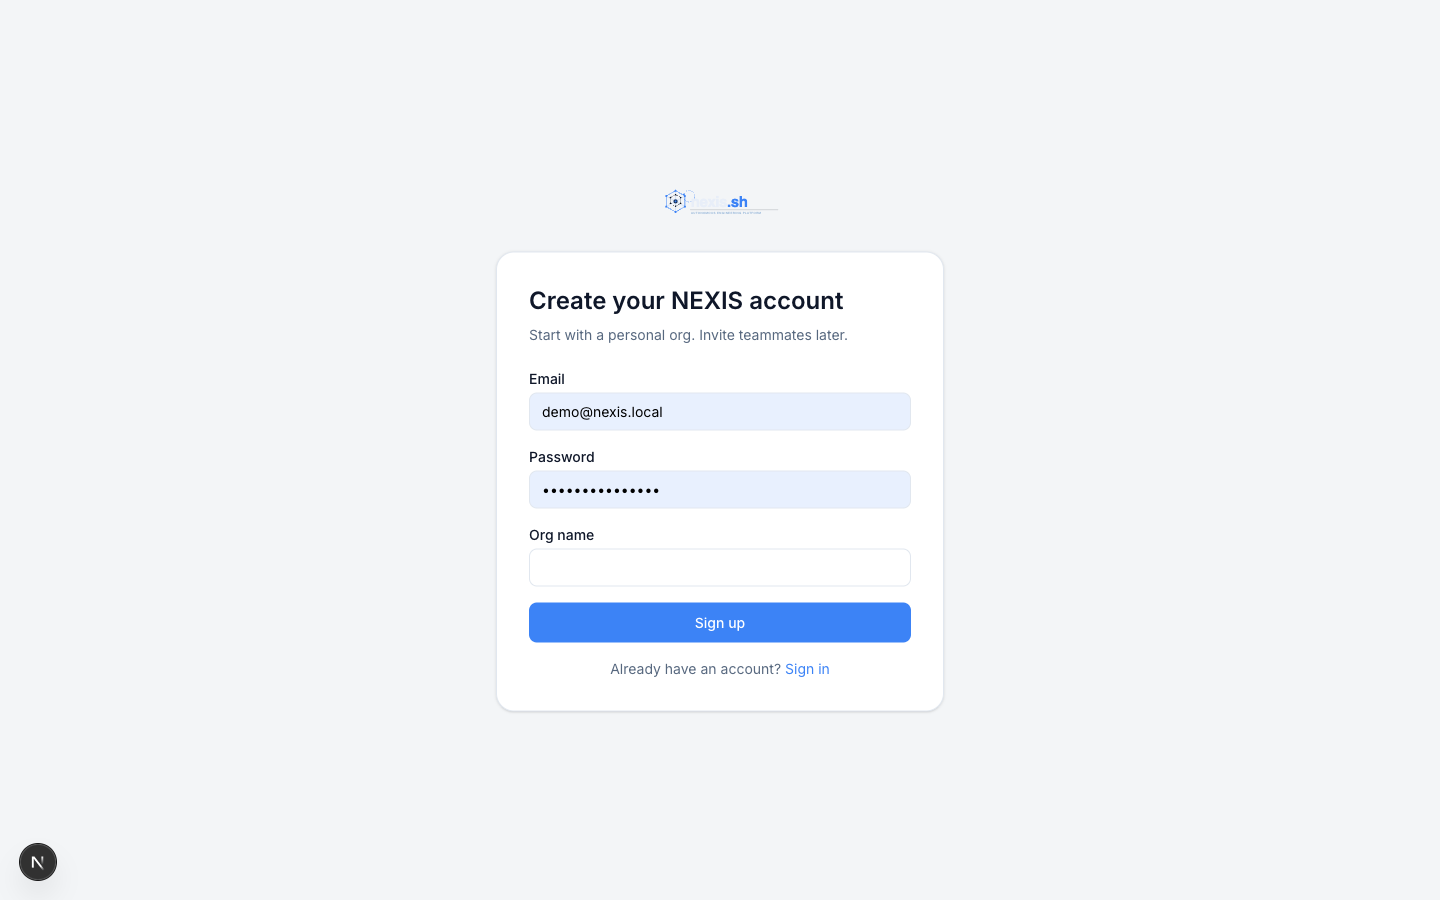
\includegraphics[width=0.85\textwidth]{../assets/screenshots/01-signup.png}
\caption{Sign-Up Screen ( new account registration ).}
\label{fig:signup}
\end{figure}

\begin{figure}[htbp]\centering
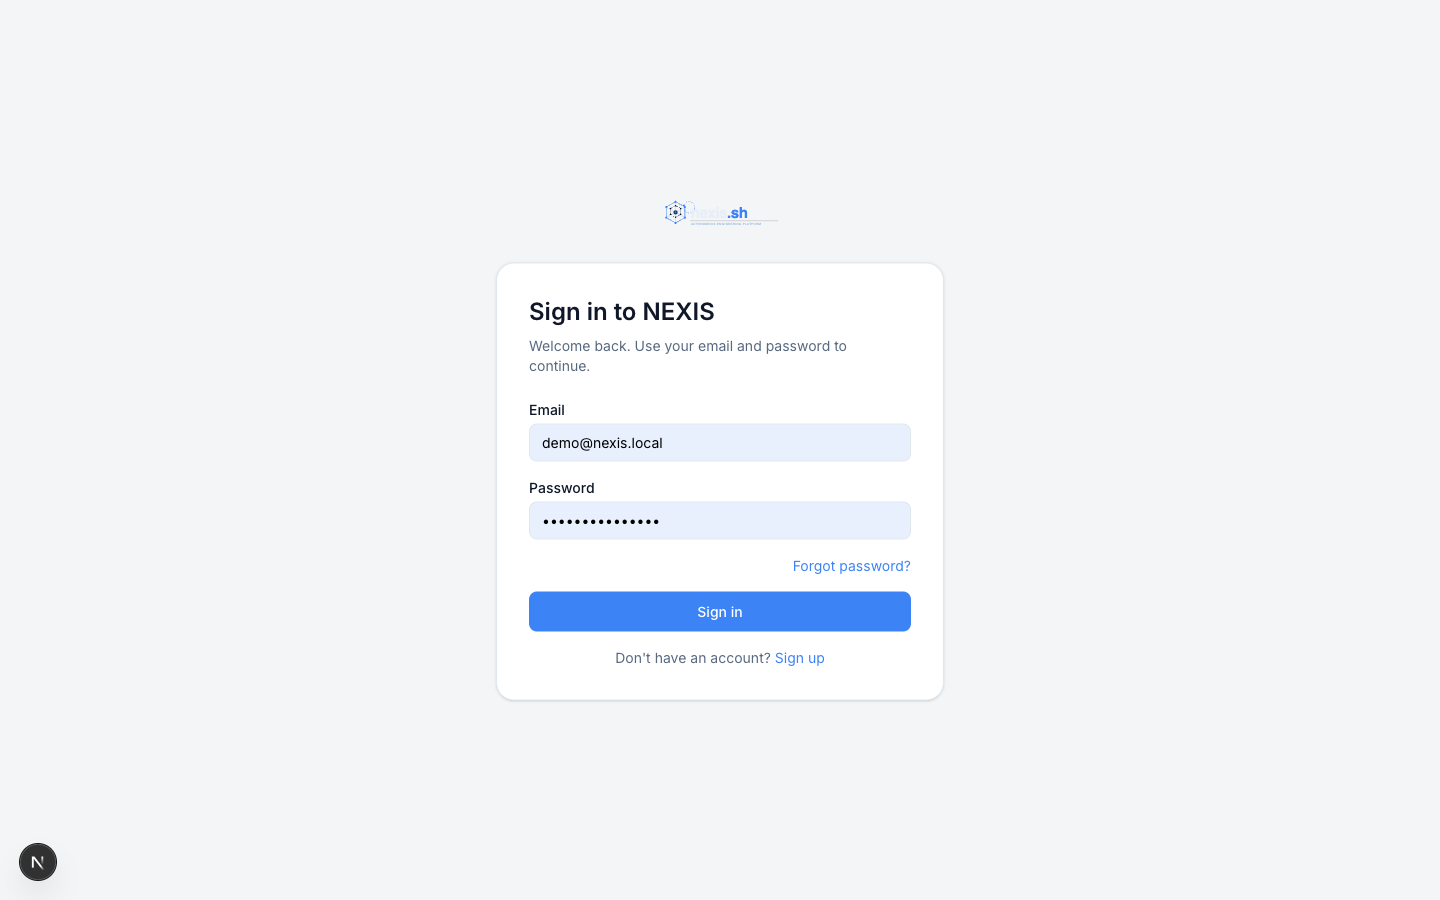
\includegraphics[width=0.85\textwidth]{../assets/screenshots/02-signin.png}
\caption{Sign-In Screen ( JWT session login with HttpOnly cookie ).}
\label{fig:signin}
\end{figure}

\begin{figure}[htbp]\centering
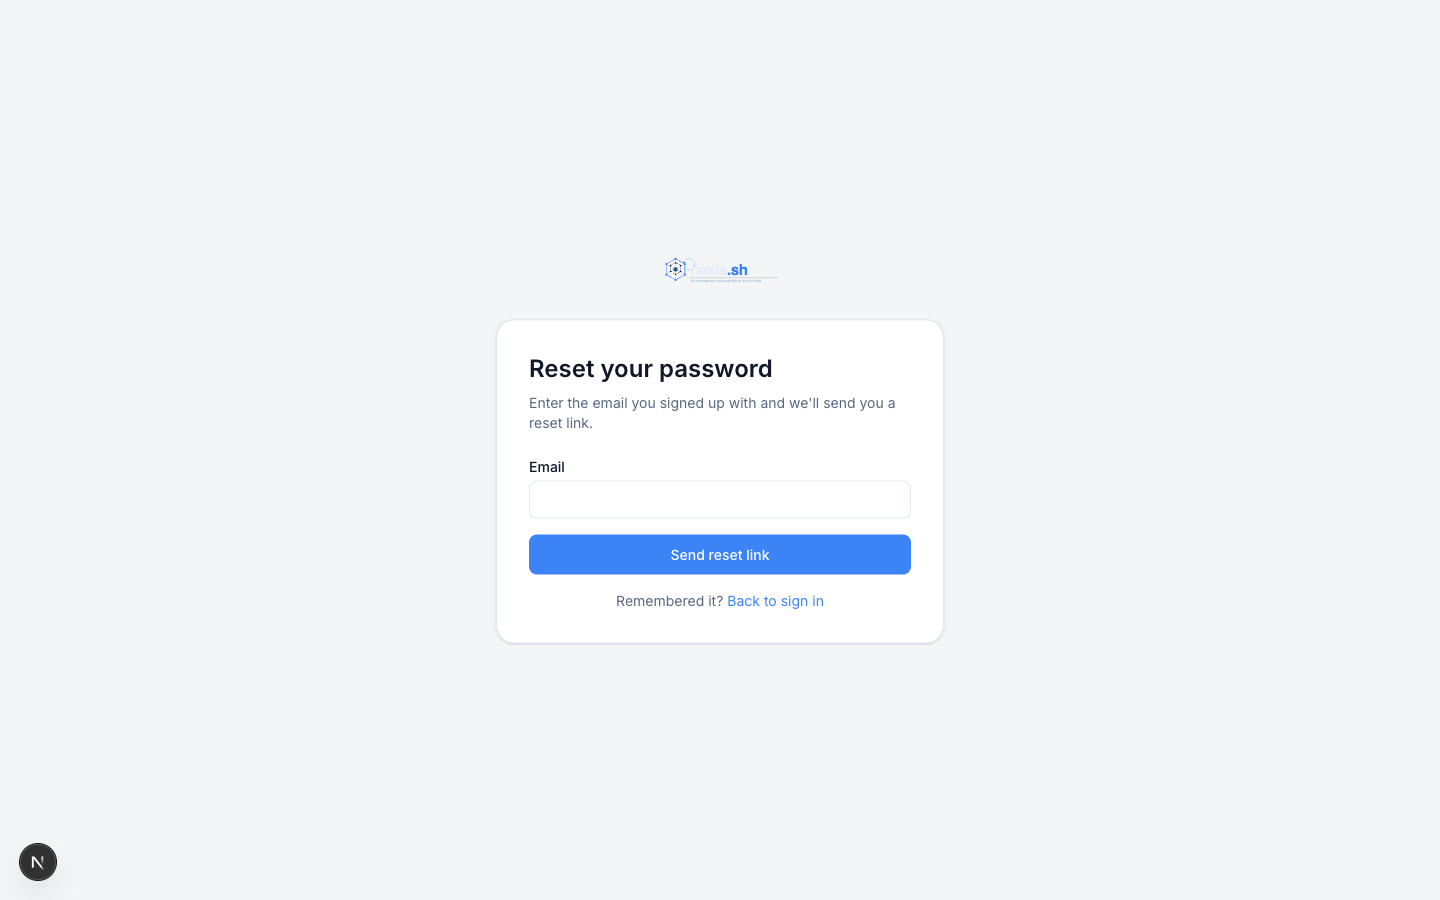
\includegraphics[width=0.85\textwidth]{../assets/screenshots/03-forgot-password.png}
\caption{Forgot-Password Screen ( non-leaky password-reset request ).}
\label{fig:forgot}
\end{figure}

\subsection{Admin / Owner Console}

The console home (Figure~\ref{fig:dashboard}) presents the organisation's
operational state at a glance: KPI tiles for MTTR, recovery success rate,
open incidents and mean tokens per run, an incidents-over-time chart, a
system status panel, a projects health grid, and a recent activity feed.

\begin{figure}[htbp]\centering
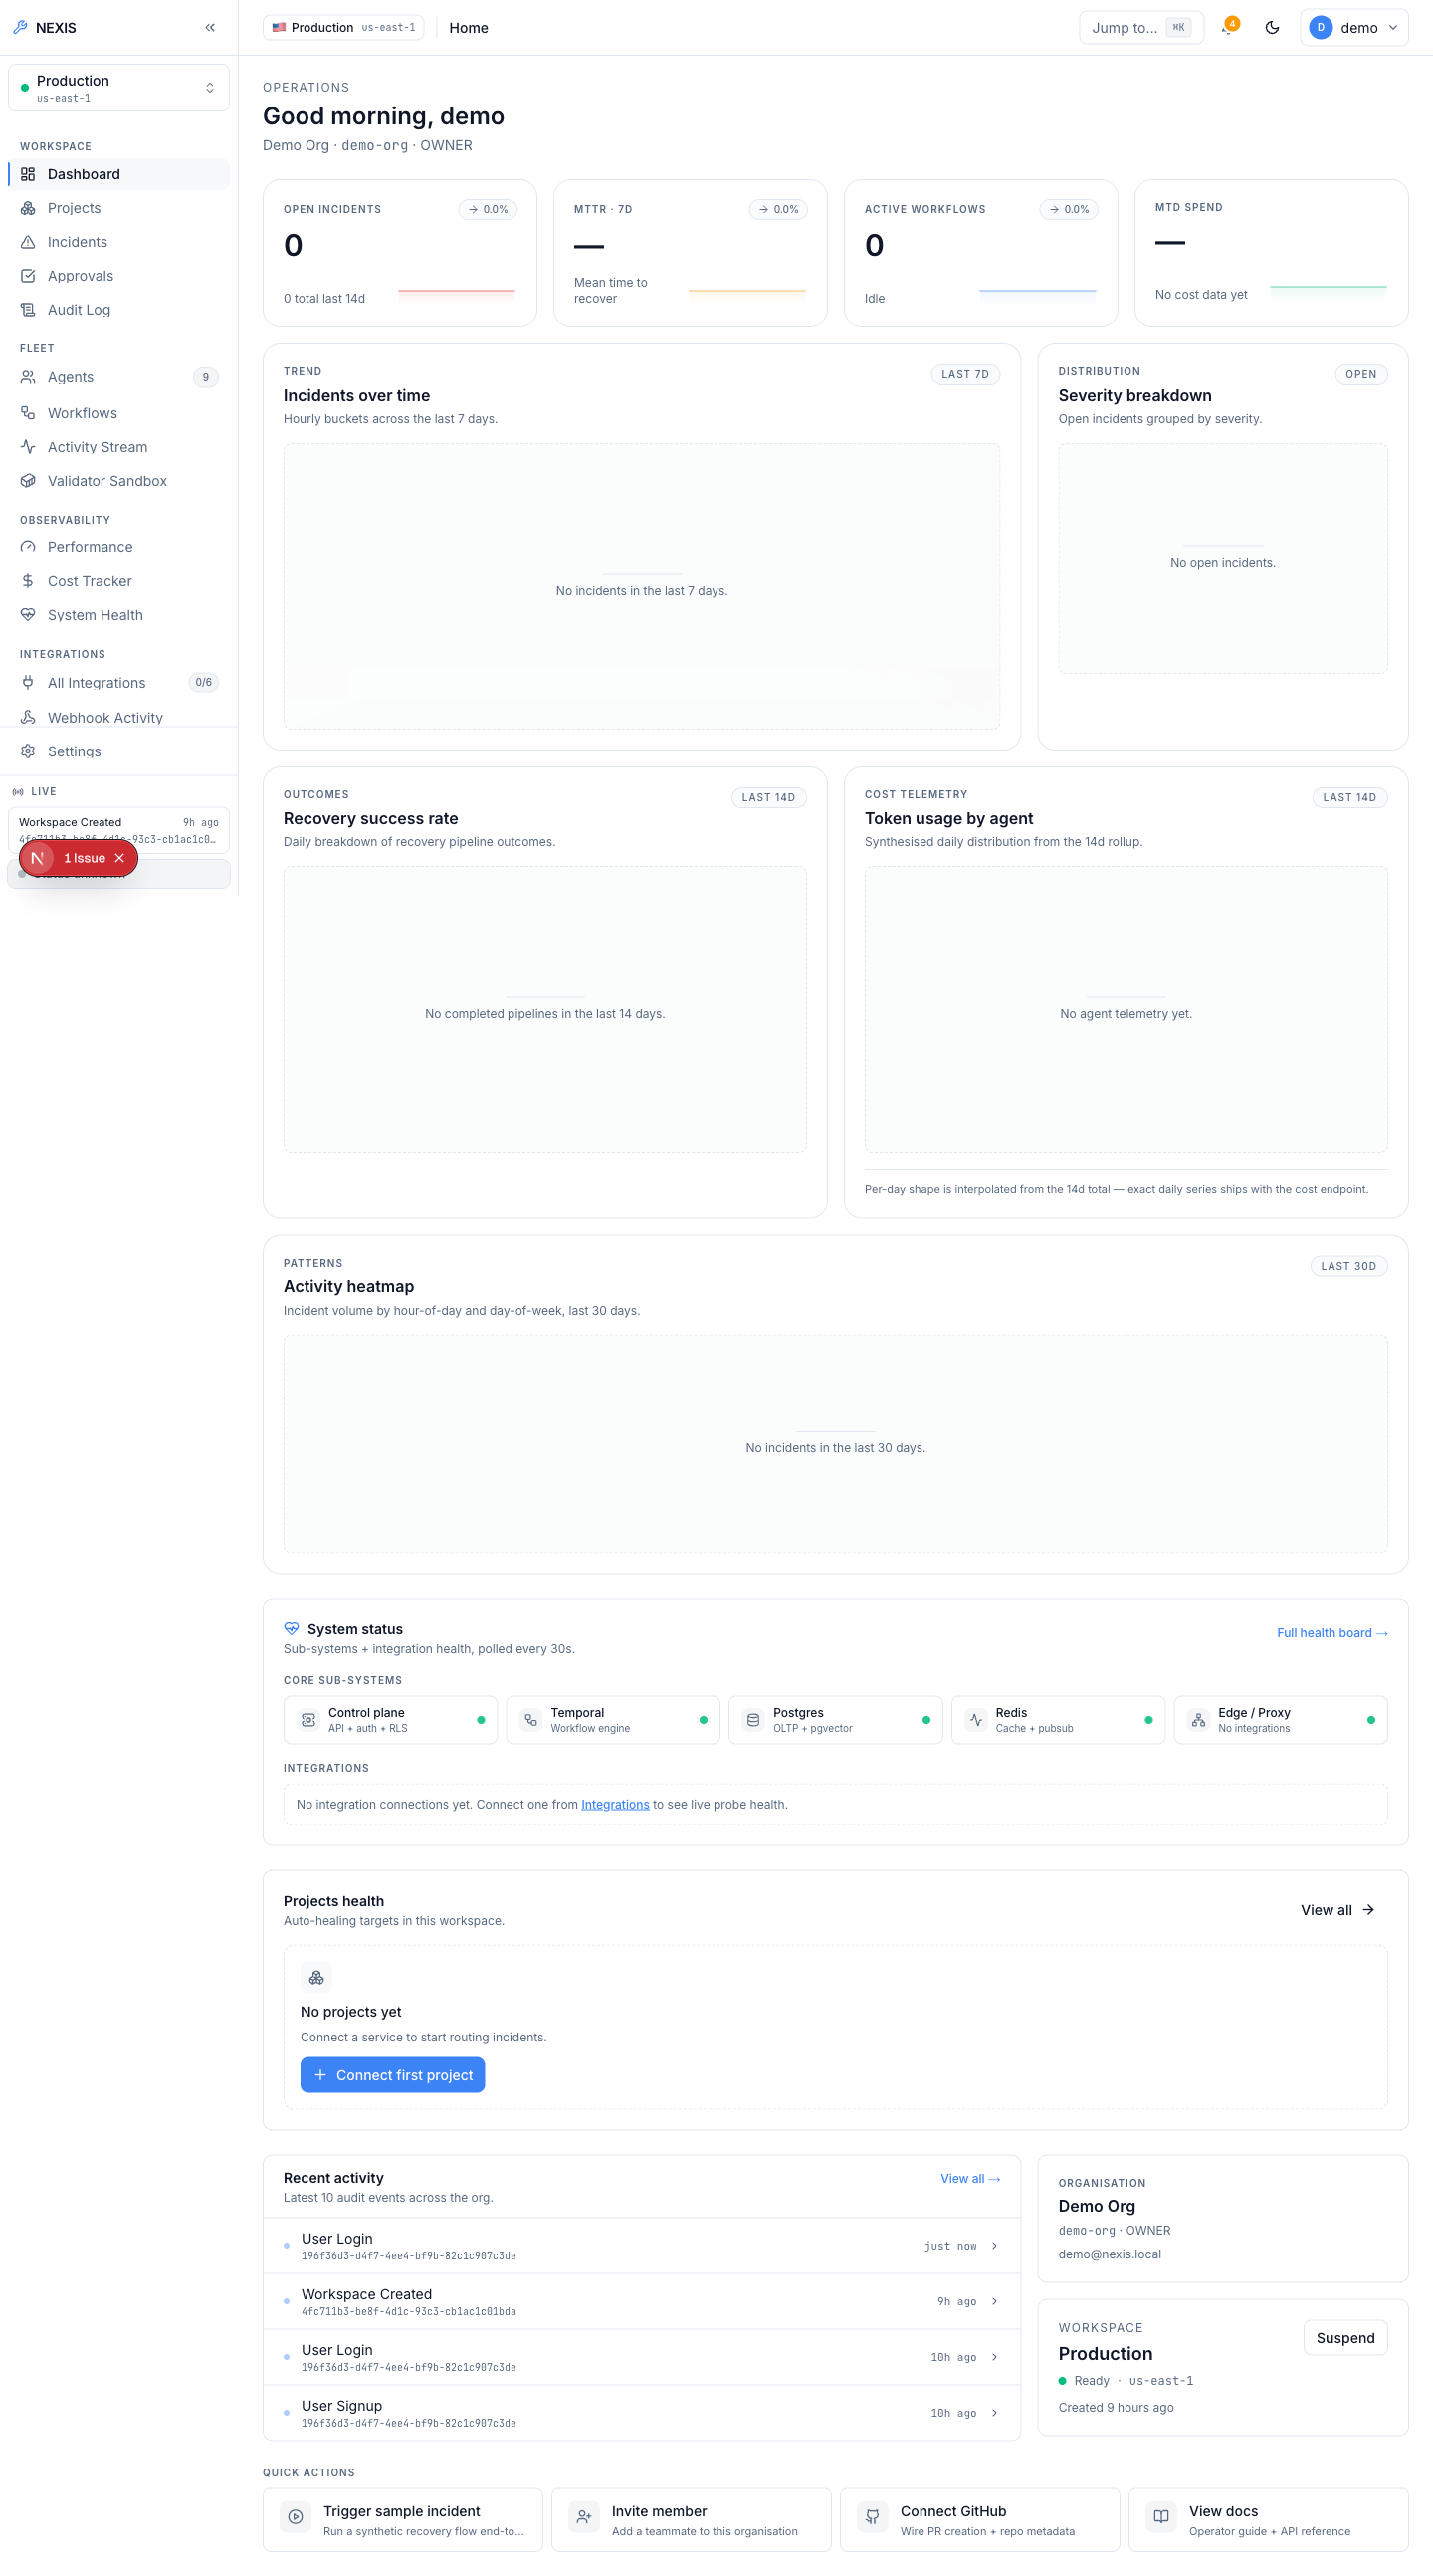
\includegraphics[width=0.85\textwidth]{../assets/screenshots/04-dashboard.png}
\caption{Admin Dashboard ( KPI tiles, incidents-over-time chart, and system status panel ).}
\label{fig:dashboard}
\end{figure}

The Agents page (Figure~\ref{fig:agents}) lists the full nine-agent fleet
across both layers --- the five Execution Team agents (Architect, Backend,
QA, DevOps, Data Engineer) and the Self-Healing Loop agents (Sentinel,
Pathfinder, Synthesiser, Validator) --- with each agent's role and status.

\begin{figure}[htbp]\centering
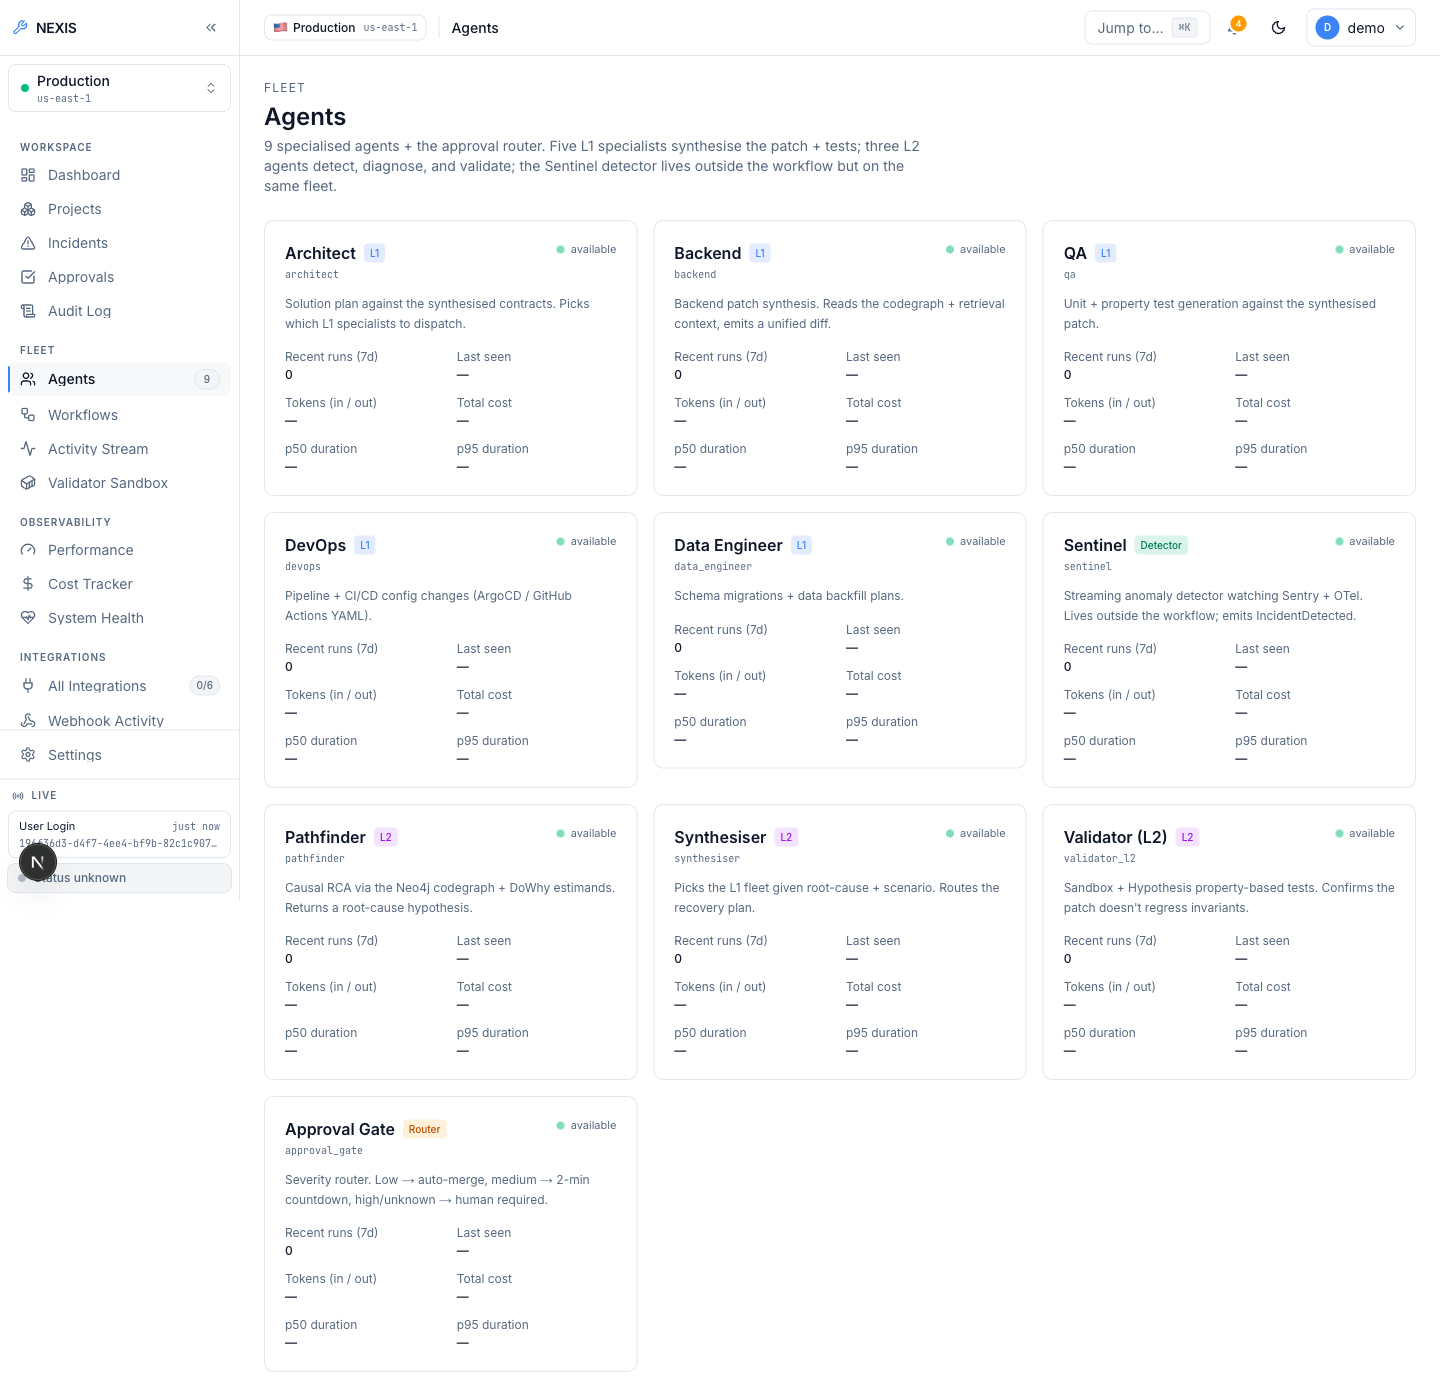
\includegraphics[width=0.85\textwidth]{../assets/screenshots/05-agents.png}
\caption{Agents Screen ( the nine-agent fleet roster across both layers ).}
\label{fig:agents}
\end{figure}

The Workflows page (Figure~\ref{fig:workflows}) lists RecoveryPipeline
executions; the Activity Stream (Figure~\ref{fig:activity}) is the
org-wide live event feed; and the Validator Sandbox console page
(Figure~\ref{fig:sandbox}) surfaces the Docker-sandboxed shadow-execution
service in which every candidate patch is run against its QA-generated
property tests before it may reach the approval gate.

\begin{figure}[htbp]\centering
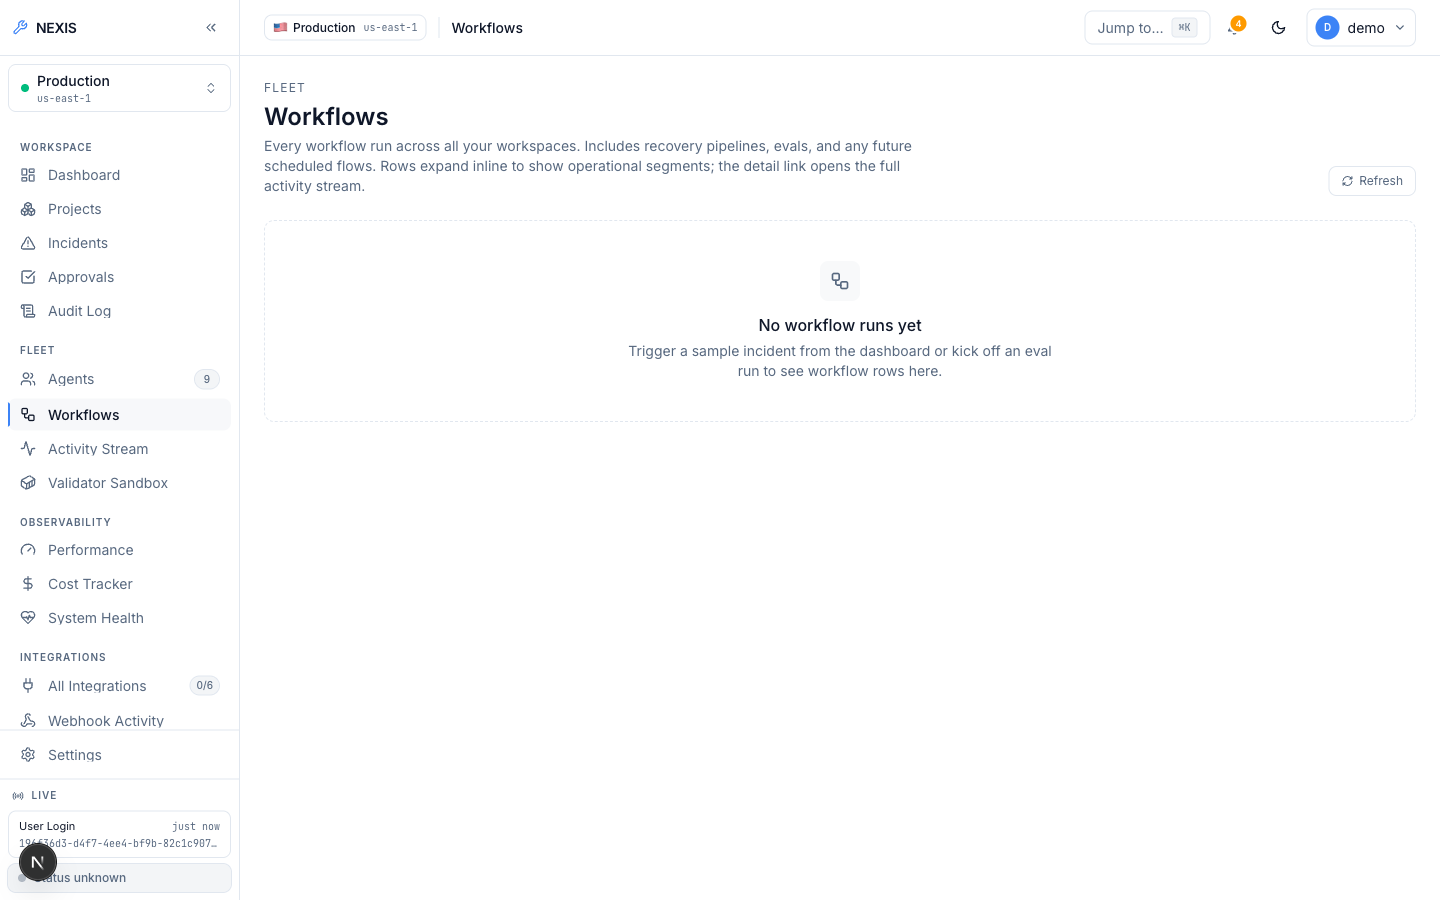
\includegraphics[width=0.85\textwidth]{../assets/screenshots/06-workflows.png}
\caption{Workflows Screen ( RecoveryPipeline run listing ).}
\label{fig:workflows}
\end{figure}

\begin{figure}[htbp]\centering
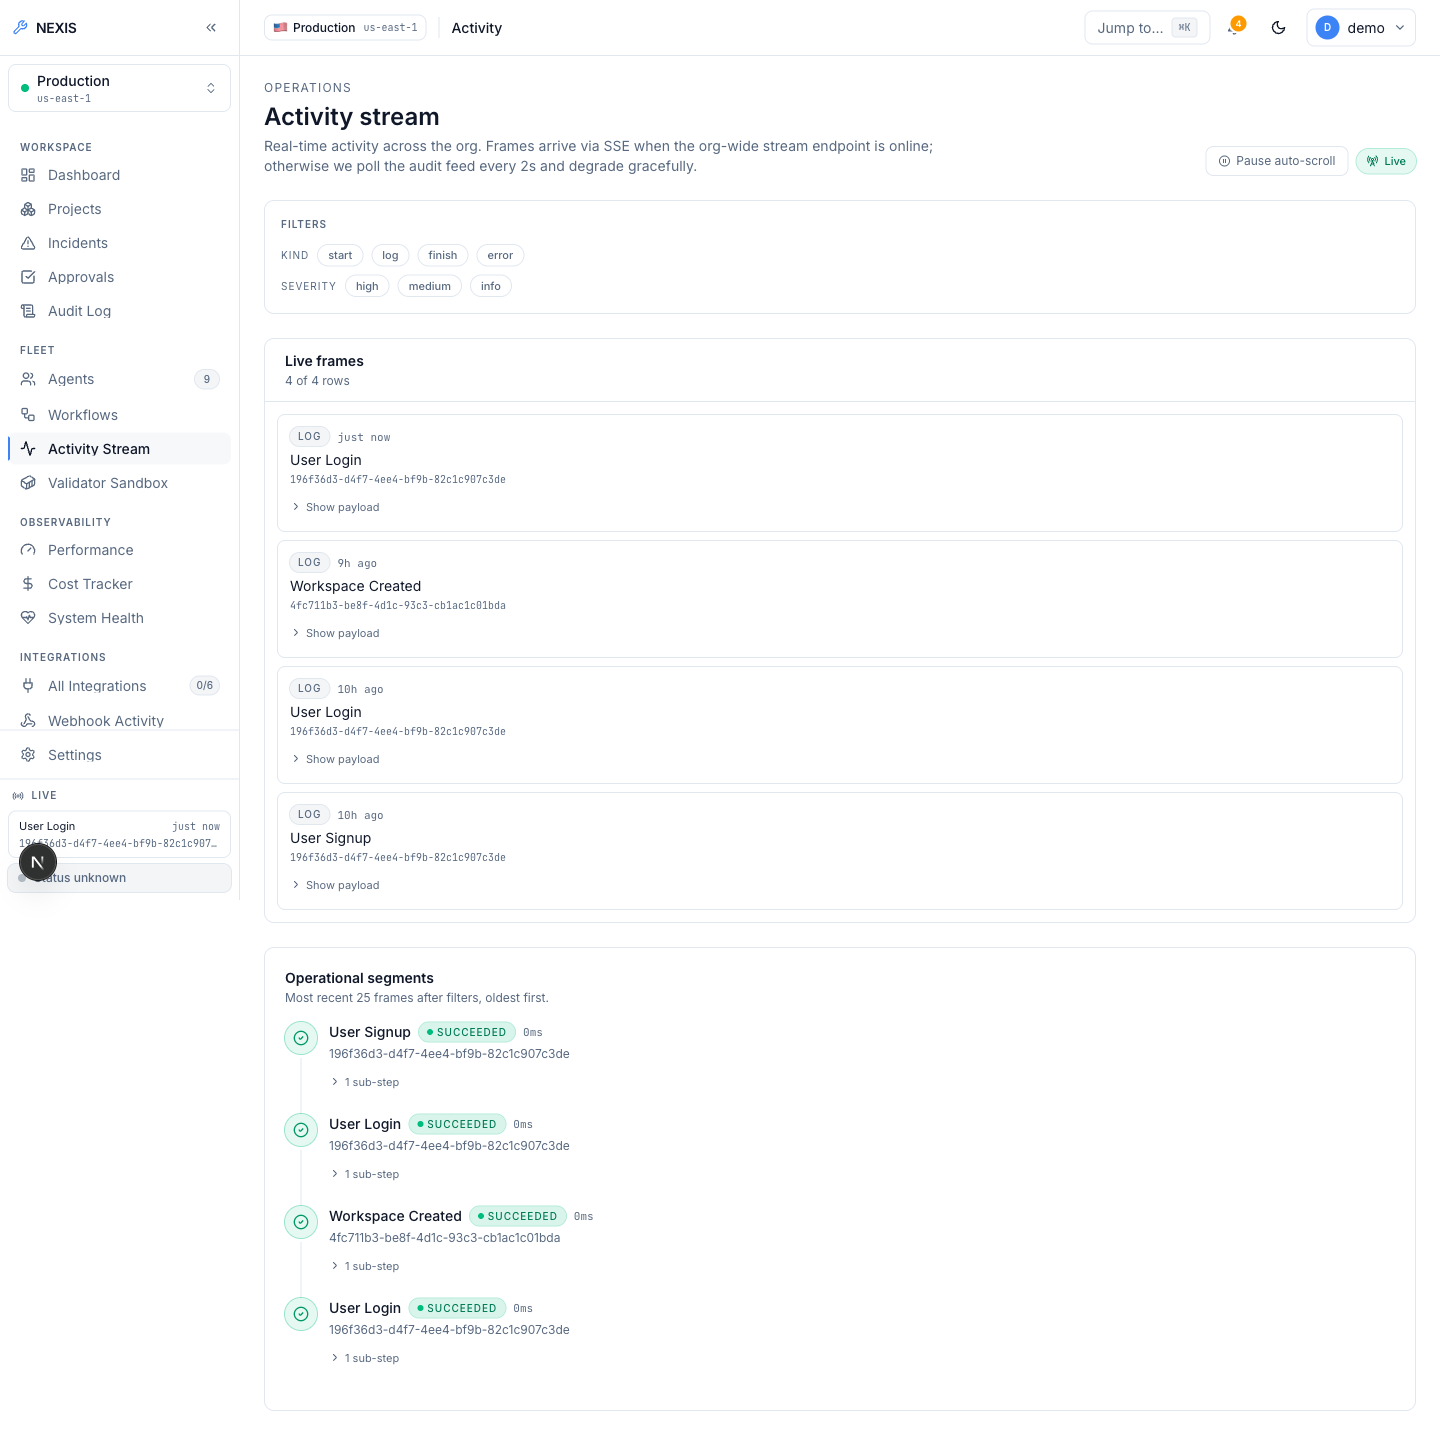
\includegraphics[width=0.85\textwidth]{../assets/screenshots/07-activity-stream.png}
\caption{Activity Stream ( organisation-wide live event feed ).}
\label{fig:activity}
\end{figure}

\begin{figure}[htbp]\centering
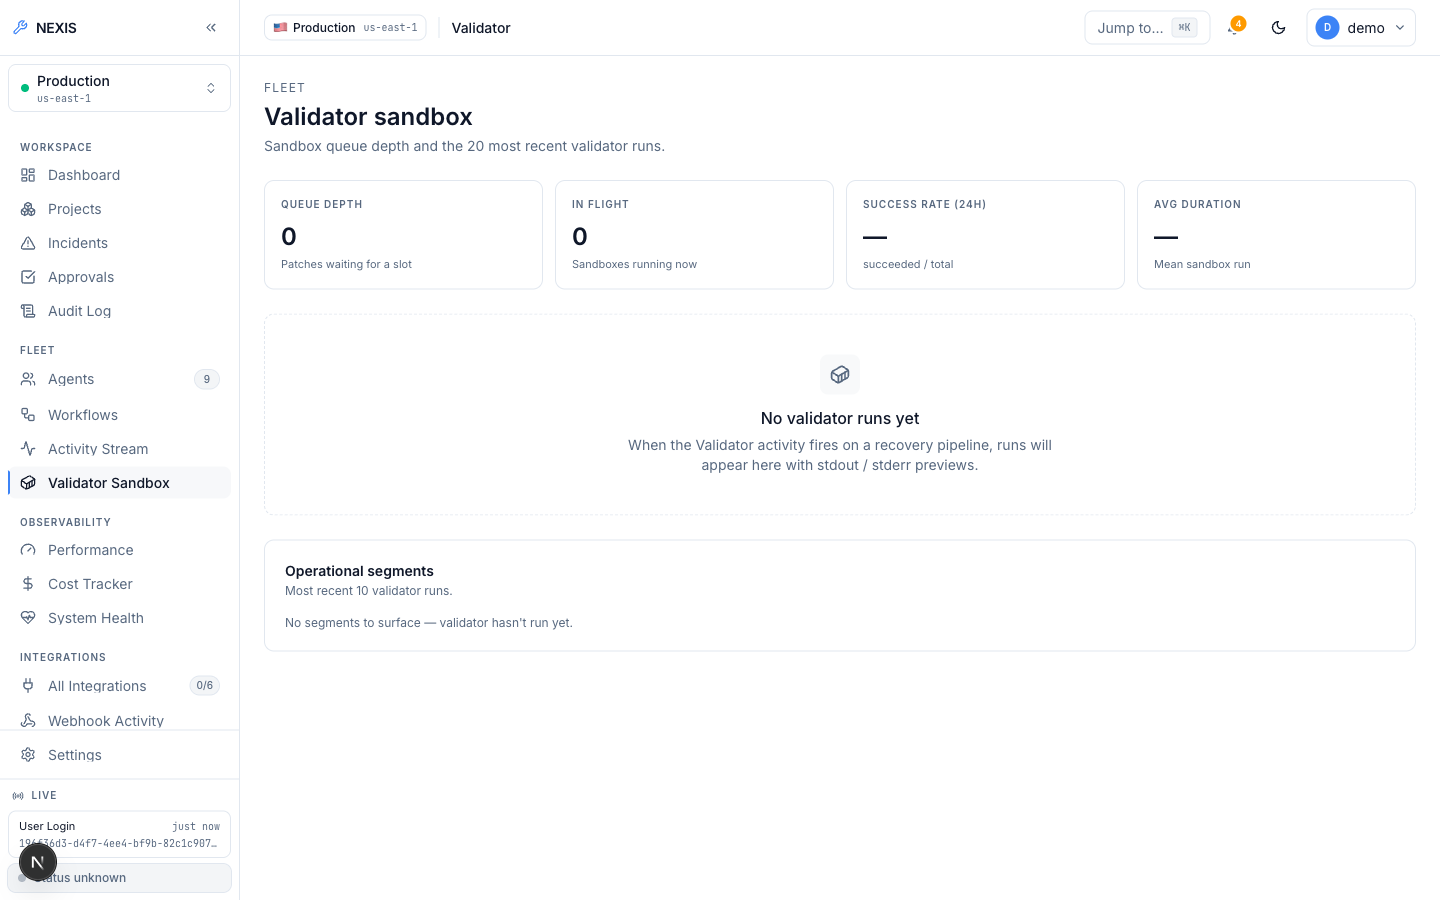
\includegraphics[width=0.85\textwidth]{../assets/screenshots/08-validator-sandbox.png}
\caption{Validator Sandbox Console ( sandboxed shadow execution of candidate patches ).}
\label{fig:sandbox}
\end{figure}

The Audit Log (Figure~\ref{fig:audit}) is append-only and hash-chained: each
entry incorporates the hash of its predecessor, so any tampering with a past
row breaks the chain and is detectable by the cryptographic verify endpoint.
The log supports CSV export for offline review.

\begin{figure}[htbp]\centering
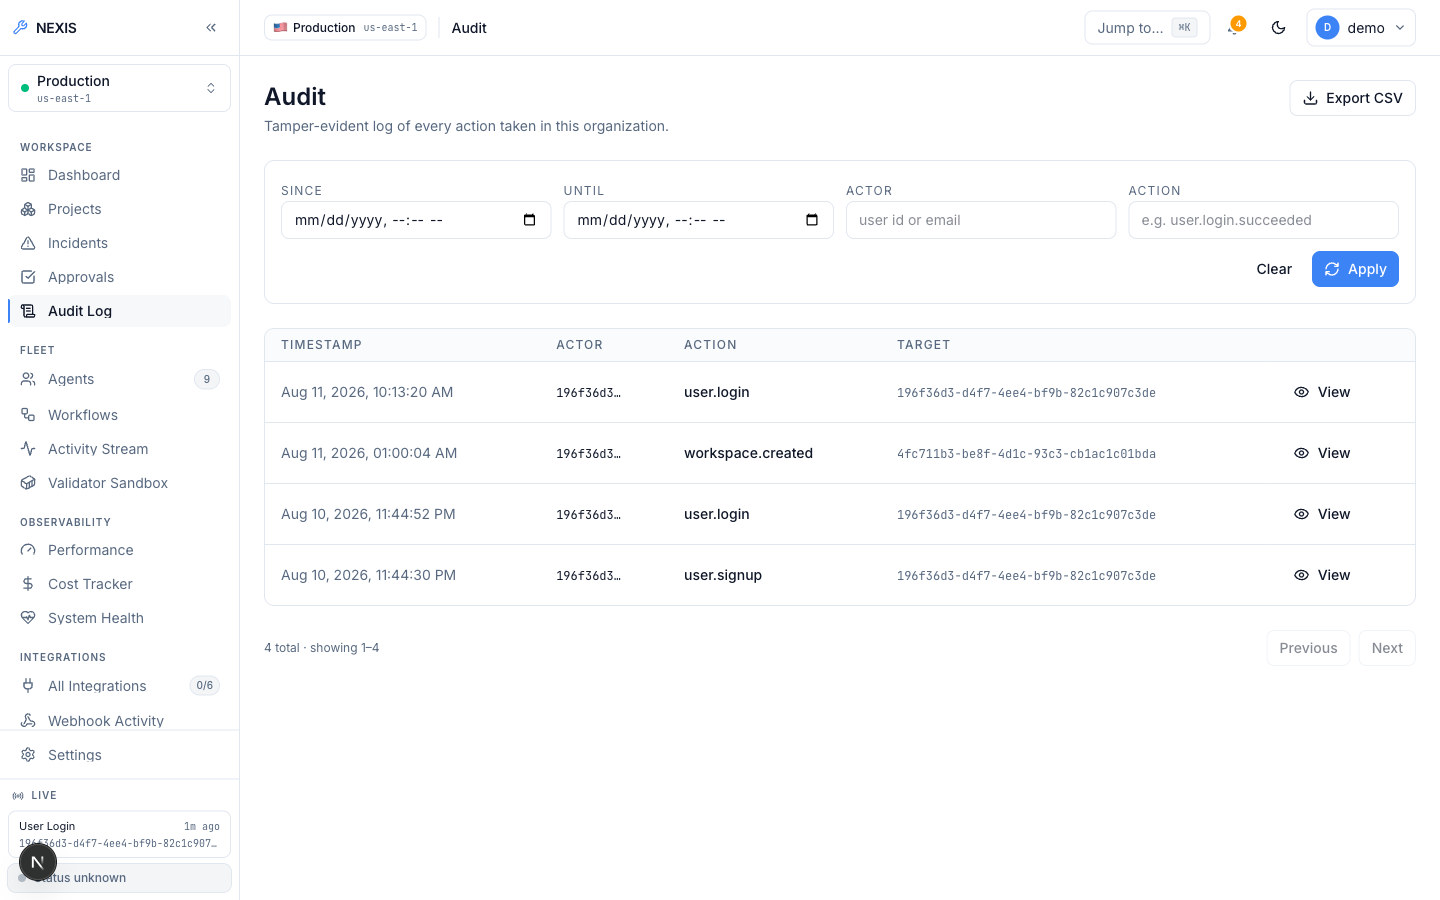
\includegraphics[width=0.85\textwidth]{../assets/screenshots/11-audit-log.png}
\caption{Audit Log ( append-only, hash-chained entries with CSV export ).}
\label{fig:audit}
\end{figure}

\subsection{Members, Roles, and Sessions}

The Members settings page (Figure~\ref{fig:members}) lists the
organisation's members with their roles (owner, admin, member) and exposes
the intelligent role-recommendation panel. This panel is backed by the real
heuristic engine described in Chapter~4, not a mock: it evaluates concrete
signals already captured in the schema --- a member with five or more
admin-gated audit-log actions in 30 days who is not yet an admin, an admin
with no login in 90 or more days, and an active admin with zero admin-gated
actions --- and each recommendation carries a plain-language rationale
naming the specific evidence numbers behind it. An admin can accept the
recommendation (applying the role change under an optimistic-concurrency
guard) or dismiss it, which starts a 30-day per-rule cool-down.

\begin{figure}[htbp]\centering
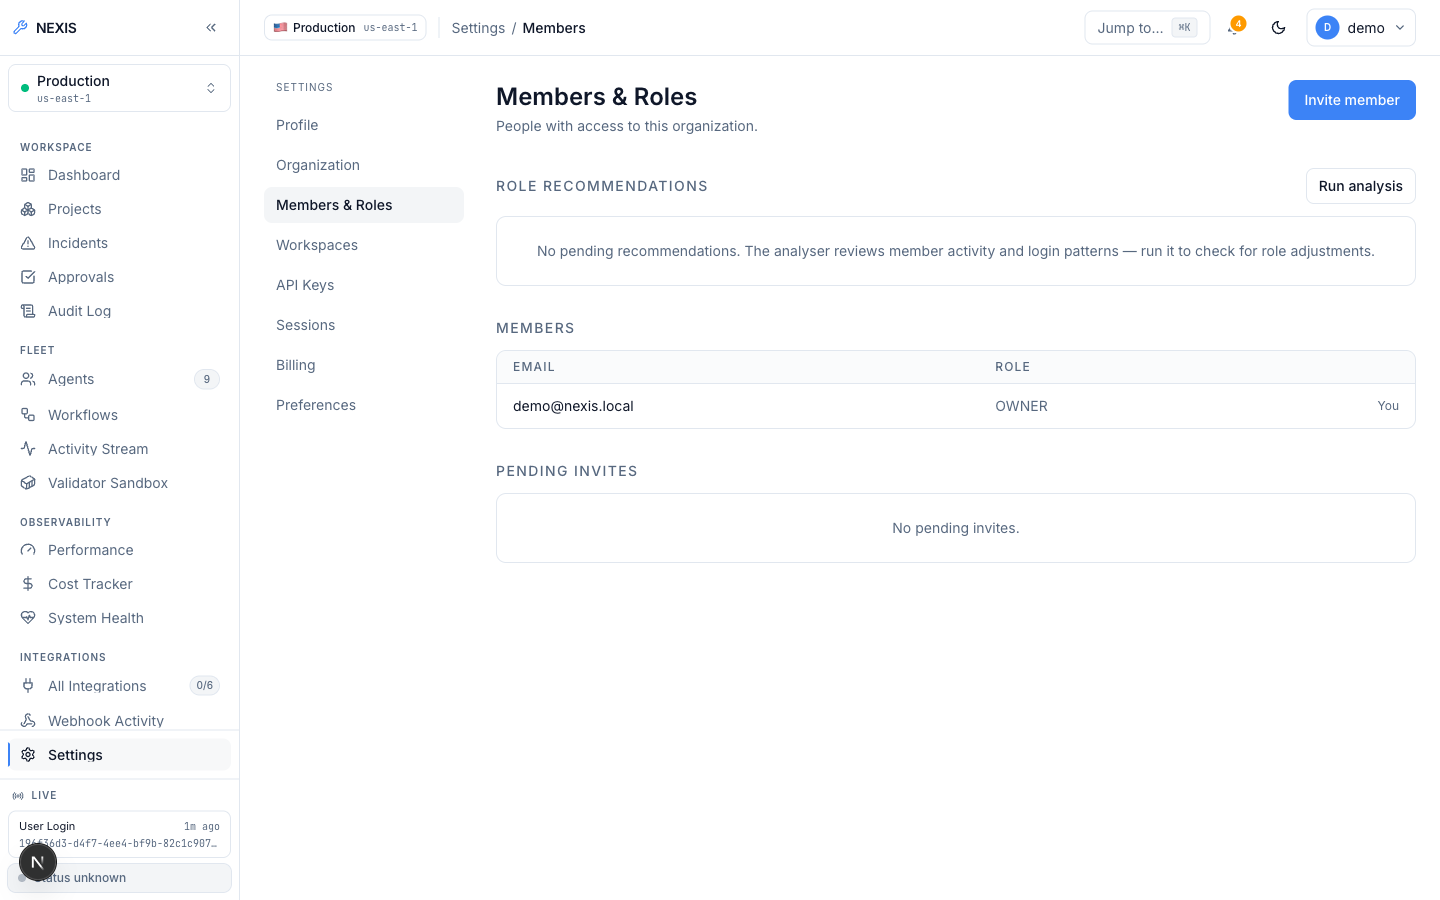
\includegraphics[width=0.85\textwidth]{../assets/screenshots/13-settings-members.png}
\caption{Members Settings ( members list with the heuristic role-recommendation panel ).}
\label{fig:members}
\end{figure}

Session management (Figure~\ref{fig:sessions}) lists every active session
with its device, IP address, user agent, and last-seen time; any session can
be revoked remotely, and the caller's own session is marked with a ``This
device'' badge. API keys (Figure~\ref{fig:apikeys}) are scoped bearer tokens
(\code{nx\_live\_...}) that can be created, listed, and revoked. Billing
(Figure~\ref{fig:billing}) surfaces Stripe~\cite{stripe} usage and payment
method management, and the Organization page (Figure~\ref{fig:orgsettings})
holds organisation-level profile settings.

\begin{figure}[htbp]\centering
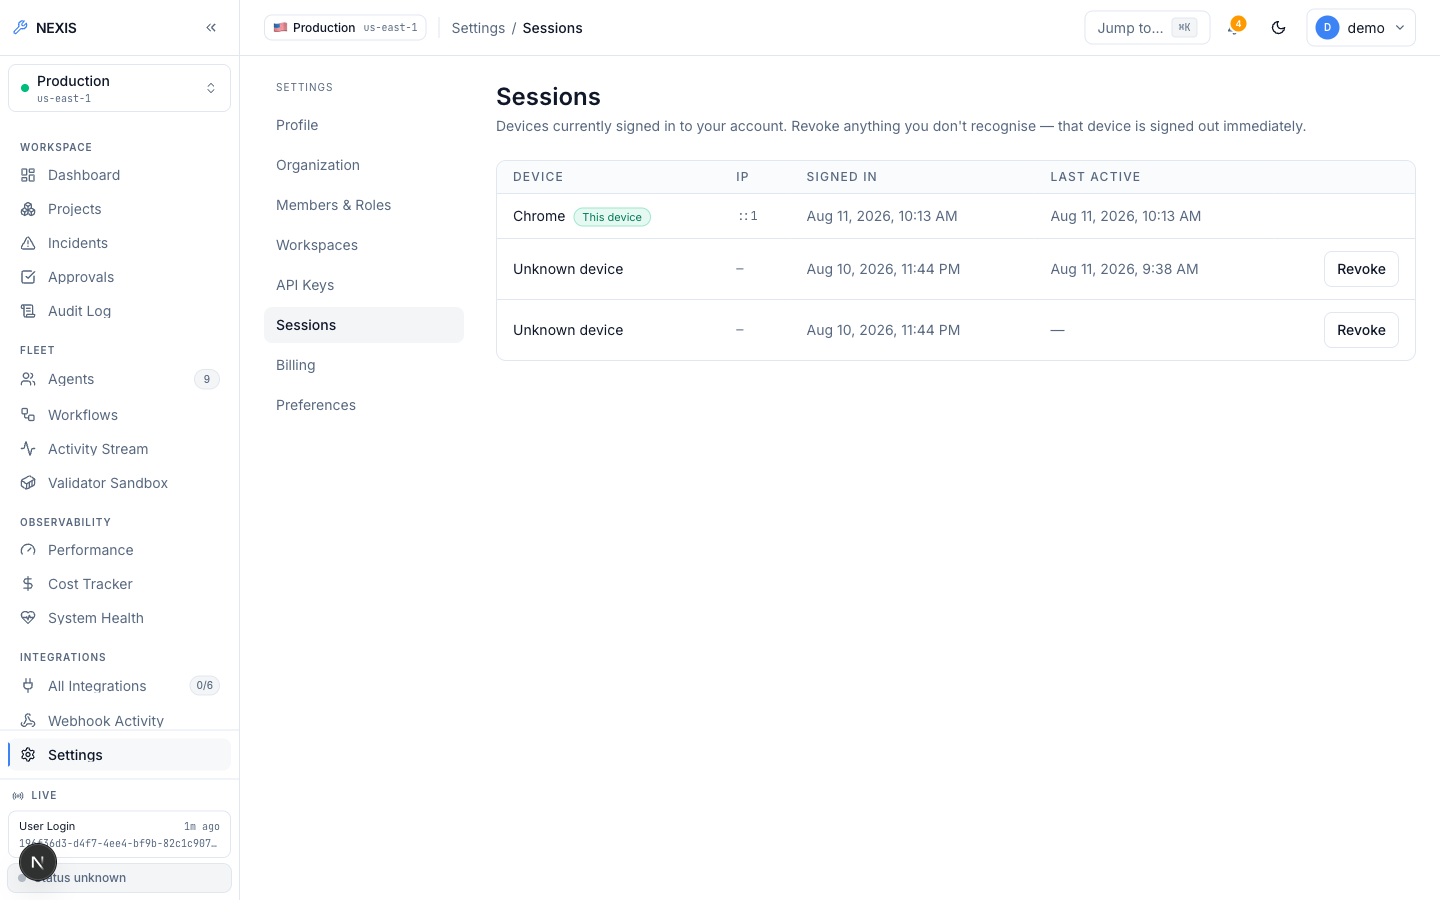
\includegraphics[width=0.85\textwidth]{../assets/screenshots/14-settings-sessions.png}
\caption{Sessions Settings ( active sessions with device, IP, and remote revoke ).}
\label{fig:sessions}
\end{figure}

\begin{figure}[htbp]\centering
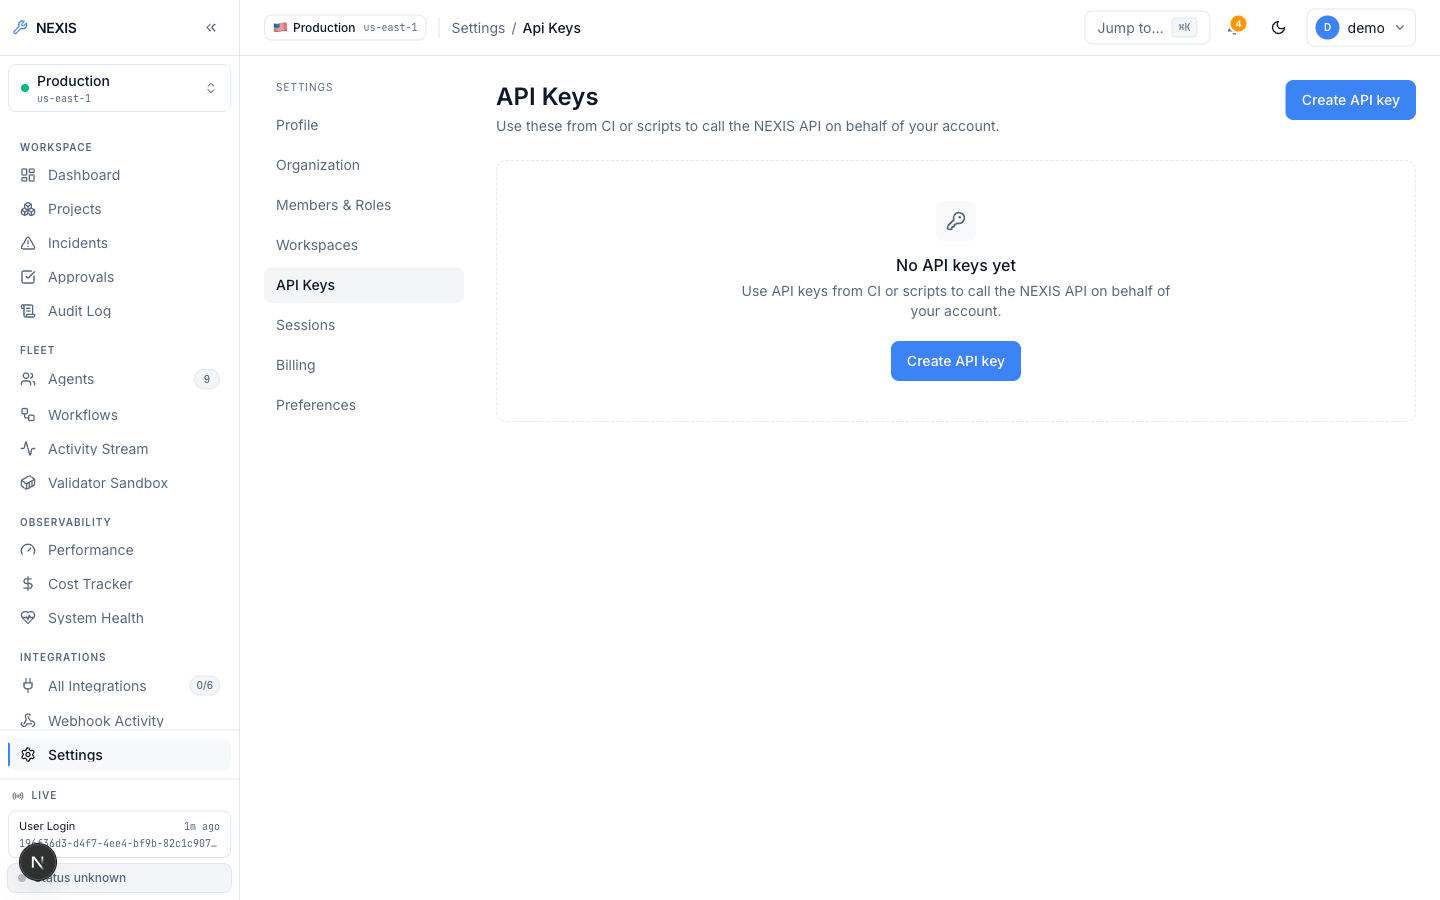
\includegraphics[width=0.85\textwidth]{../assets/screenshots/15-settings-apikeys.png}
\caption{API Keys Settings ( scoped bearer key creation, listing, and revocation ).}
\label{fig:apikeys}
\end{figure}

\begin{figure}[htbp]\centering
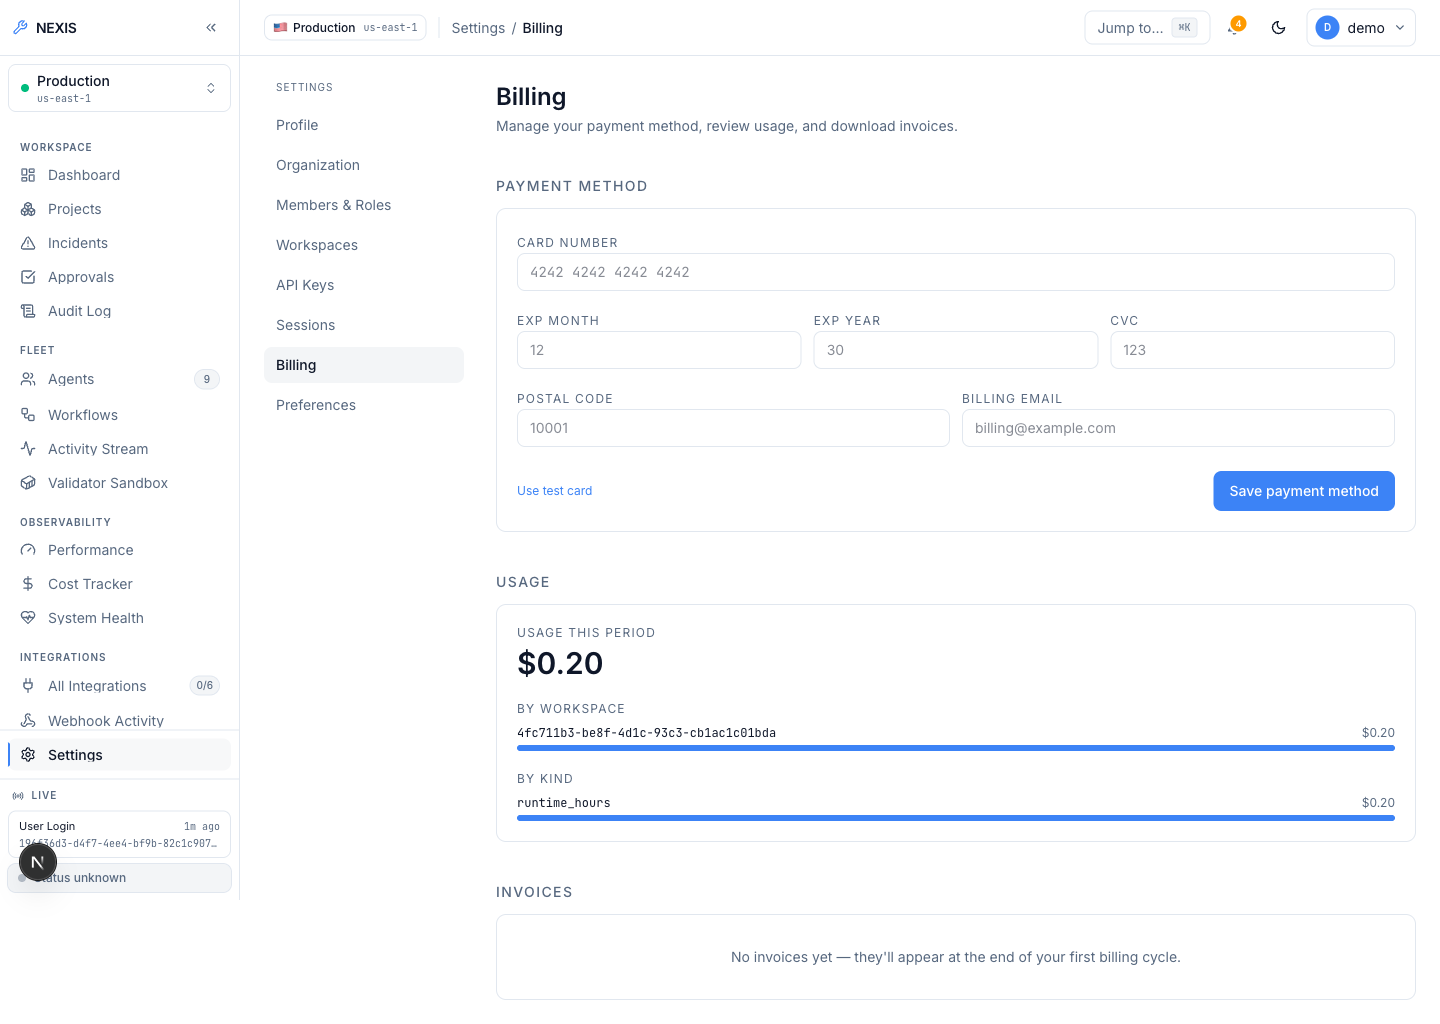
\includegraphics[width=0.85\textwidth]{../assets/screenshots/16-settings-billing.png}
\caption{Billing Settings ( Stripe usage and payment-method management ).}
\label{fig:billing}
\end{figure}

\begin{figure}[htbp]\centering
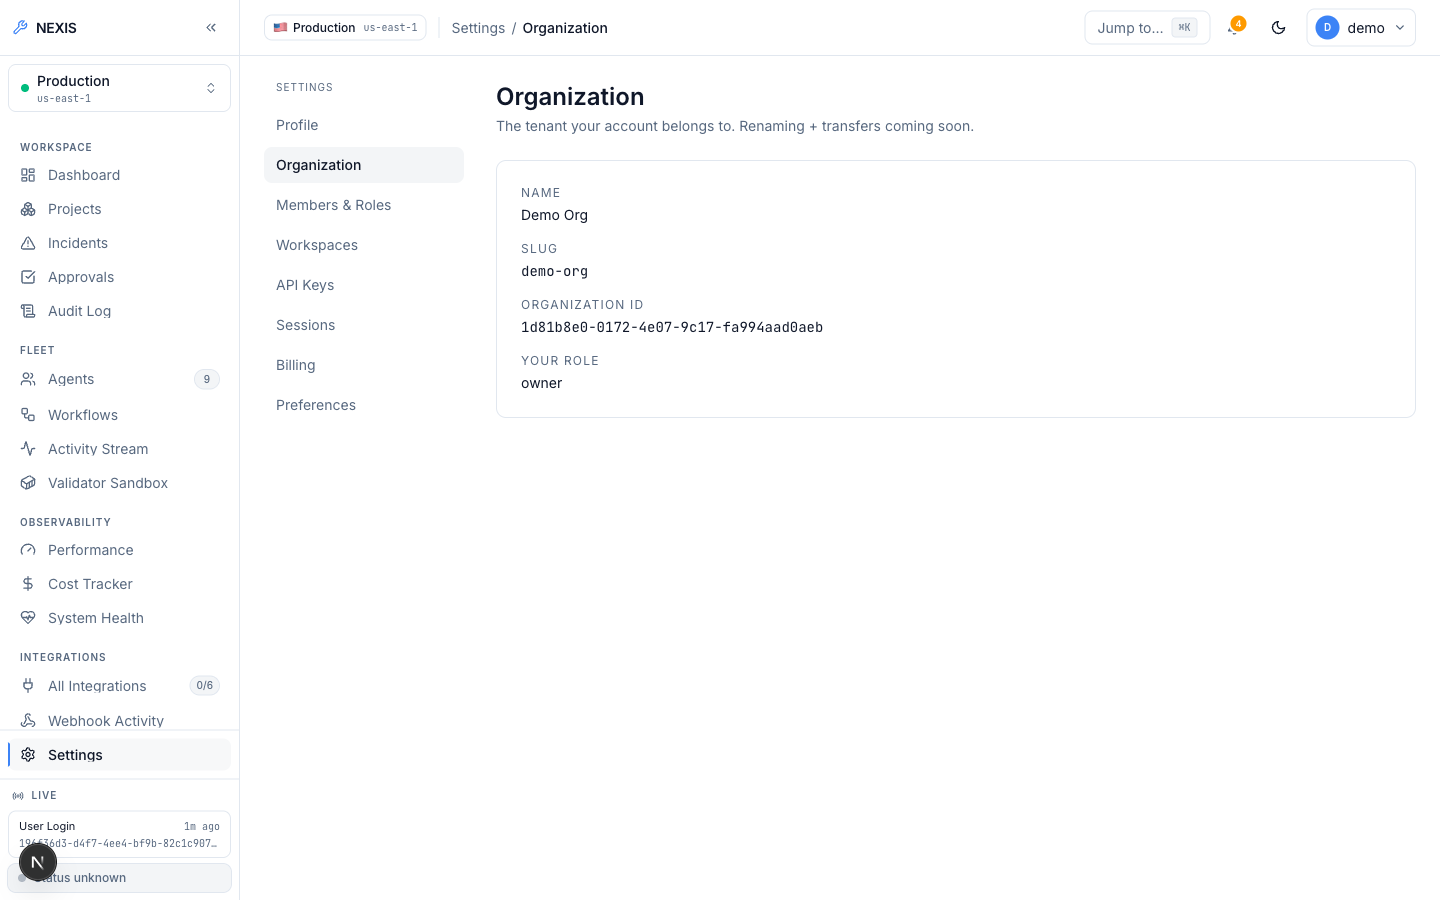
\includegraphics[width=0.85\textwidth]{../assets/screenshots/17-settings-organization.png}
\caption{Organization Settings ( organisation profile management ).}
\label{fig:orgsettings}
\end{figure}

\subsection{Self-Healing Loop --- Live Evidence}
\label{sec:liveevidence}

This subsection is the evidentiary core of the report. It documents two real,
complete, end-to-end executions of the nine-agent RecoveryPipeline against a
live local LLM (Ollama, \code{qwen2.5-coder:14b} and \code{gpt-oss:20b}) ---
one run that timed out at the human approval gate and was safely
auto-rejected, and one run that was approved within the window and succeeded
fully. Both outcomes are shown exactly as they occurred.

The entry point is the Live Demo console (Figure~\ref{fig:livedemo}), which
presents 27 curated fault-scenario cards drawn from a broader fixture
taxonomy spanning application, database, deploy, observability, and security
categories. To be precise about the current state: exactly one of the 27
scenarios is fully wired end-to-end today; the remaining cards are
UI-complete but backend-pending and are labelled ``Coming soon'' in the
interface. The runs documented below were triggered through the wired path.

\begin{figure}[htbp]\centering
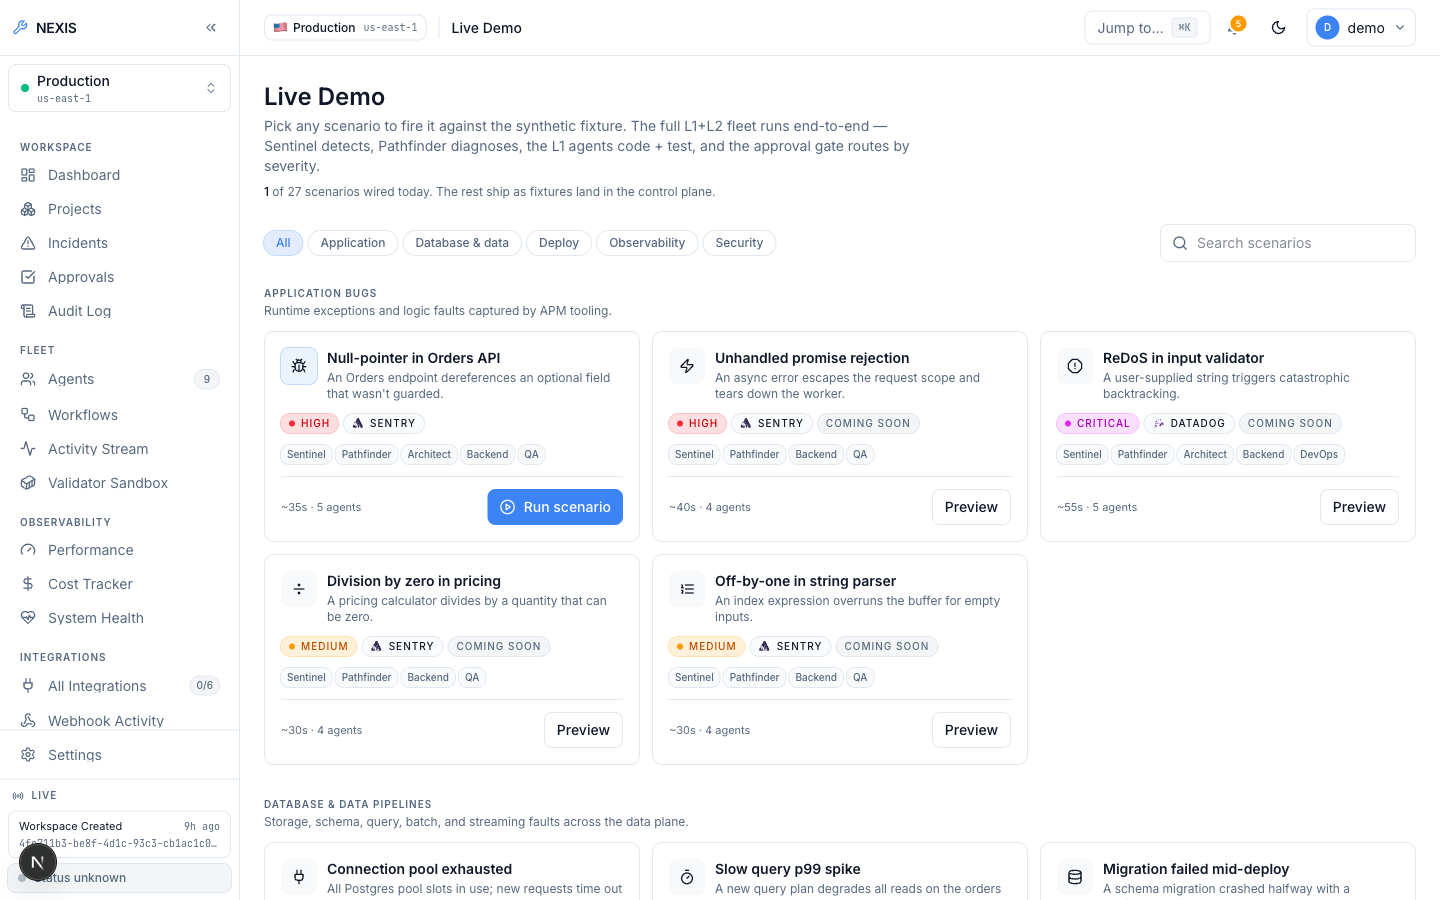
\includegraphics[width=0.85\textwidth]{../assets/screenshots/26-live-demo.png}
\caption{Live Demo Console ( 27-scenario fault-injection picker; one scenario fully wired, the rest backend-pending ).}
\label{fig:livedemo}
\end{figure}

Figure~\ref{fig:livemid} captures the first run genuinely mid-flight. The
Architect, Backend, and QA steps have already completed --- each showing a
real, non-zero token count and cost figure accumulated from actual LLM
calls --- while the DevOps and Data Engineer steps are executing in
parallel. These visible token and cost figures are themselves evidence: a
stubbed or templated pipeline would report zero tokens, whereas every
completed step here carries the token consumption of the model call that
produced its output.

\begin{figure}[htbp]\centering
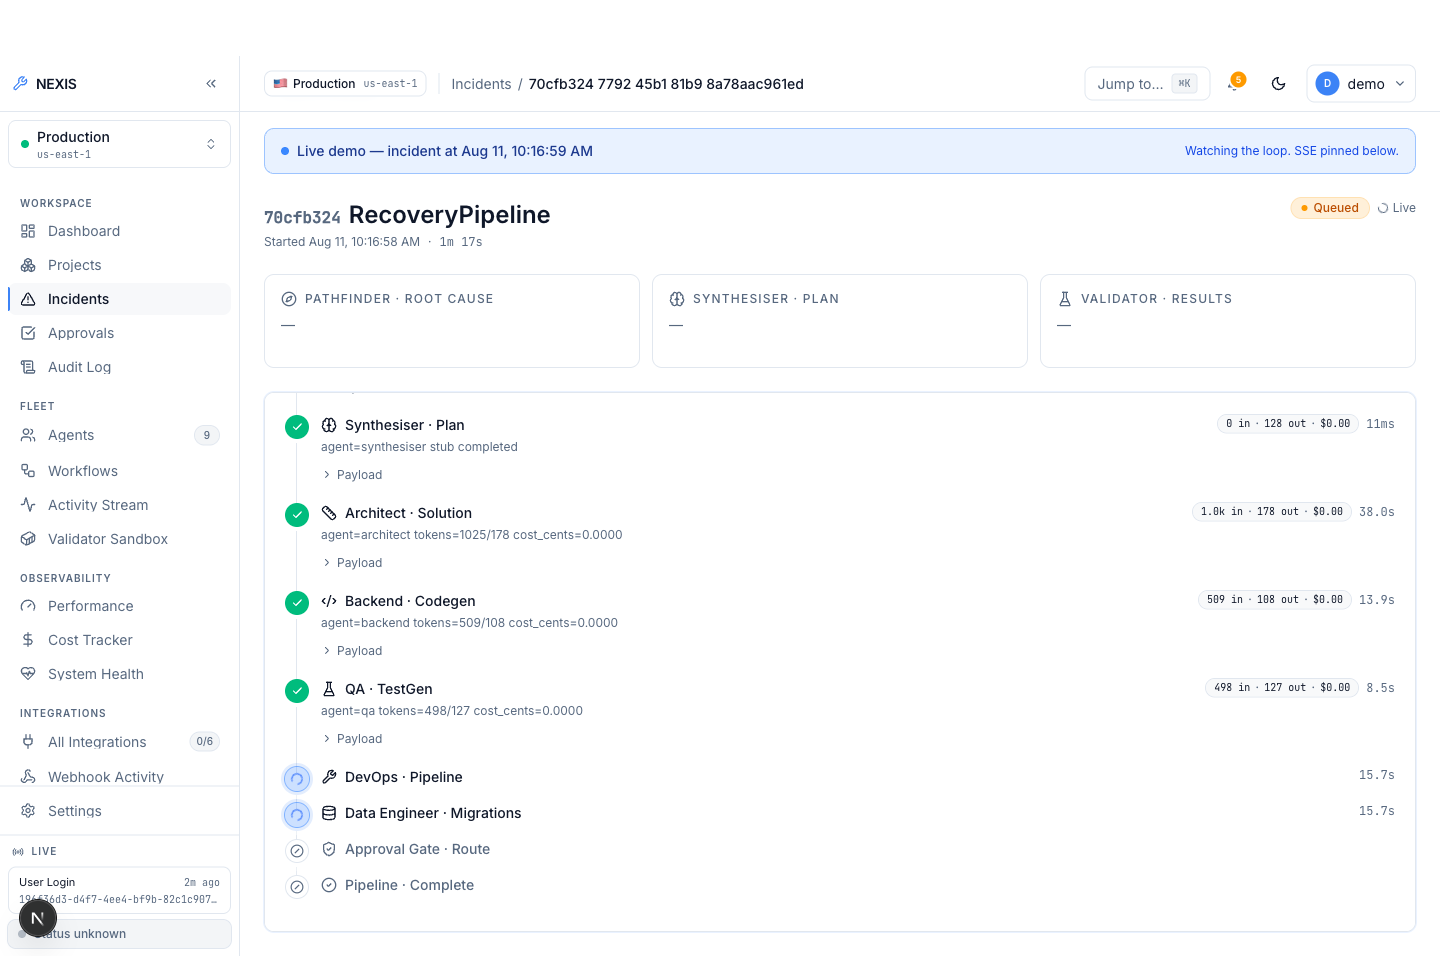
\includegraphics[width=0.85\textwidth]{../assets/screenshots/35-incident-live-progress.png}
\caption{Incident Detail, Mid-Flight ( live pipeline with completed Architect/Backend/QA steps showing real token counts; DevOps and Data Engineer running in parallel ).}
\label{fig:livemid}
\end{figure}

Figure~\ref{fig:livefinal} shows the same run moments later: every Layer-1
and Layer-2 step has completed green --- the patch has been generated,
property-tested, and validated in the sandbox --- and the run now sits at
severity ``Medium'' with approval status ``Pending'', awaiting a human
decision inside the 120-second window.

\begin{figure}[htbp]\centering
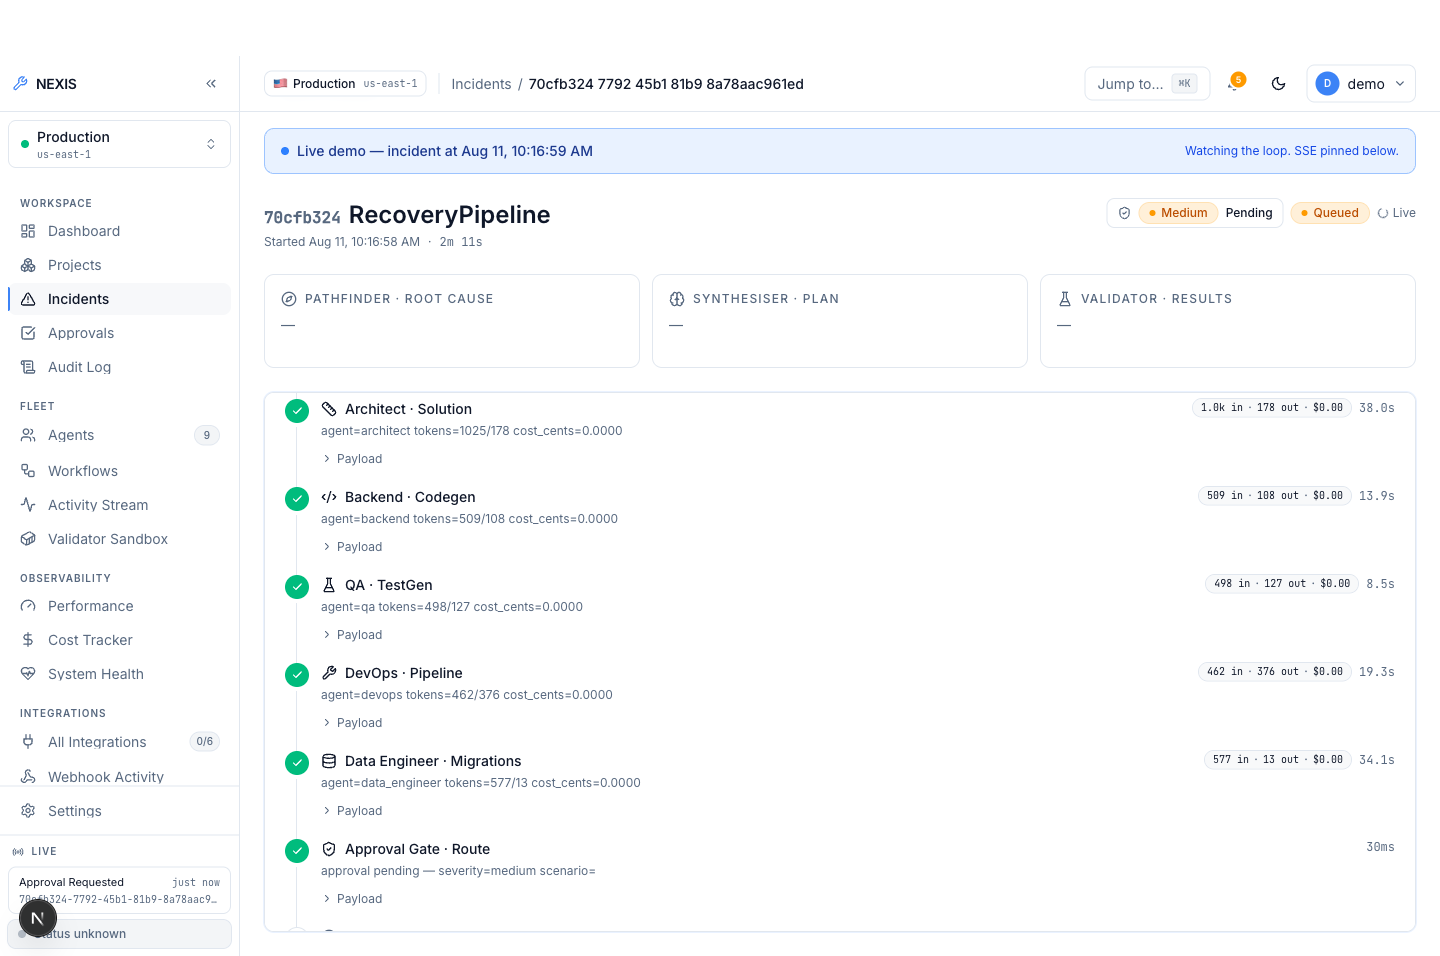
\includegraphics[width=0.85\textwidth]{../assets/screenshots/36-incident-live-final.png}
\caption{Incident Detail, Pipeline Complete ( all L1/L2 steps green; severity Medium, approval Pending ).}
\label{fig:livefinal}
\end{figure}

That pending state is reflected in the Approvals queue
(Figure~\ref{fig:approvals}): a real pending-approval row with the three
human decision actions --- Reject, Modify, and Approve.

\begin{figure}[htbp]\centering
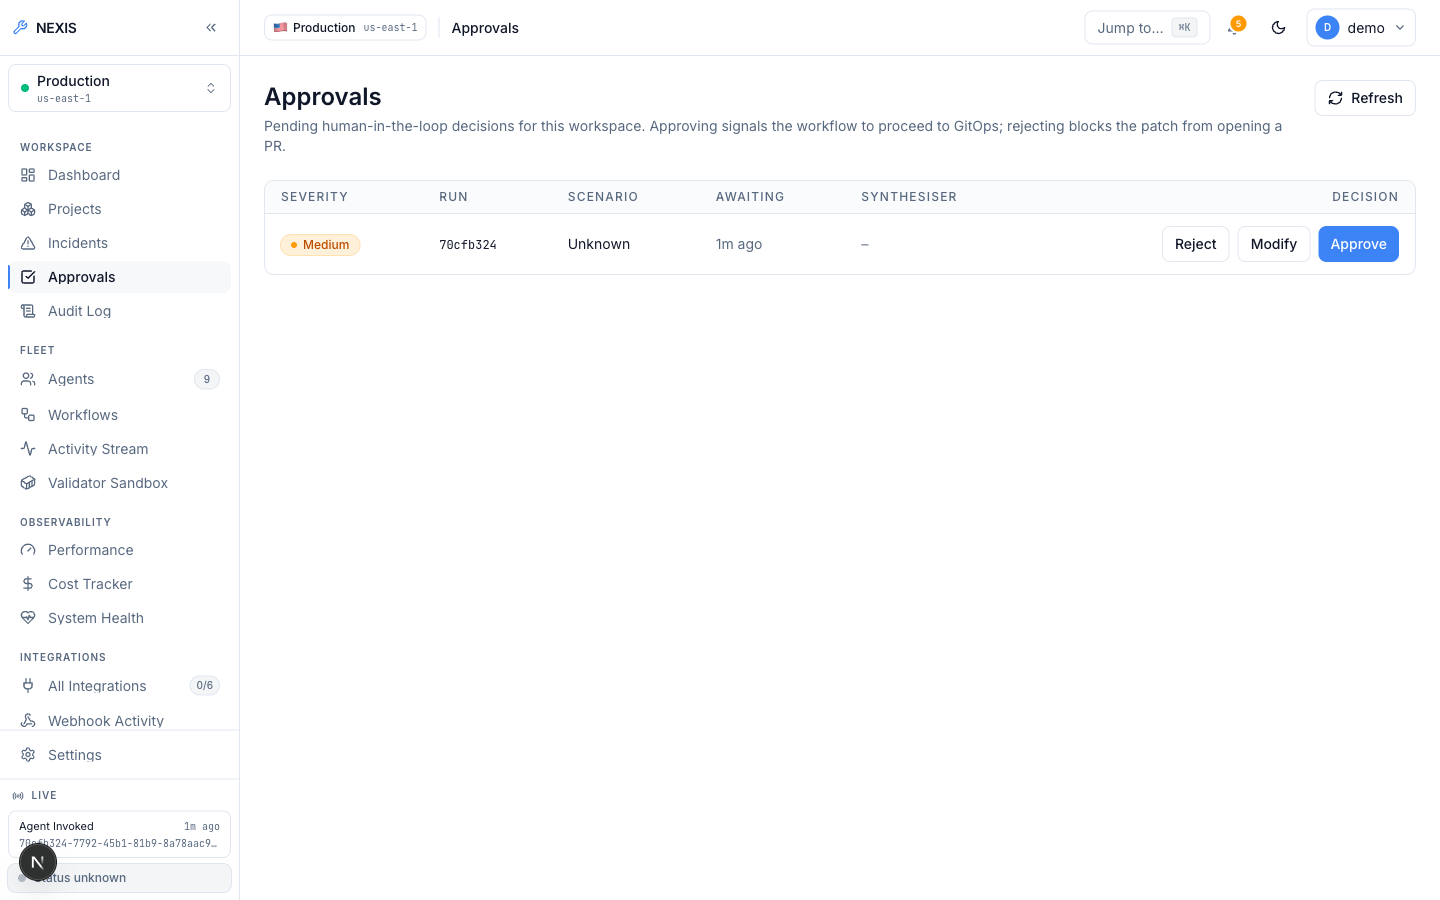
\includegraphics[width=0.85\textwidth]{../assets/screenshots/10-approvals.png}
\caption{Approvals Queue ( real pending approval row with Reject / Modify / Approve actions ).}
\label{fig:approvals}
\end{figure}

The Modify action opens the dialog in Figure~\ref{fig:modifydialog}. This is
the RLHF mechanism described in Chapter~4 made concrete: the engineer edits
the LLM-generated unified diff directly in the embedded editor before
approving, and the edited diff --- along with every other terminal approval
decision --- is persisted as a row in the \code{feedback\_examples} table.
Those rows feed a JSONL export endpoint intended for future fine-tuning;
actually submitting a paid fine-tuning job against the exported data is a
deliberate manual step, not an automated one.

\begin{figure}[htbp]\centering
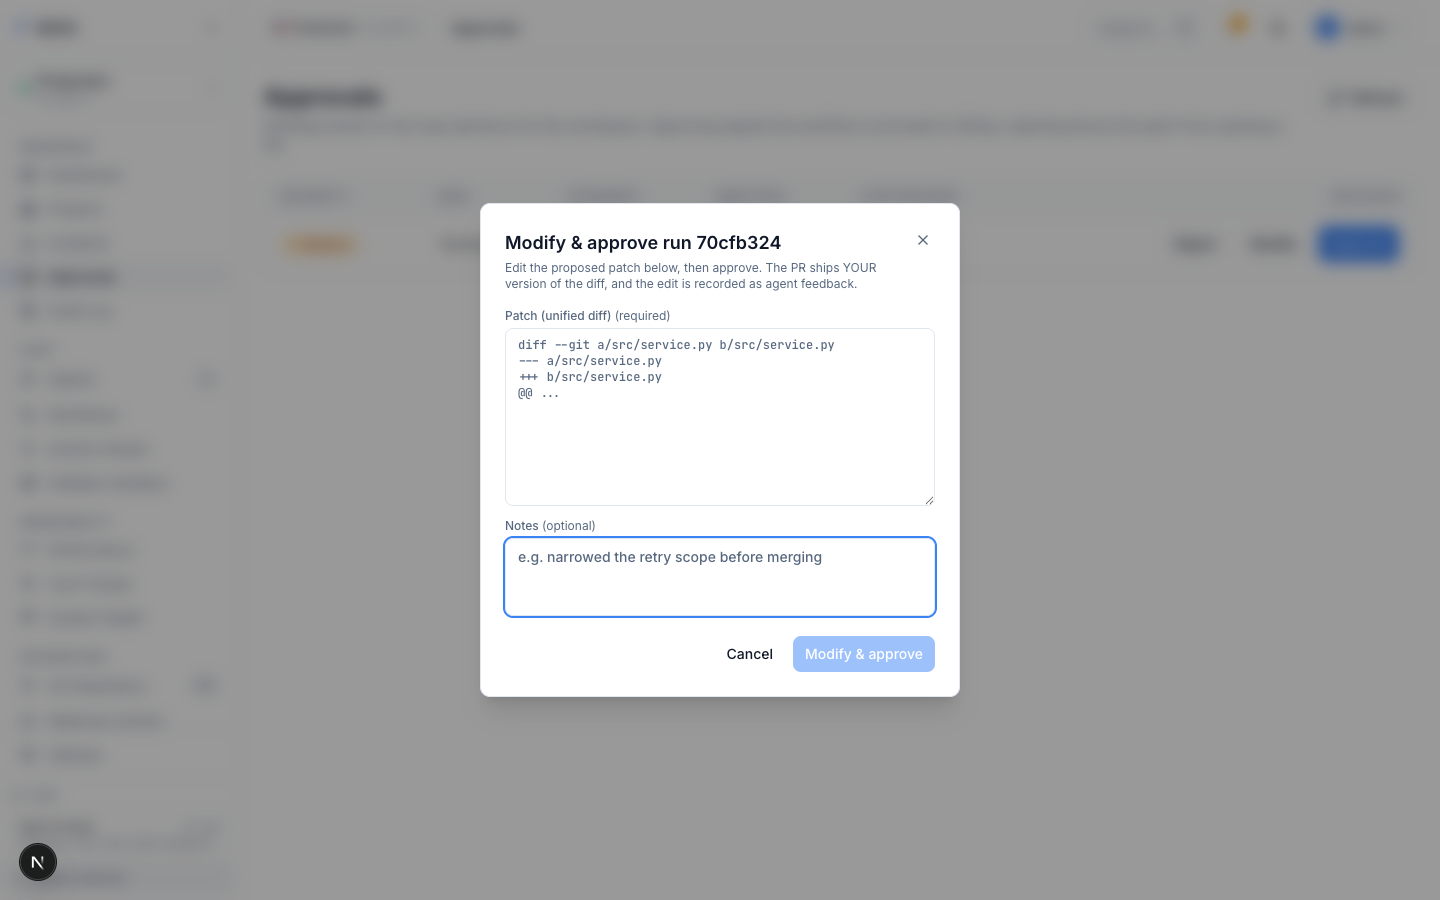
\includegraphics[width=0.85\textwidth]{../assets/screenshots/37-approval-modify-dialog.png}
\caption{Modify-and-Approve Dialog ( RLHF diff editing; the engineer's edit becomes a feedback\_examples training row ).}
\label{fig:modifydialog}
\end{figure}

Figure~\ref{fig:timeoutrun} is an honest negative result, reported
deliberately. For this first run, the 120-second approval window elapsed
before a decision was recorded, and the workflow terminated the run as
\code{timeout\_rejected}. This is the timeout safety mechanism working
exactly as designed: when no human decision arrives in time, the system's
default is to refuse to deploy unreviewed code, not to proceed. A pipeline
that silently auto-deployed on timeout would be a defect; this behaviour is
the intended safe failure mode.

\begin{figure}[htbp]\centering
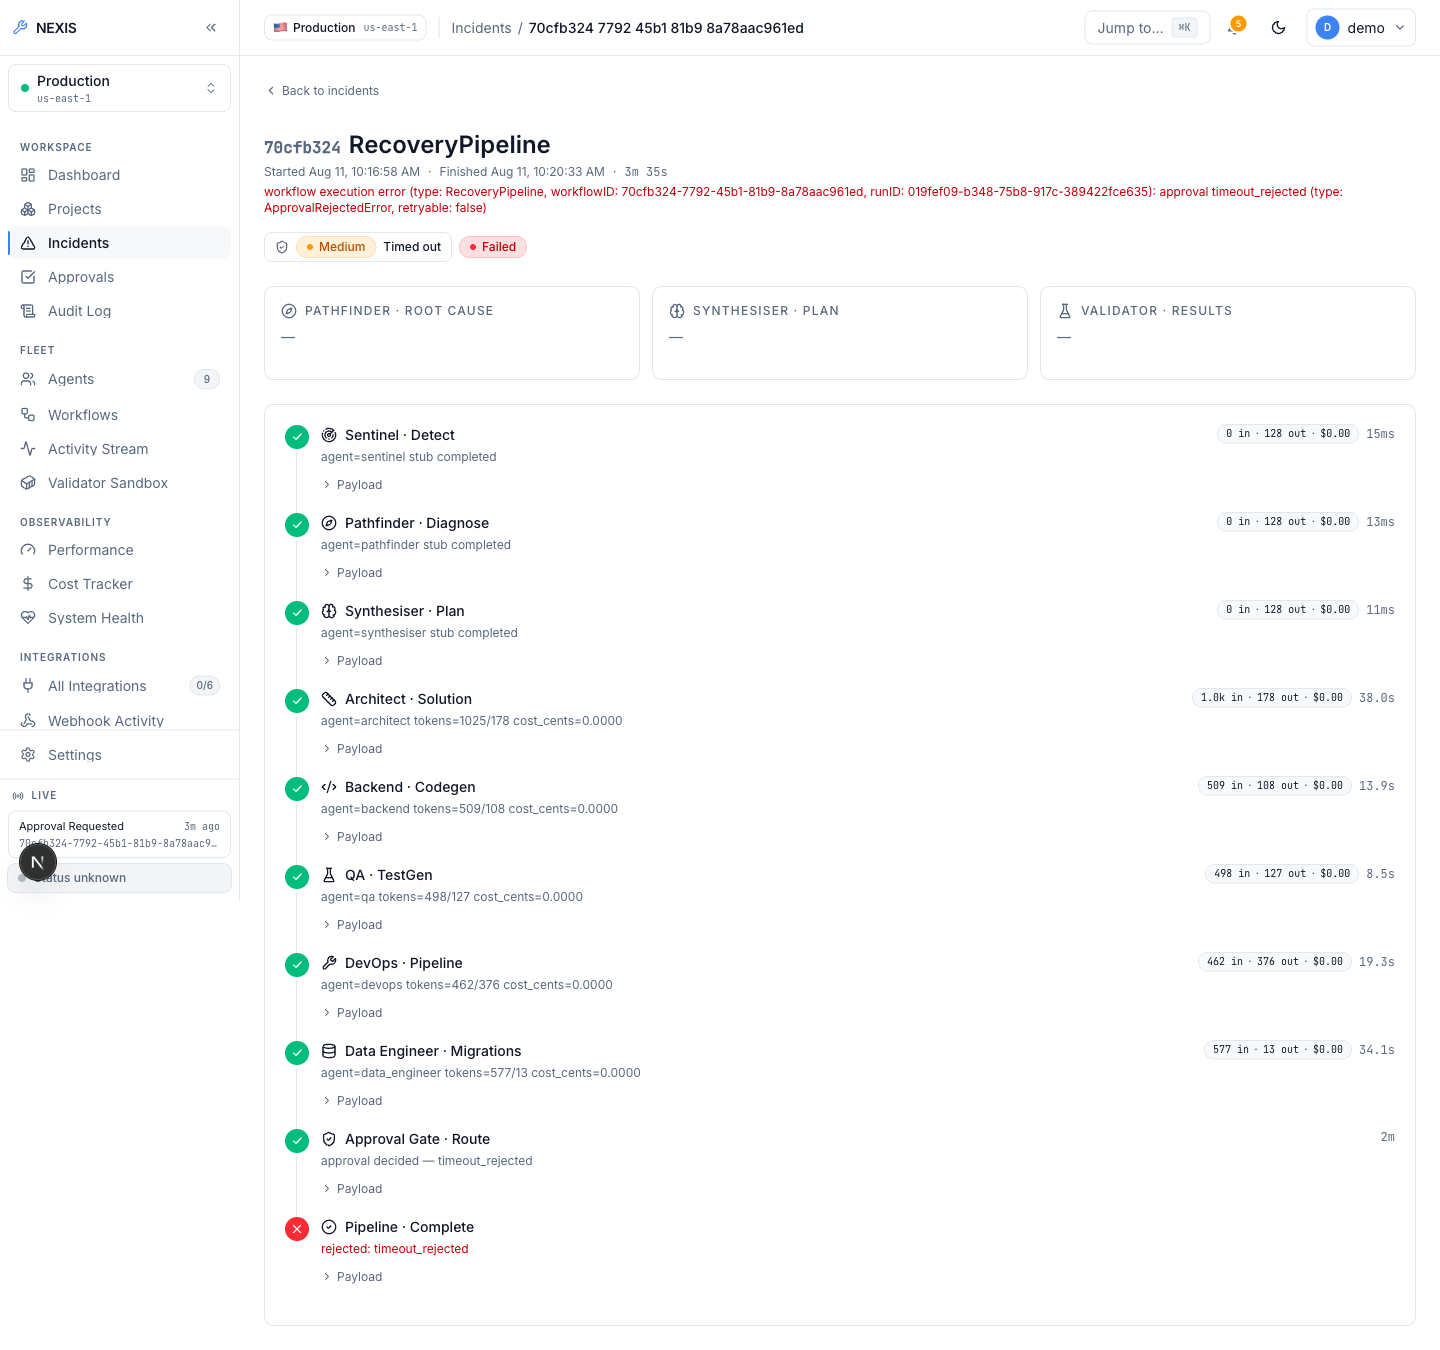
\includegraphics[width=0.85\textwidth]{../assets/screenshots/39-incident-approved-final.png}
\caption{Timeout-Rejected Run ( the 120-second approval window elapsed; the workflow safely auto-rejected as timeout\_rejected rather than deploying unreviewed code ).}
\label{fig:timeoutrun}
\end{figure}

Figure~\ref{fig:fullsuccess} is the key positive result of this report: a
second live run, approved by a human within the window. The incident shows
severity ``Medium'', decision ``Approved'', and outcome ``Succeeded'', with
the full nine-step timeline --- detection through plan, patch generation,
test generation, validation, approval, and deployment steps --- completing
in 1\,minute 40\,seconds end-to-end, with real per-agent token and cost
figures throughout.

\begin{figure}[htbp]\centering
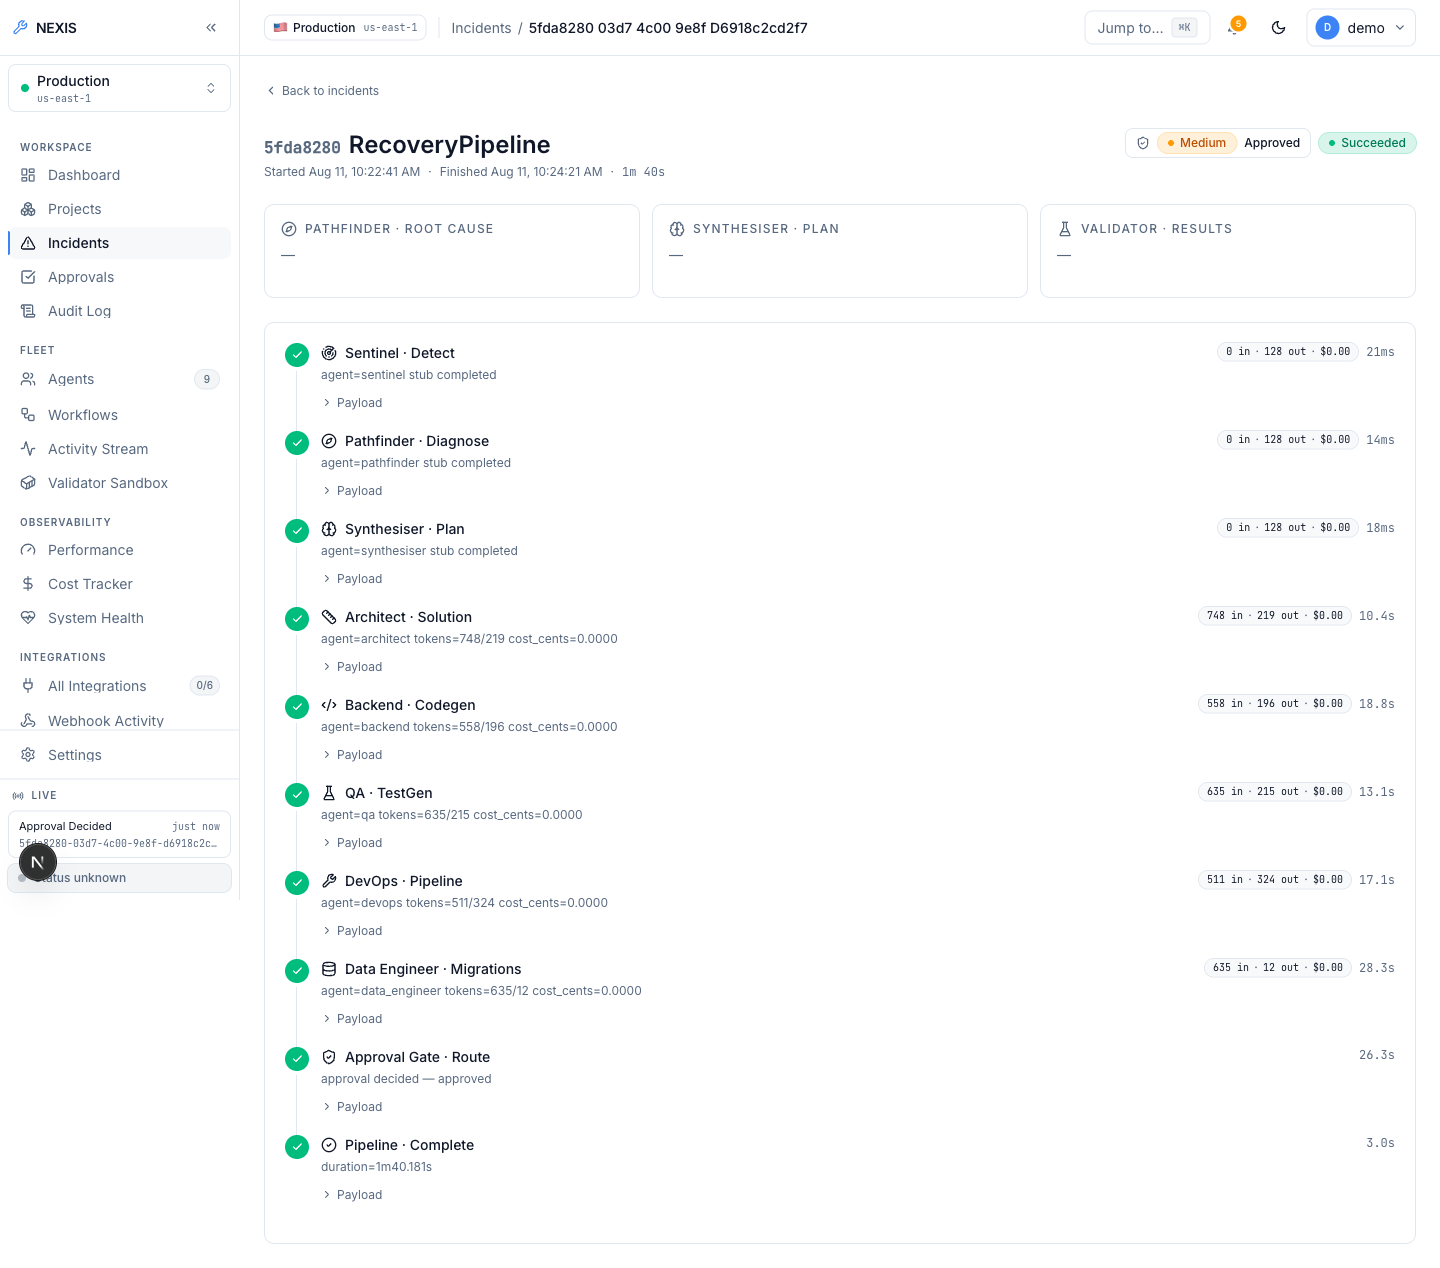
\includegraphics[width=0.85\textwidth]{../assets/screenshots/40-incident-full-success.png}
\caption{Fully Approved Run ( Medium severity, Approved, Succeeded; complete nine-step timeline in 1\,m\,40\,s with real per-agent token and cost figures ).}
\label{fig:fullsuccess}
\end{figure}

Finally, Figure~\ref{fig:payload} settles the question of whether the patch
itself is genuinely LLM-generated. It shows the expanded raw JSON payload of
the Backend agent's step: the actual unified diff produced by
\code{qwen2.5-coder:14b}, with \code{provider="ollama"} recorded in the
payload. The patch is model output parsed from a unified diff, not a
template retrieved from a fixture.

\begin{figure}[htbp]\centering
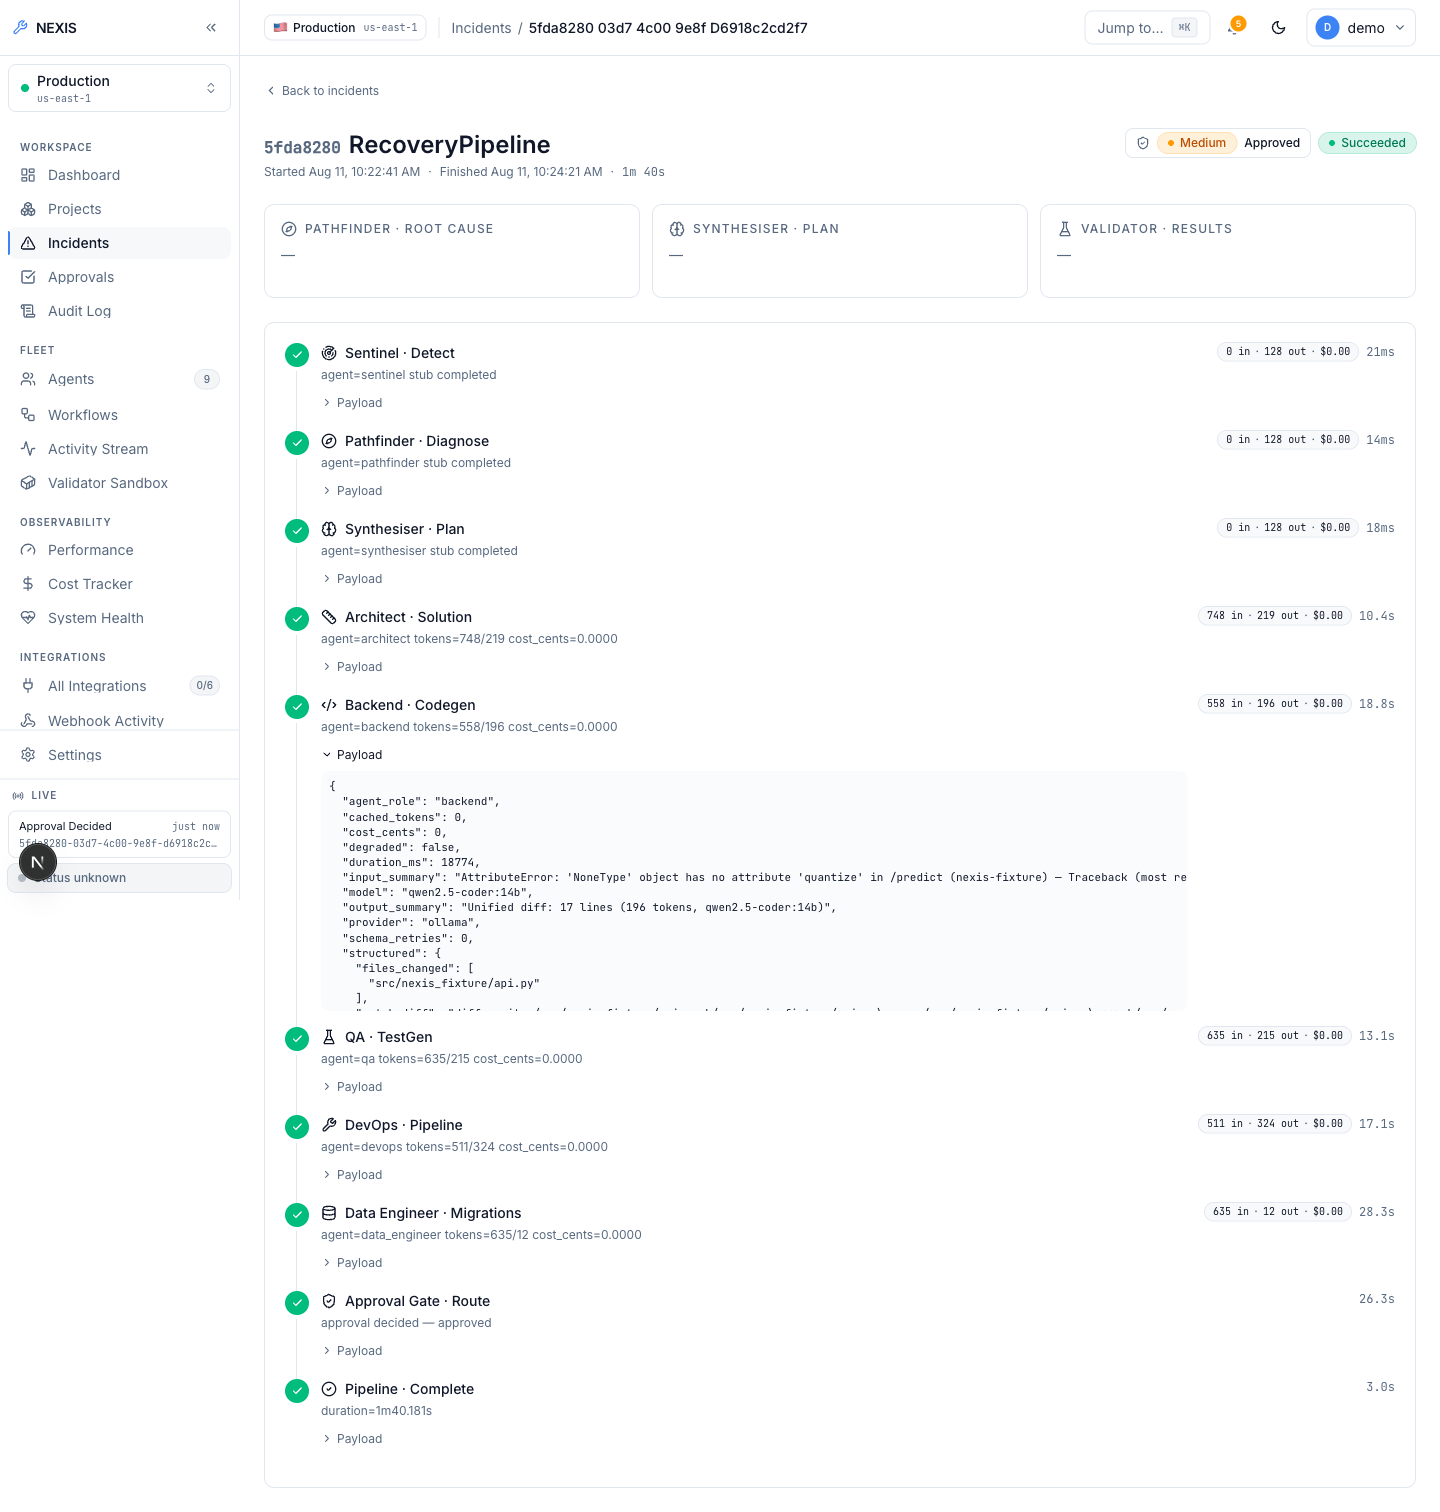
\includegraphics[width=0.85\textwidth]{../assets/screenshots/41-backend-payload-expanded.png}
\caption{Backend Payload, Expanded ( raw JSON evidence of the qwen2.5-coder:14b-generated unified diff, provider=``ollama'' ).}
\label{fig:payload}
\end{figure}

\subsection{Docker Preview-Deploy Engine (Ops Tab)}
\label{sec:opstab}

Each project detail page is organised into tabs. The Overview tab
(Figure~\ref{fig:projoverview}) summarises the project; Integrations
(Figure~\ref{fig:projintegrations}) manages the project's provider
connections, most importantly the GitHub repository binding; Recovery Policy
(Figure~\ref{fig:projpolicy}) configures per-project self-healing behaviour
such as rollback-on-SLO-breach; and Activity (Figure~\ref{fig:projactivity})
shows the project-scoped event history.

\begin{figure}[htbp]\centering
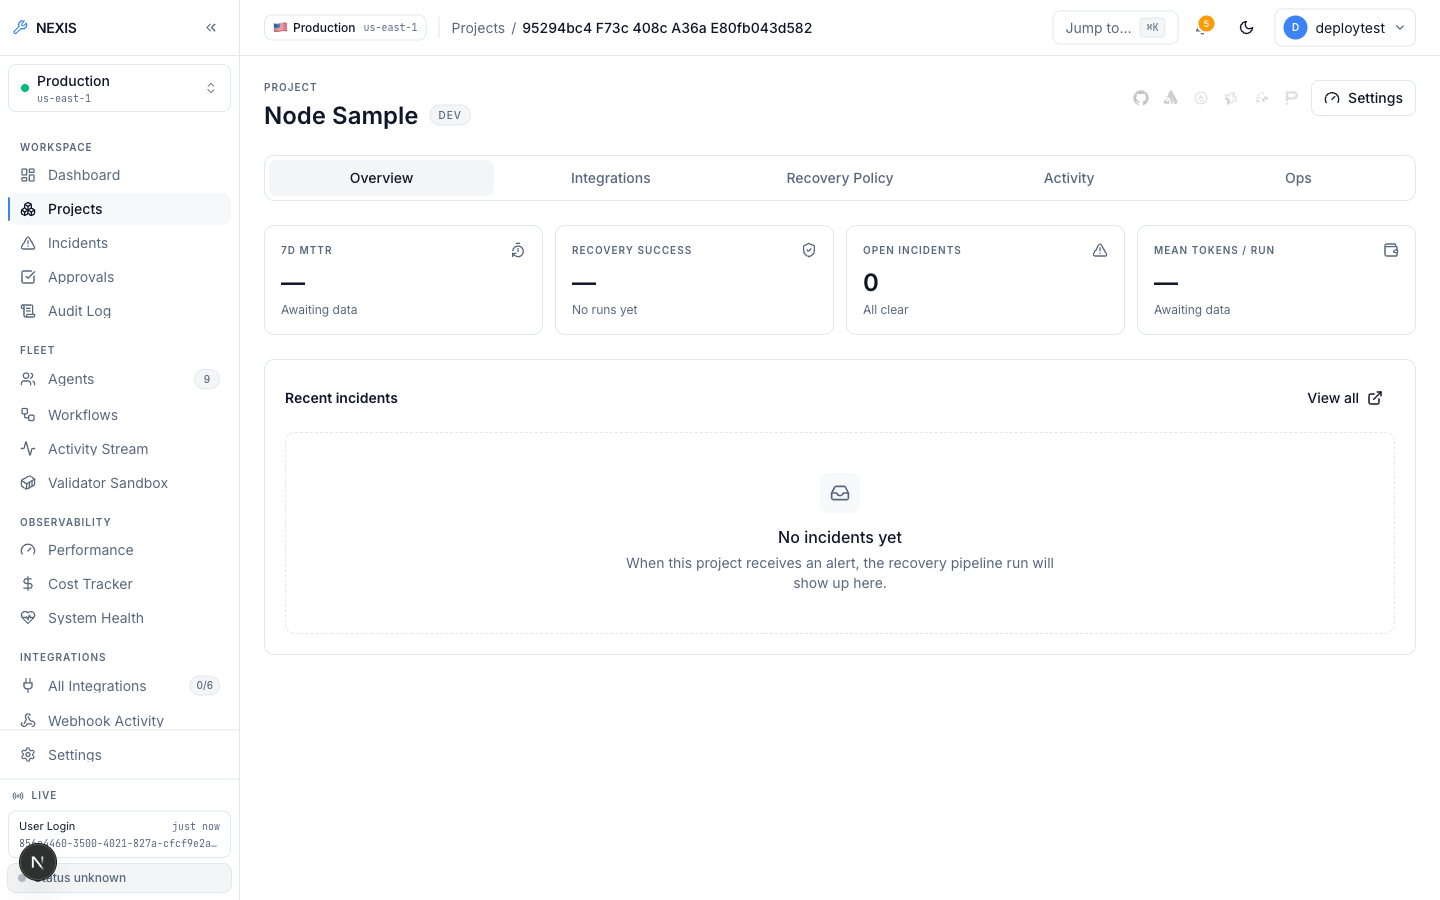
\includegraphics[width=0.85\textwidth]{../assets/screenshots/28-project-overview.png}
\caption{Project Overview Tab ( project summary and health ).}
\label{fig:projoverview}
\end{figure}

\begin{figure}[htbp]\centering
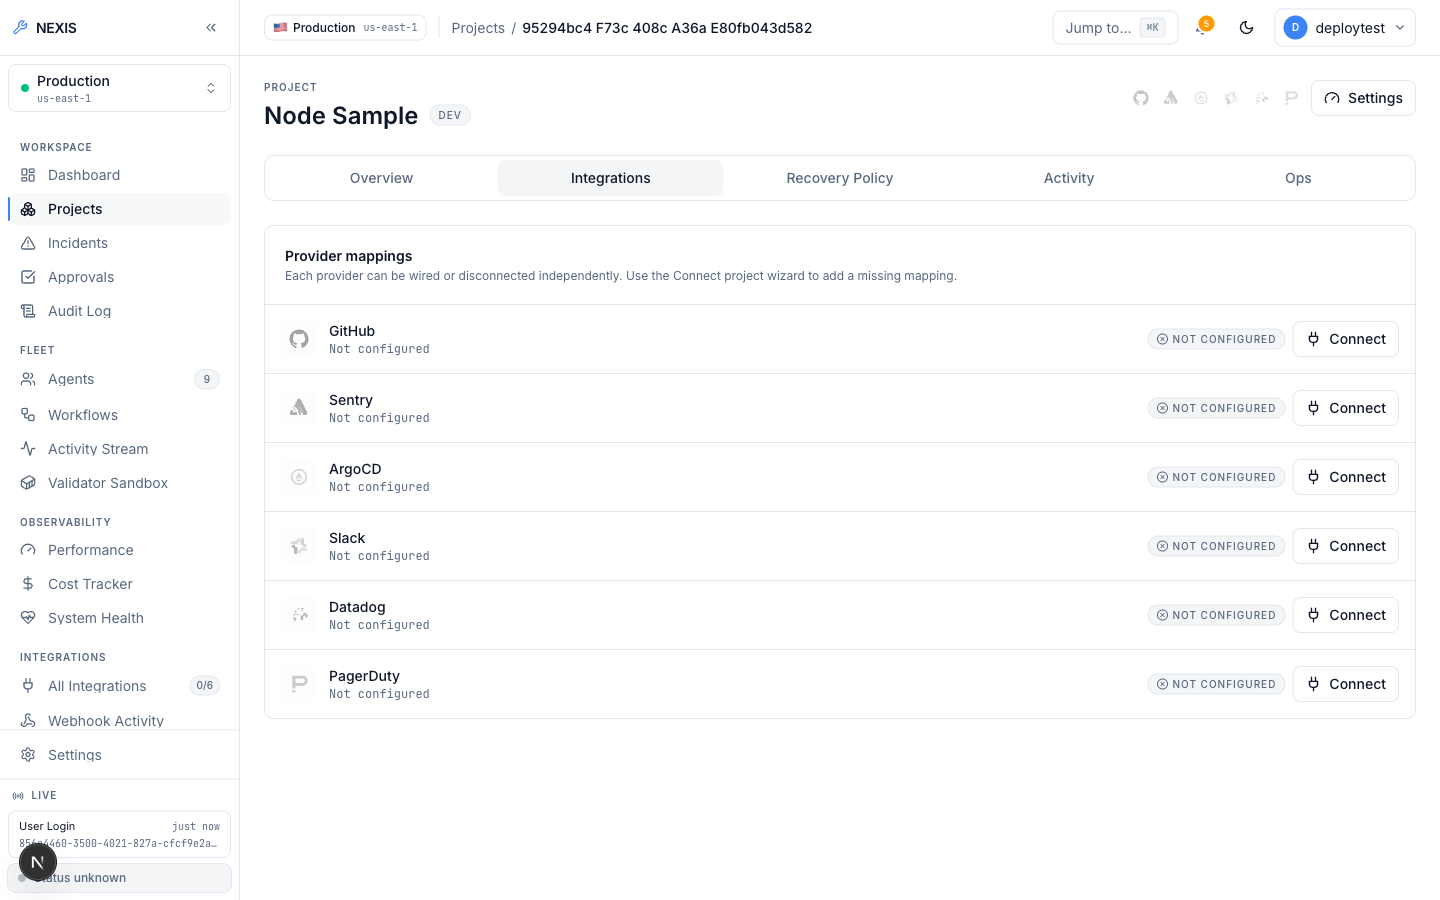
\includegraphics[width=0.85\textwidth]{../assets/screenshots/29-project-integrations.png}
\caption{Project Integrations Tab ( provider connections including the GitHub repository binding ).}
\label{fig:projintegrations}
\end{figure}

\begin{figure}[htbp]\centering
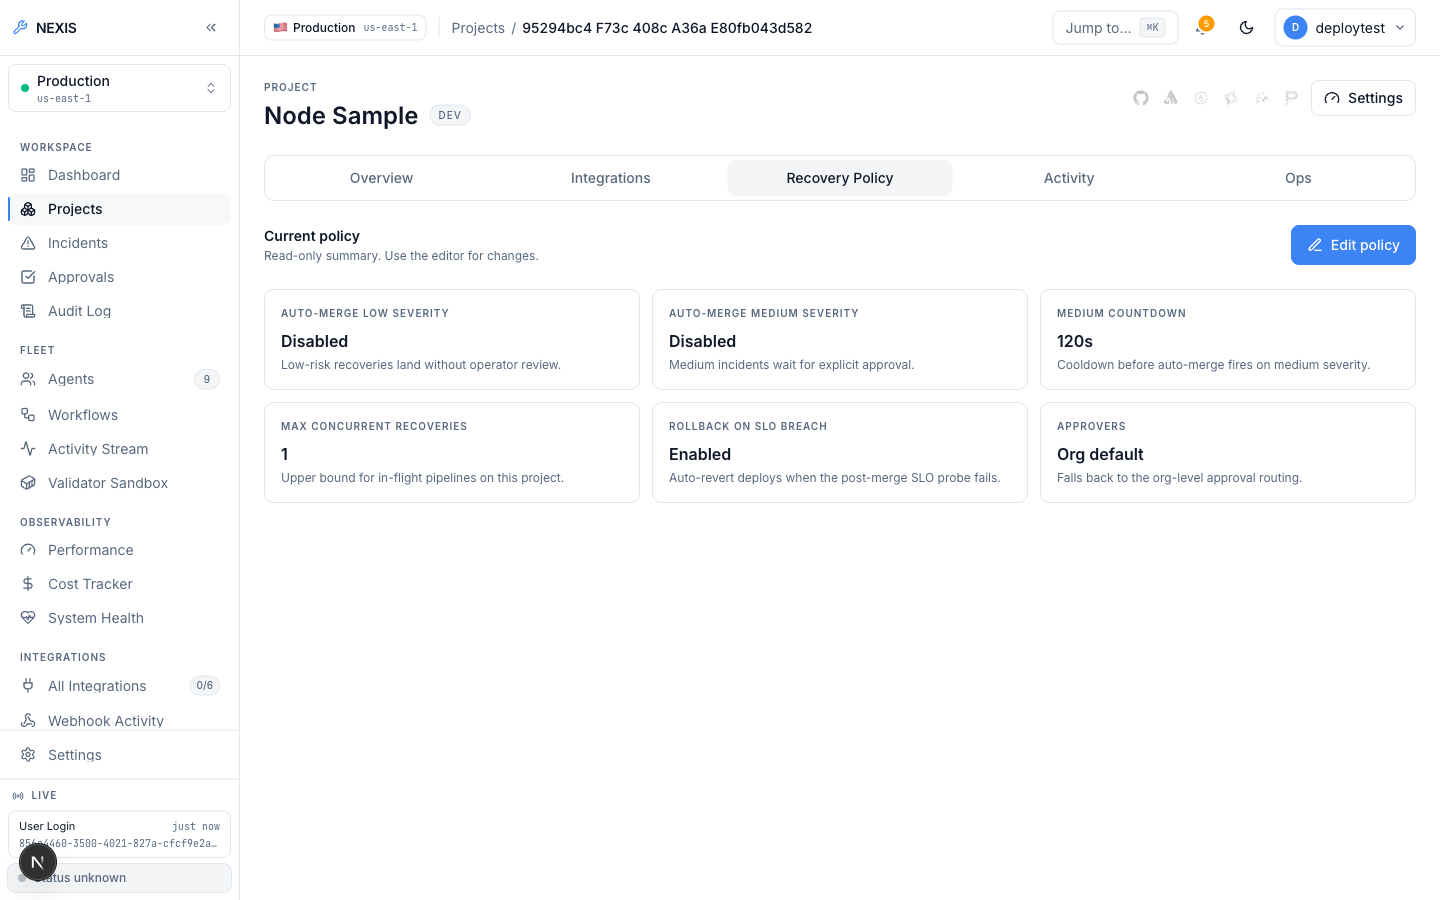
\includegraphics[width=0.85\textwidth]{../assets/screenshots/30-project-recovery-policy.png}
\caption{Project Recovery Policy Tab ( per-project self-healing configuration ).}
\label{fig:projpolicy}
\end{figure}

\begin{figure}[htbp]\centering
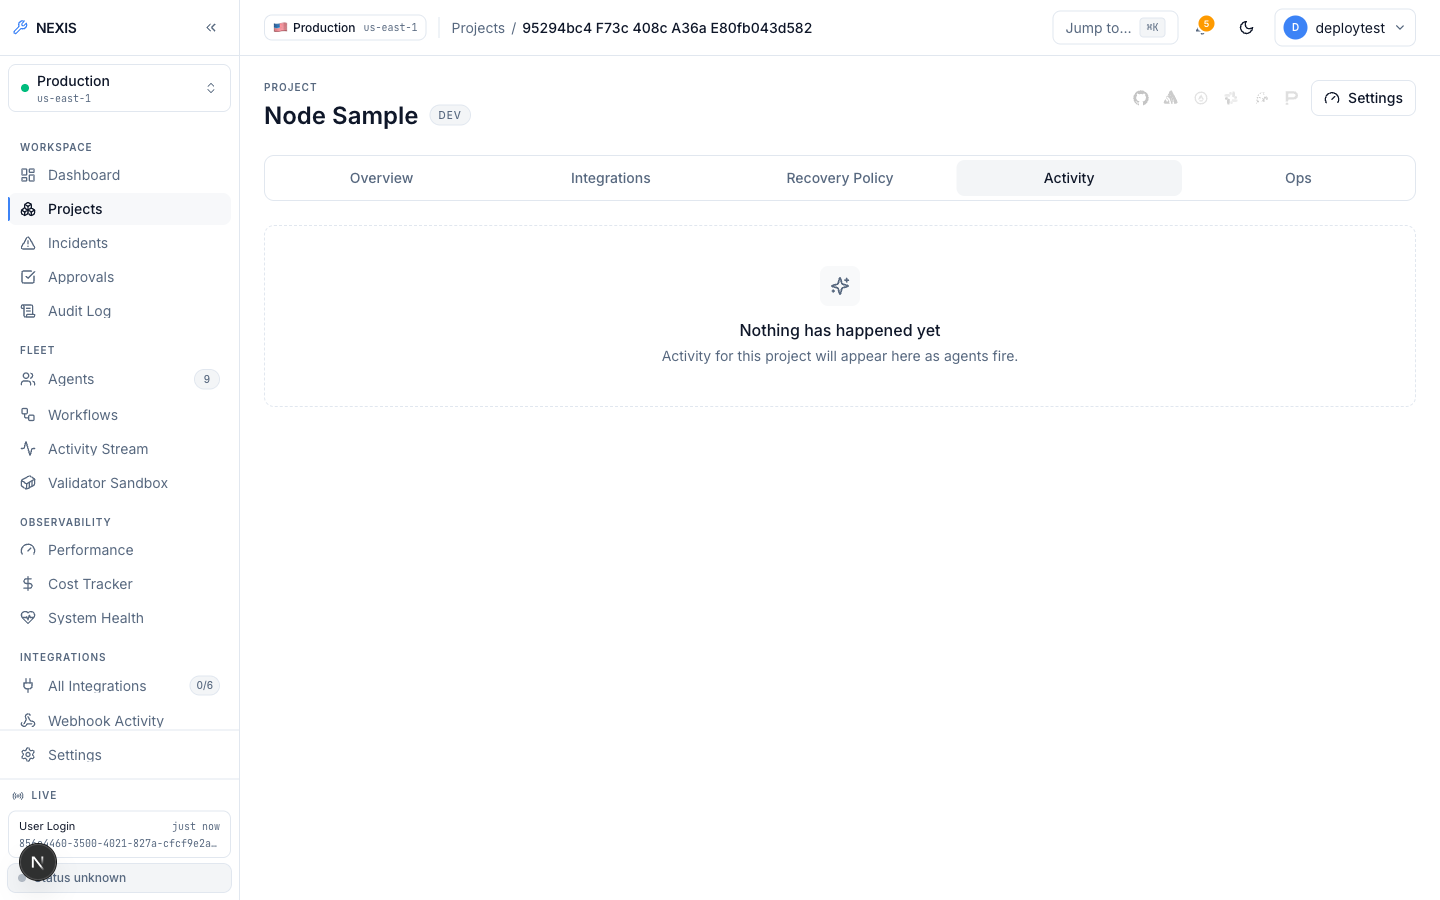
\includegraphics[width=0.85\textwidth]{../assets/screenshots/31-project-activity.png}
\caption{Project Activity Tab ( project-scoped event history ).}
\label{fig:projactivity}
\end{figure}

The Ops tab is the frontend to the preview-deploy engine.
Figure~\ref{fig:opsempty} shows its empty state before any deployment: the
Deploy action, live status area, and (once populated) the preview URL,
build/container logs, and deployment history.

\begin{figure}[htbp]\centering
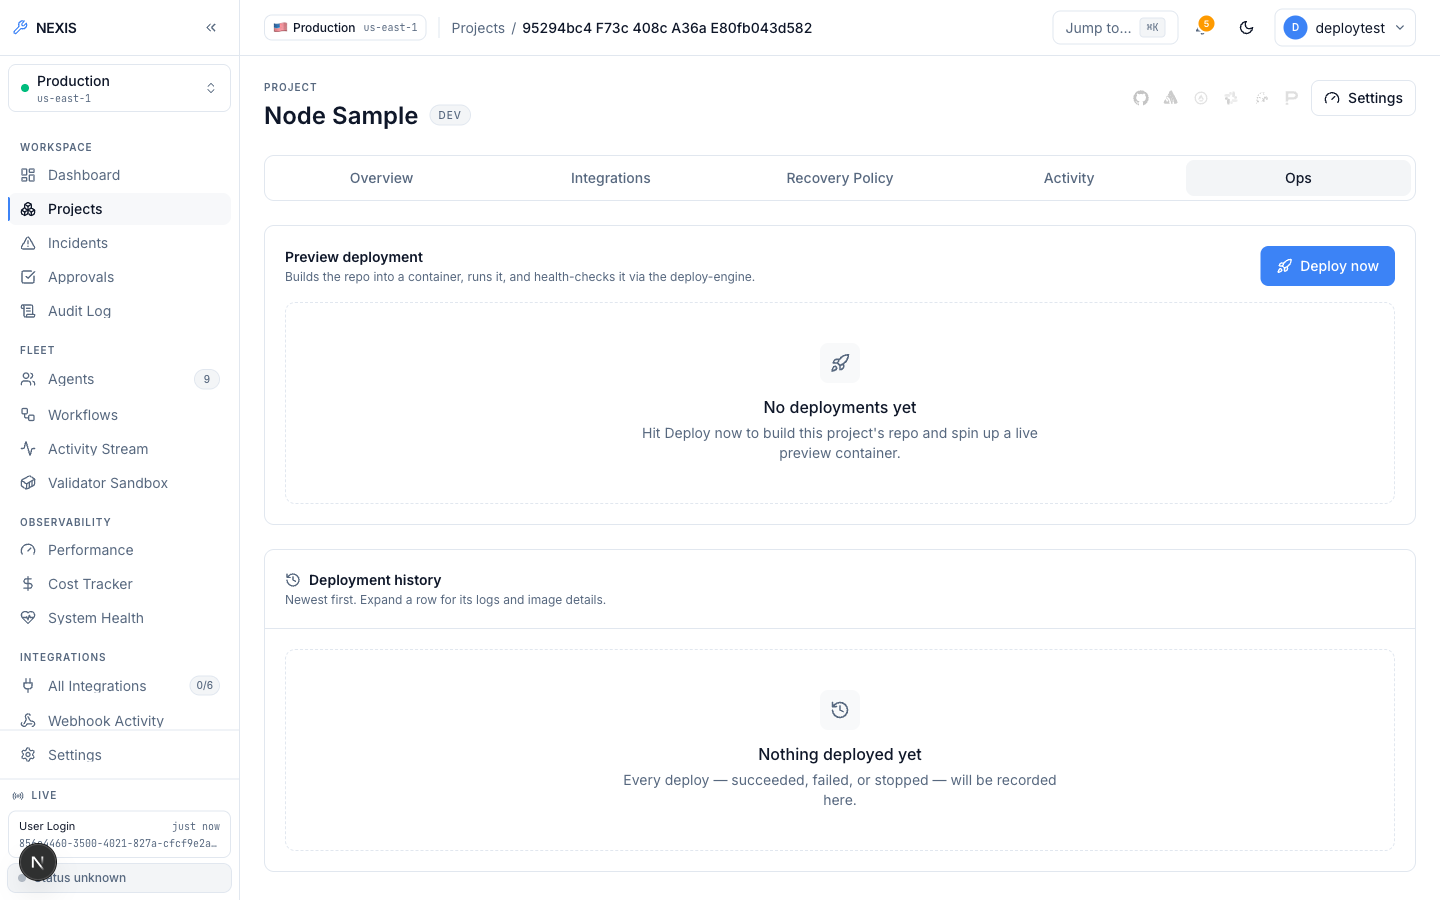
\includegraphics[width=0.85\textwidth]{../assets/screenshots/32-project-ops-empty.png}
\caption{Project Ops Tab, Empty State ( the Deploy panel before any deployment ).}
\label{fig:opsempty}
\end{figure}

Figure~\ref{fig:opsattempt} shows what happened when Deploy was clicked on a
project with no GitHub App connection in the evaluation environment: the
real API returned the validation error ``project has no github repository
bound'', which the UI surfaces verbatim. To be clear, this capture does
\emph{not} show a successful deploy --- it shows the real validation chain
rejecting a deploy request that cannot be fulfilled, which is the correct
behaviour. The limitation here is environmental (no GitHub App credentials
exist in the evaluation environment, as stated in Chapter~7's limitations),
not a defect in the engine.

\begin{figure}[htbp]\centering
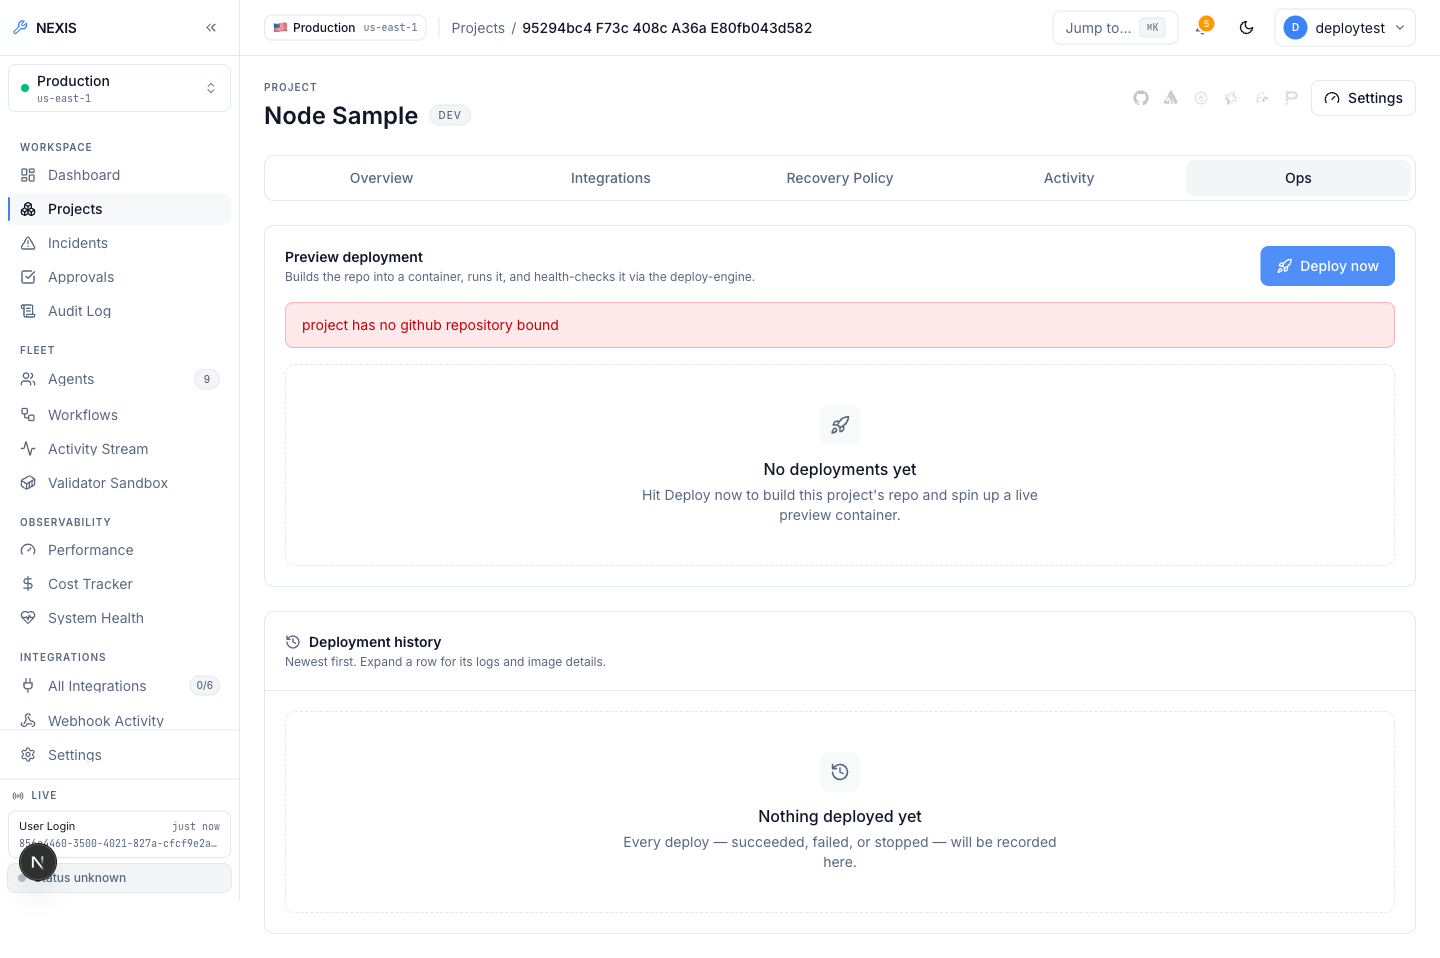
\includegraphics[width=0.85\textwidth]{../assets/screenshots/33-project-ops-deploy-attempt.png}
\caption{Project Ops Tab, Deploy Attempt ( a real validation error --- ``project has no github repository bound'' --- returned by the live API ).}
\label{fig:opsattempt}
\end{figure}

The engine itself, however, was proven live independently of that credential
limitation. Listing~\ref{lst:deployrun} reproduces verbatim the verified
end-to-end run recorded during this project: a real public repository
(\code{heroku/node-js-getting-started}, which contains no Dockerfile) was
cloned, its stack was detected as Node from marker files, a working
Dockerfile was generated, the image was built, the container was run under
resource limits, and an HTTP request to the returned preview URL served the
application's real rendered HTML page. The container was then stopped and
removed cleanly.

\begin{lstlisting}[caption={Verified live deploy-engine run},label={lst:deployrun}]
POST /v1/deploy  (repo: heroku/node-js-getting-started, no Dockerfile present)
-> 200 OK
  "status": "running", "dockerfile_source": "generated", "detected_stack": "node",
  "url": "http://localhost:54671", "image_tag": "nexis-preview-test-project:22d06076c357"
  build_log: "...npm ci... EXPOSE 3000... CMD [\"npm\",\"start\"]..."
  container_log: "Listening on 3000\nRendering 'pages/index' for route '/'"

GET http://localhost:54671/  -> real rendered HTML of the Node app (verified)

POST /v1/deploy/test-e2e-001/stop -> {"status":"stopped"}; container removed.
\end{lstlisting}

When a build or health check fails, the control plane inserts a real
incident with \code{source: "deploy\_engine"} into the same
Sentinel-to-RecoveryPipeline path used by every other incident source, so a
broken build or an unrecognised stack becomes a self-healing target like any
production fault.

\subsection{Projects, Agents, and Observability}

The Projects page (Figure~\ref{fig:projects}) lists the organisation's
projects as cards; new projects are created through the wizard in
Figure~\ref{fig:newproject}, which derives sensible defaults from the
project name. Each agent has its own detail page ---
Figure~\ref{fig:agentdetail} shows the Backend agent's --- and the Recovery
Pipeline page (Figure~\ref{fig:recoverypipeline}) presents the pipeline
structure itself.

\begin{figure}[htbp]\centering
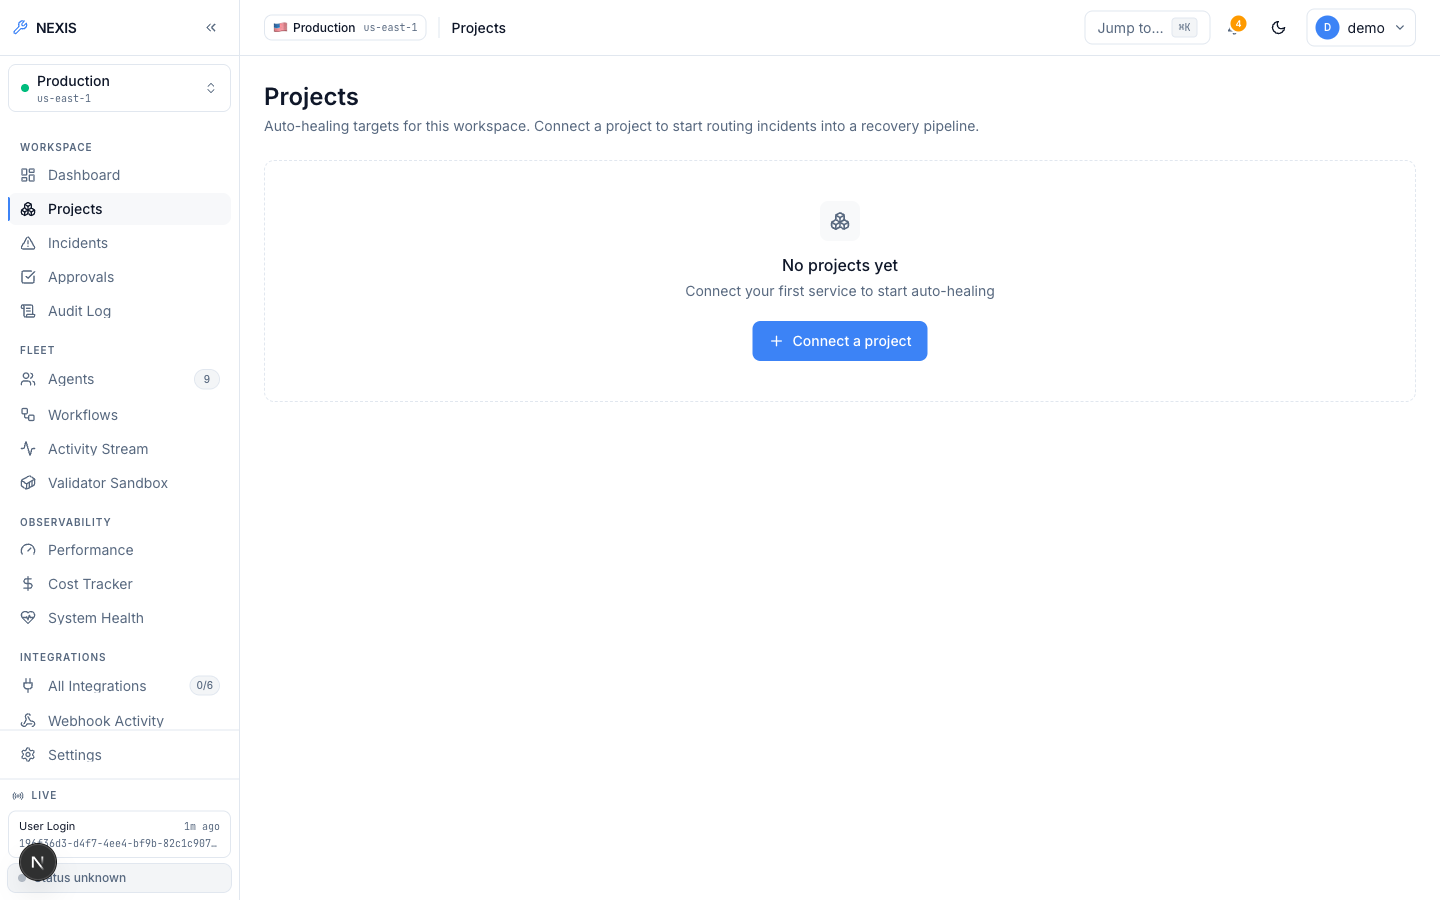
\includegraphics[width=0.85\textwidth]{../assets/screenshots/12-projects.png}
\caption{Projects Screen ( project cards with health indicators ).}
\label{fig:projects}
\end{figure}

\begin{figure}[htbp]\centering
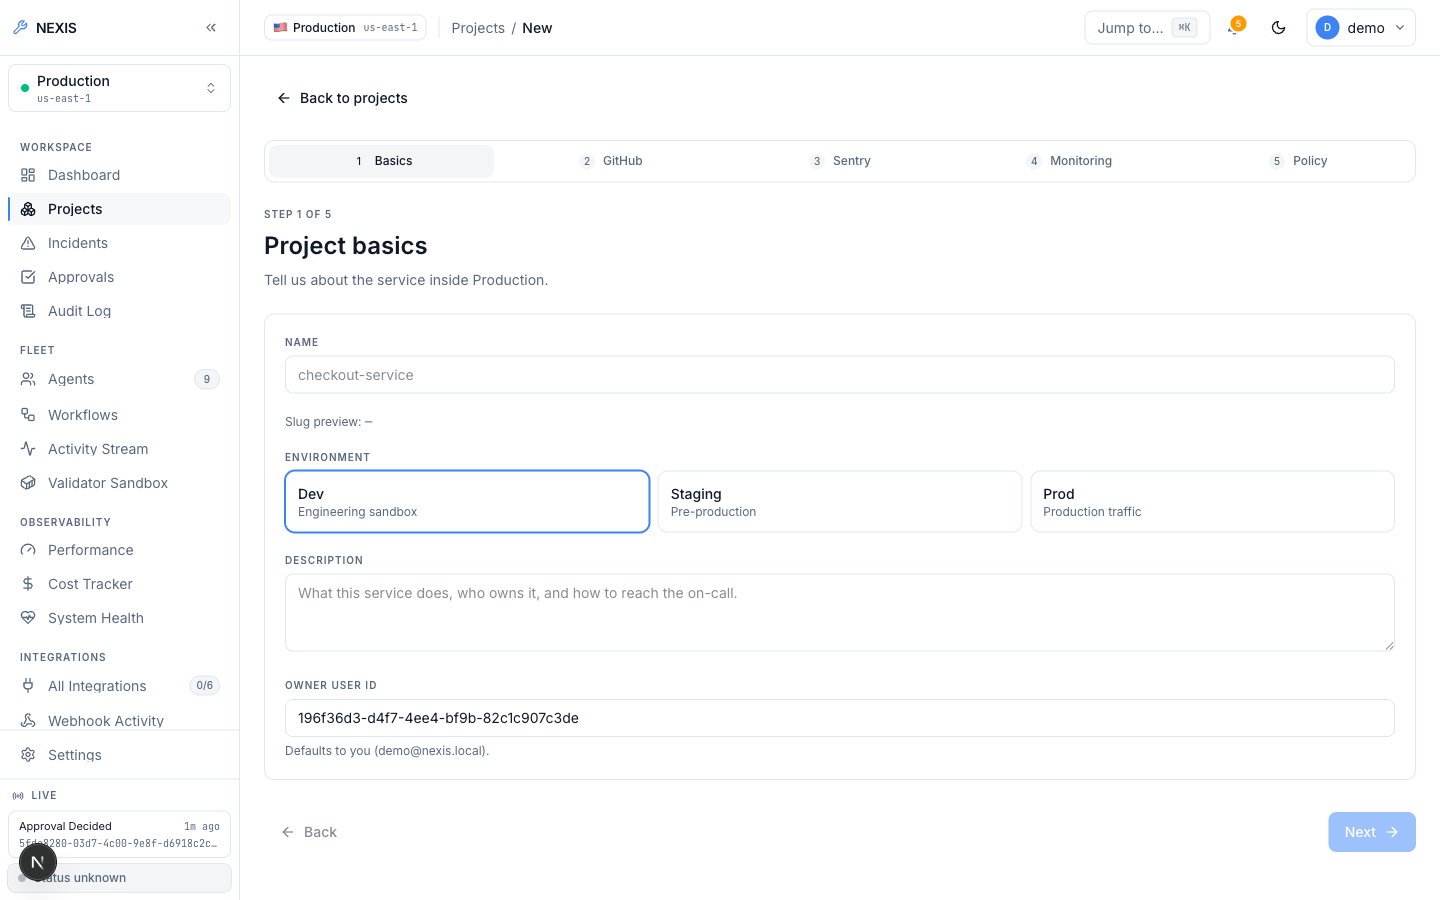
\includegraphics[width=0.85\textwidth]{../assets/screenshots/42-new-project-wizard.png}
\caption{New-Project Wizard ( guided project creation ).}
\label{fig:newproject}
\end{figure}

\begin{figure}[htbp]\centering
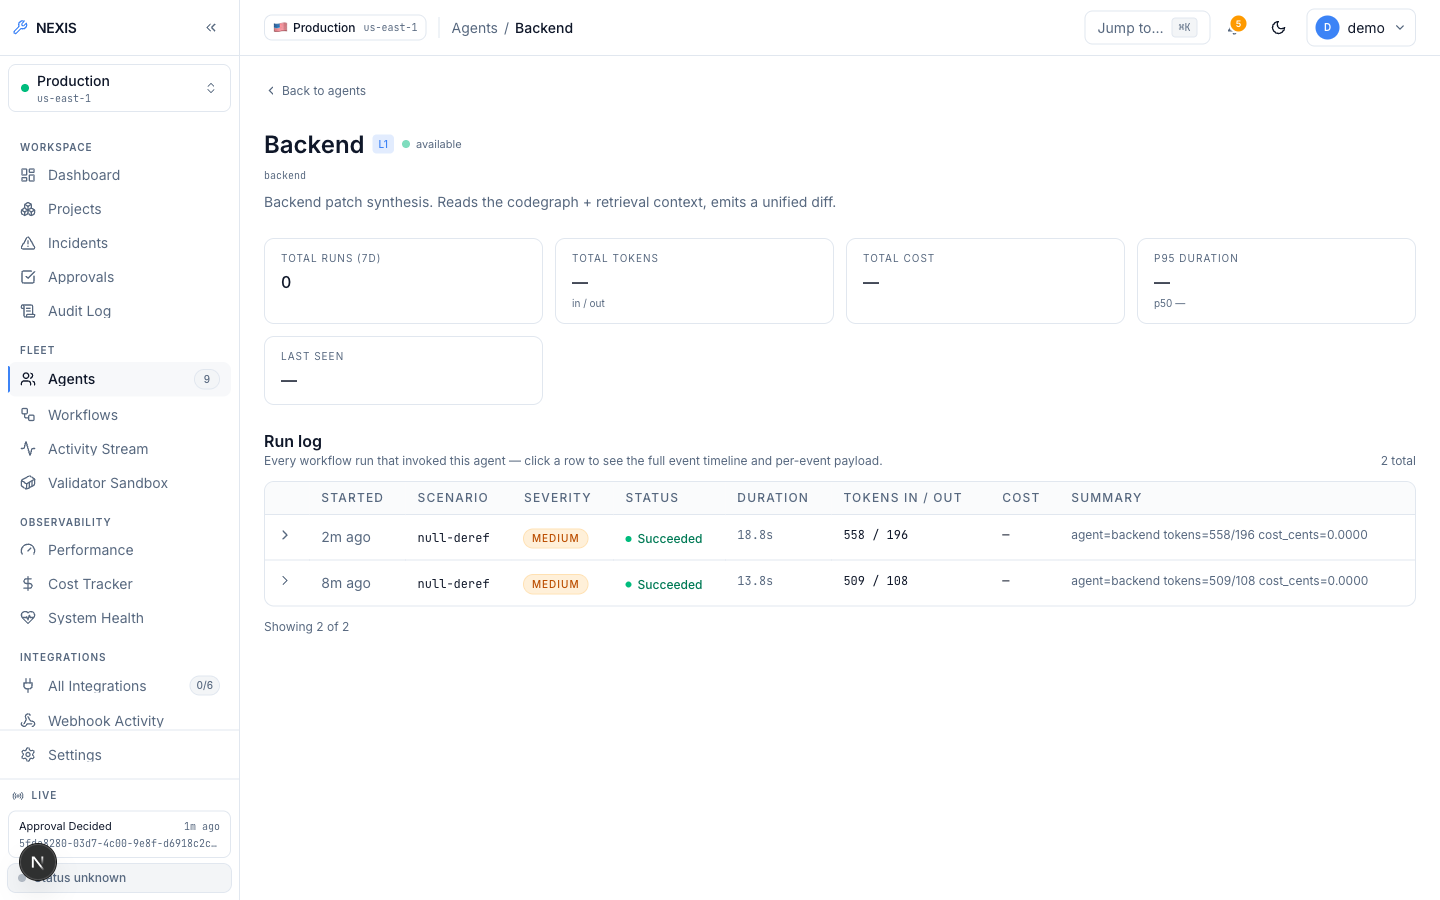
\includegraphics[width=0.85\textwidth]{../assets/screenshots/43-agent-detail-backend.png}
\caption{Agent Detail, Backend Agent ( per-agent configuration and run history ).}
\label{fig:agentdetail}
\end{figure}

\begin{figure}[htbp]\centering
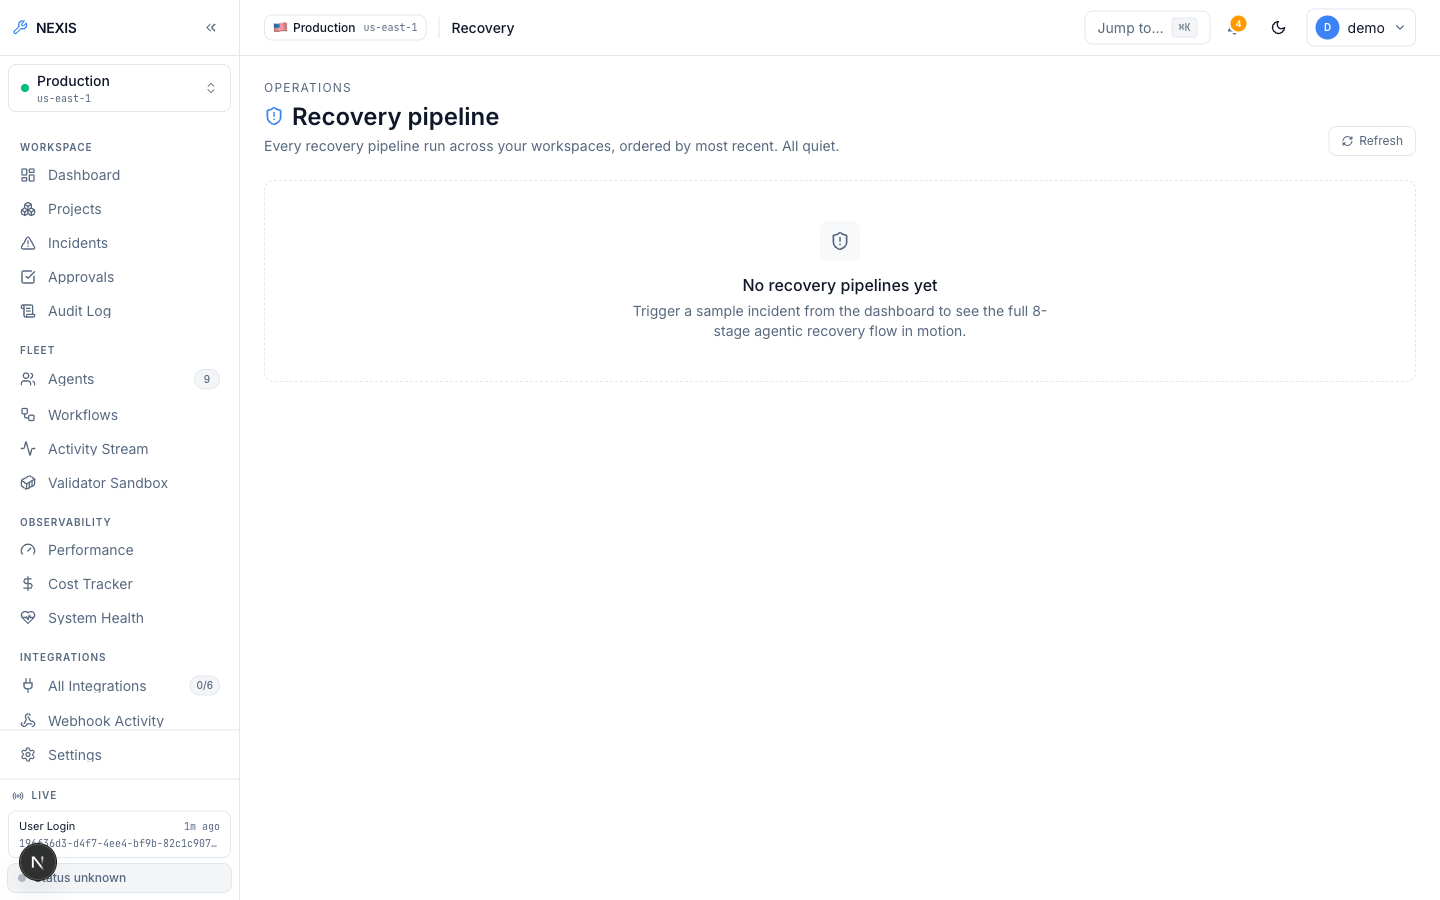
\includegraphics[width=0.85\textwidth]{../assets/screenshots/27-recovery-pipeline.png}
\caption{Recovery Pipeline Screen ( the nine-agent pipeline structure ).}
\label{fig:recoverypipeline}
\end{figure}

Observability is spread across four pages. Performance
(Figure~\ref{fig:performance}) charts pipeline latency and throughput; the
Cost Tracker (Figure~\ref{fig:cost}) rolls up the per-organisation token
ledger against a configurable daily budget; System Health
(Figure~\ref{fig:health}) fans out parallel dependency probes --- Postgres,
Redis, Neo4j, MinIO, Temporal --- under a bounded timeout and reports each
result; and the Eval Harness (Figure~\ref{fig:eval}) runs side-by-side
OpenAI-versus-Ollama provider comparisons across fixture incidents, with
persisted transcripts, cost accounting, and an admin-only CSV export. The
Knowledge Base page (Figure~\ref{fig:kb}) reports the status of the
pgvector-backed retrieval store.

\begin{figure}[htbp]\centering
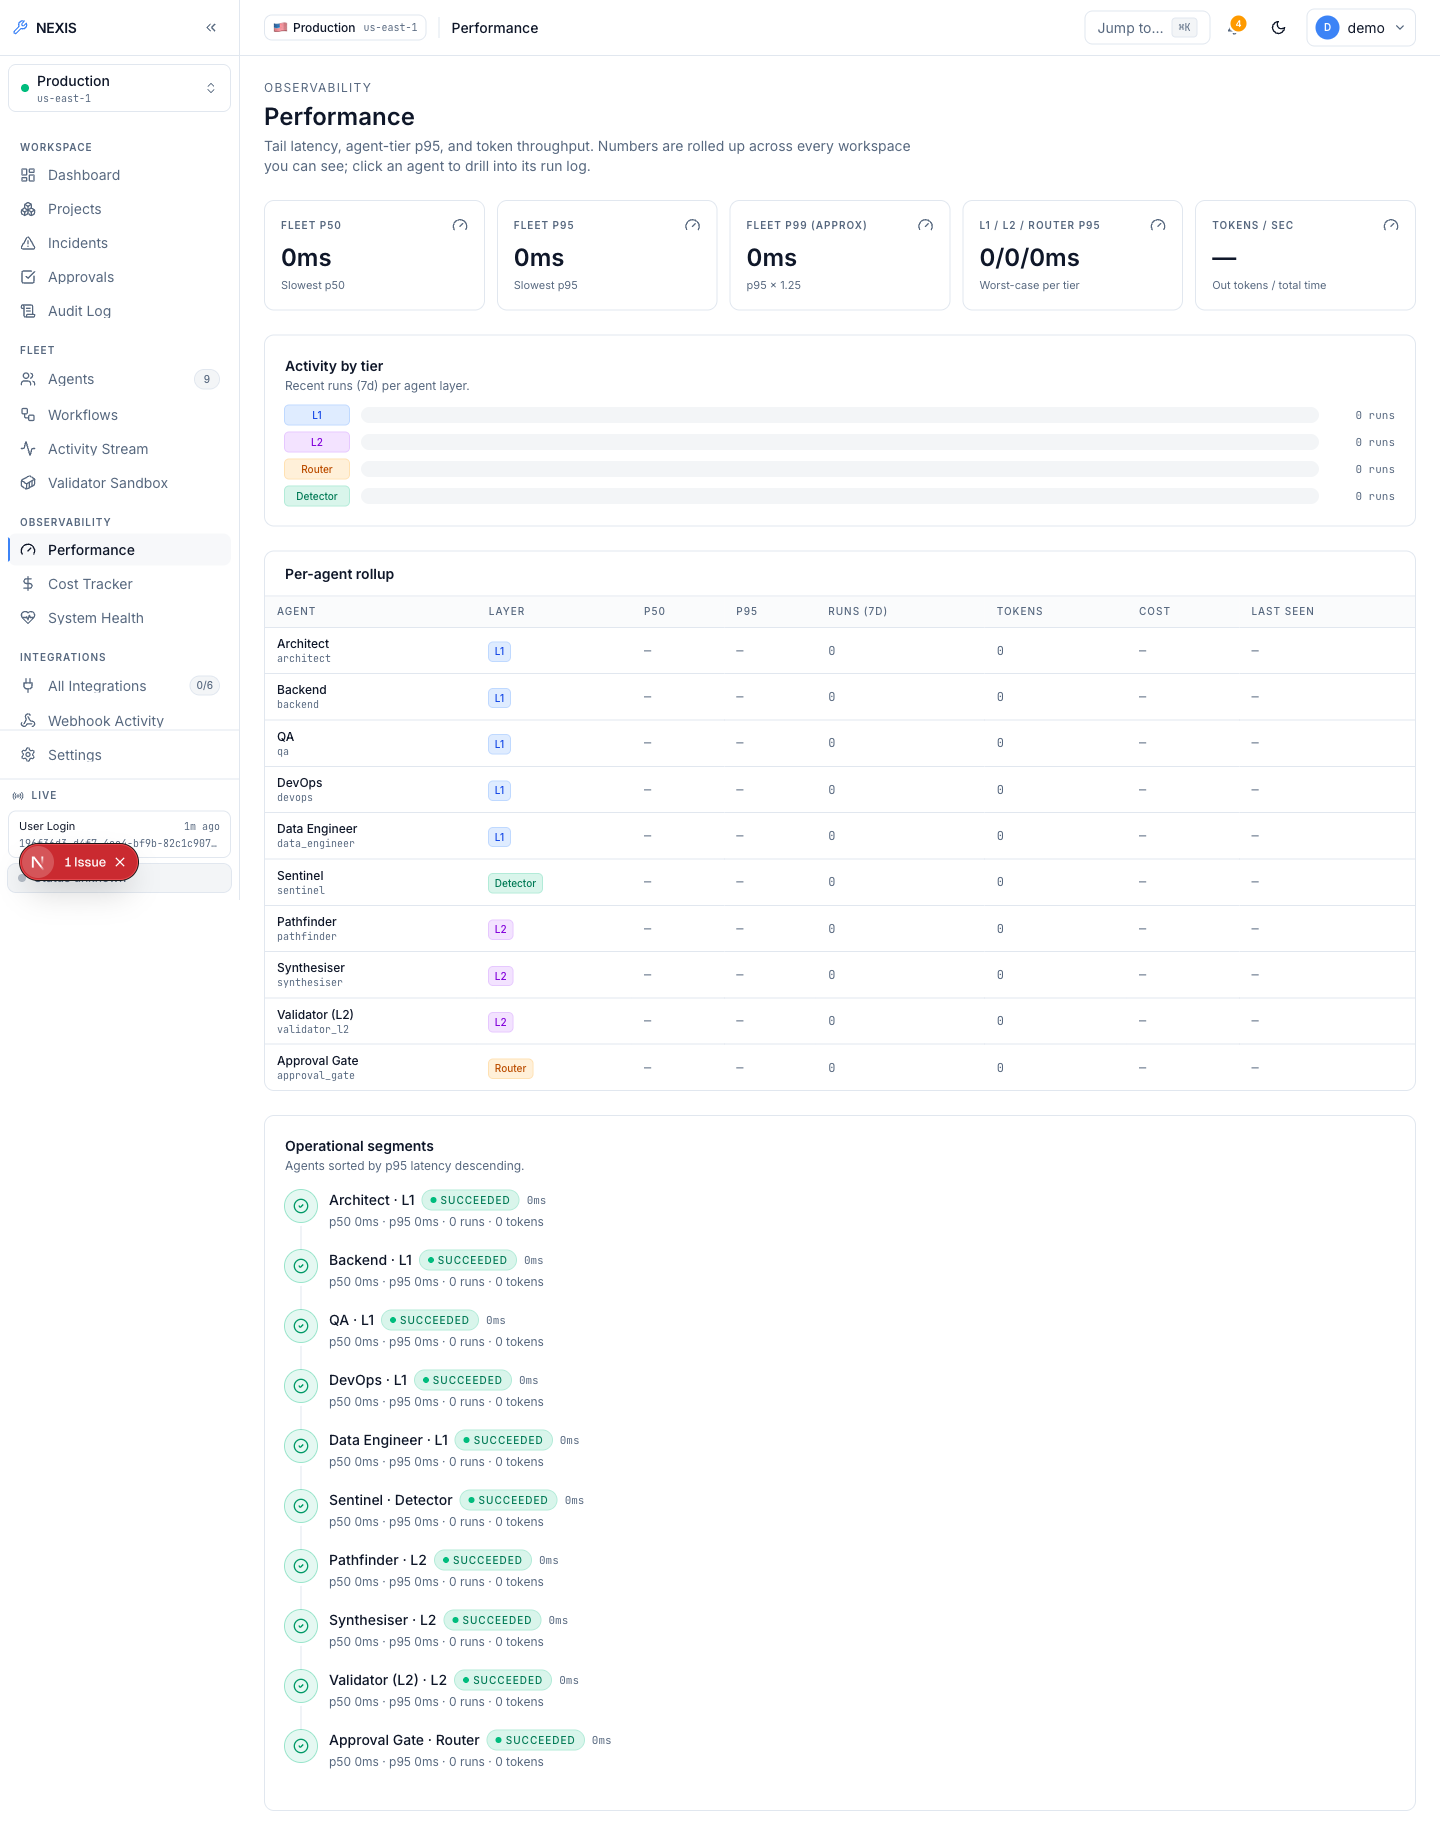
\includegraphics[width=0.85\textwidth]{../assets/screenshots/18-performance.png}
\caption{Performance Screen ( pipeline latency and throughput charts ).}
\label{fig:performance}
\end{figure}

\begin{figure}[htbp]\centering
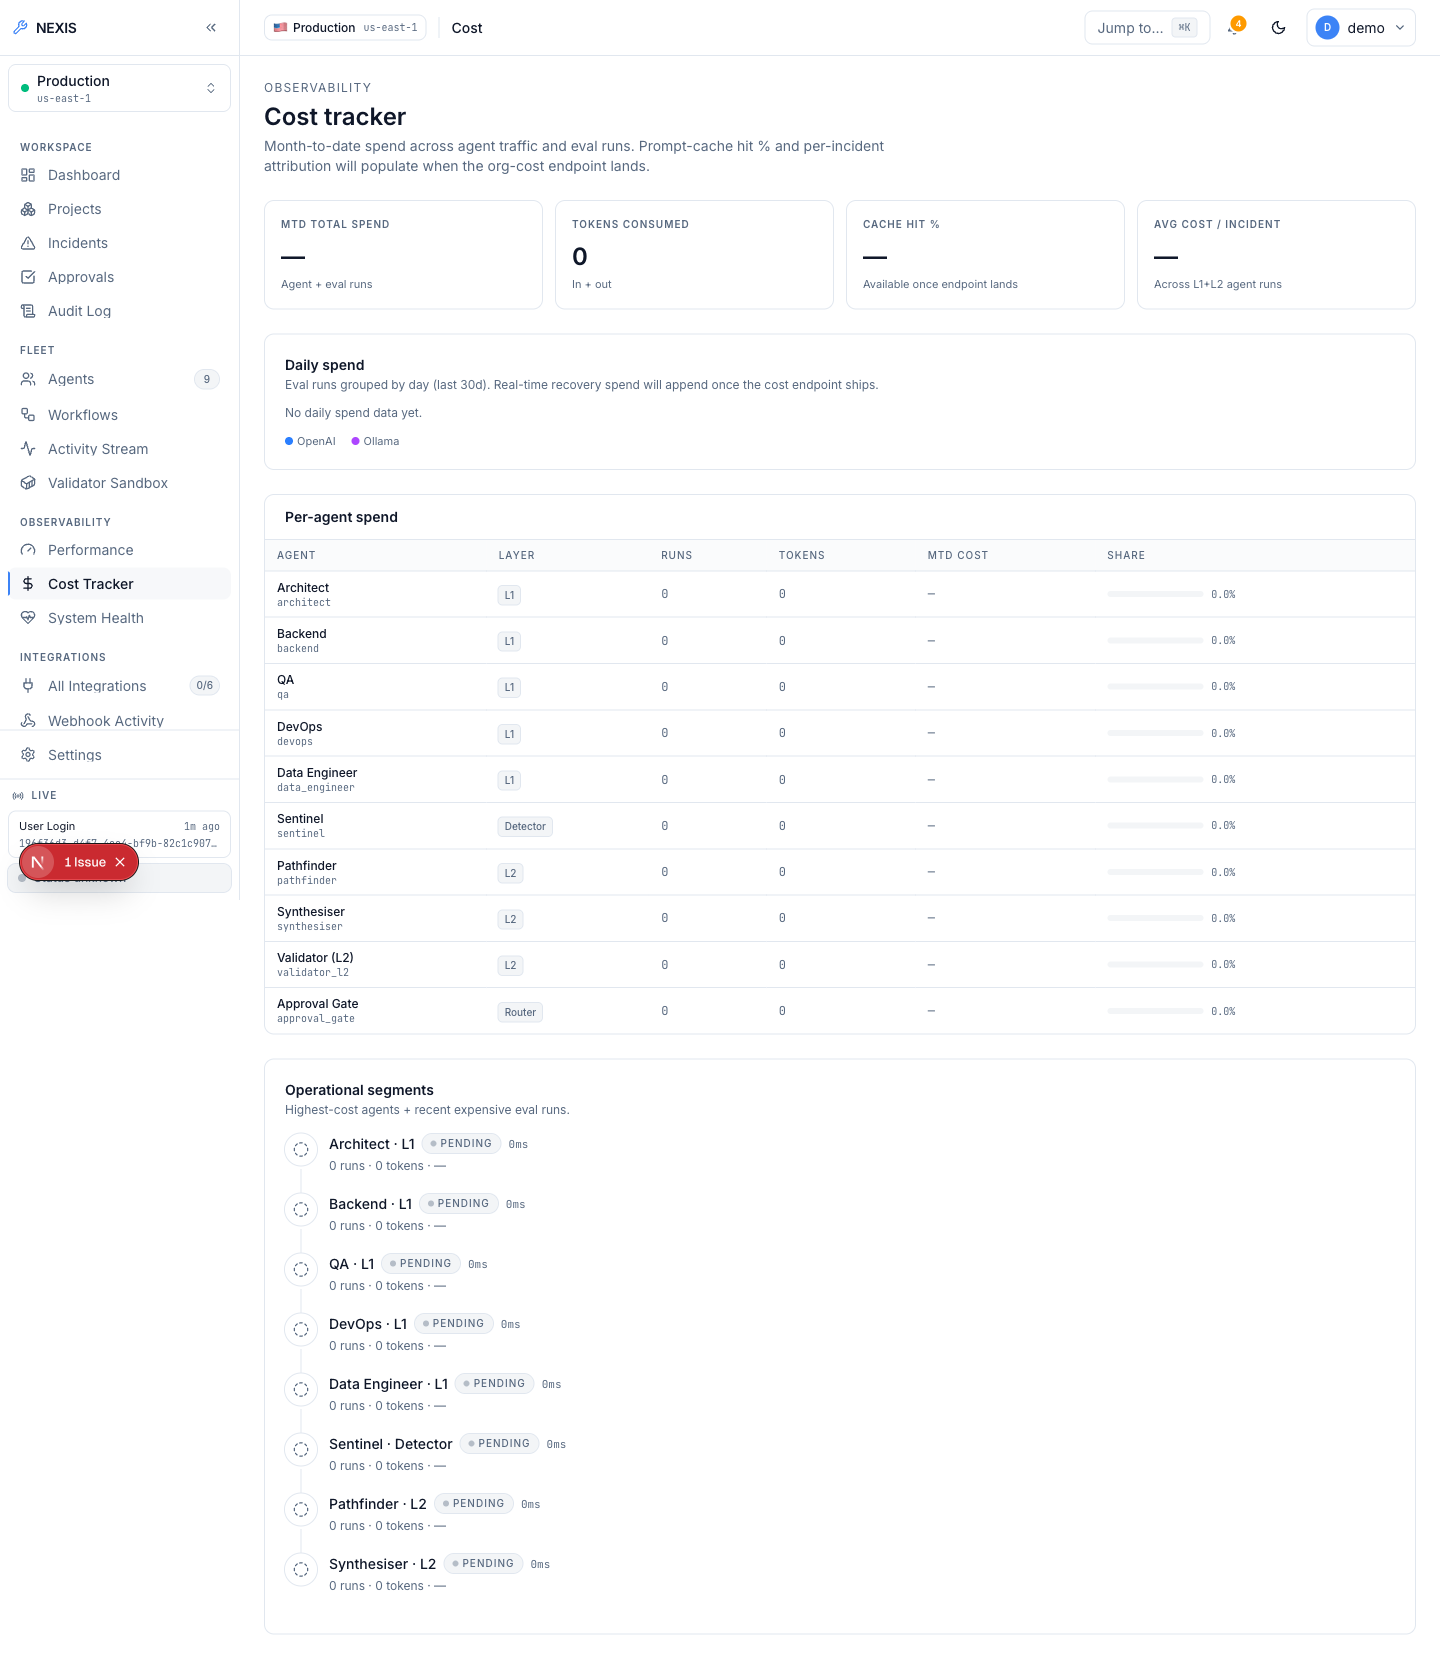
\includegraphics[width=0.85\textwidth]{../assets/screenshots/19-cost-tracker.png}
\caption{Cost Tracker ( per-organisation token ledger with daily budget ).}
\label{fig:cost}
\end{figure}

\begin{figure}[htbp]\centering
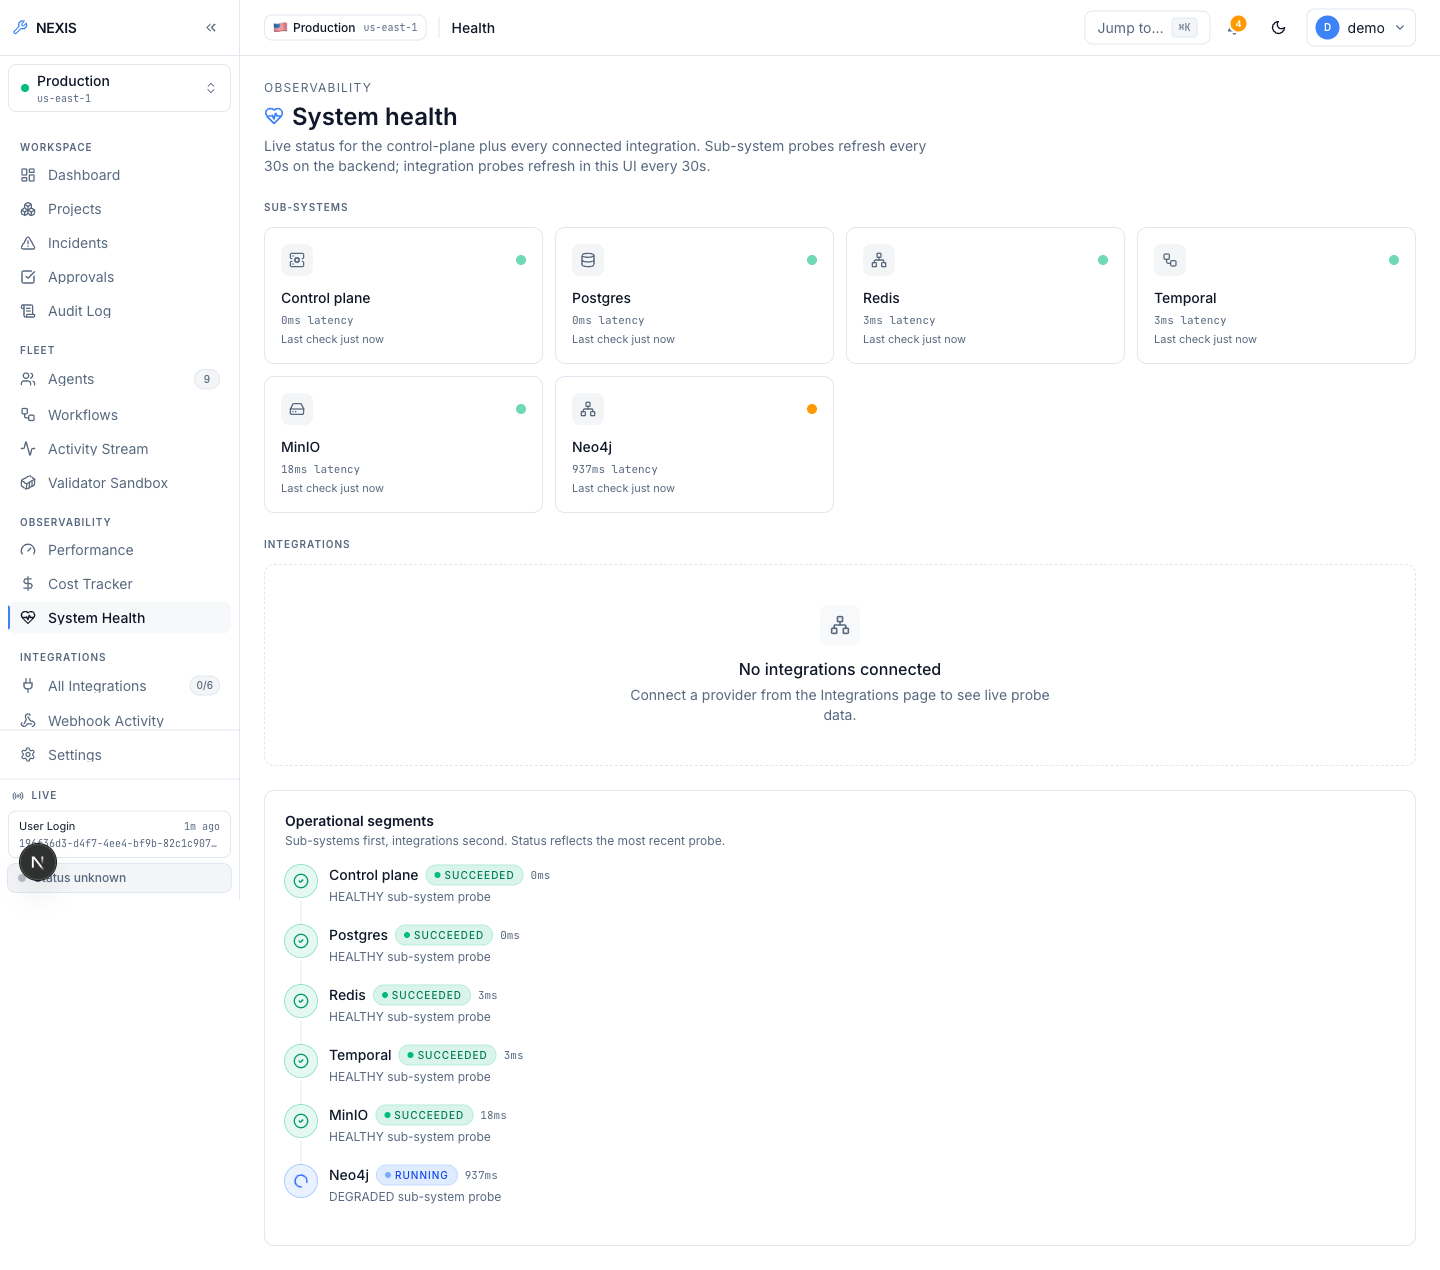
\includegraphics[width=0.85\textwidth]{../assets/screenshots/20-system-health.png}
\caption{System Health ( parallel dependency probes: Postgres, Redis, Neo4j, MinIO, Temporal ).}
\label{fig:health}
\end{figure}

\begin{figure}[htbp]\centering
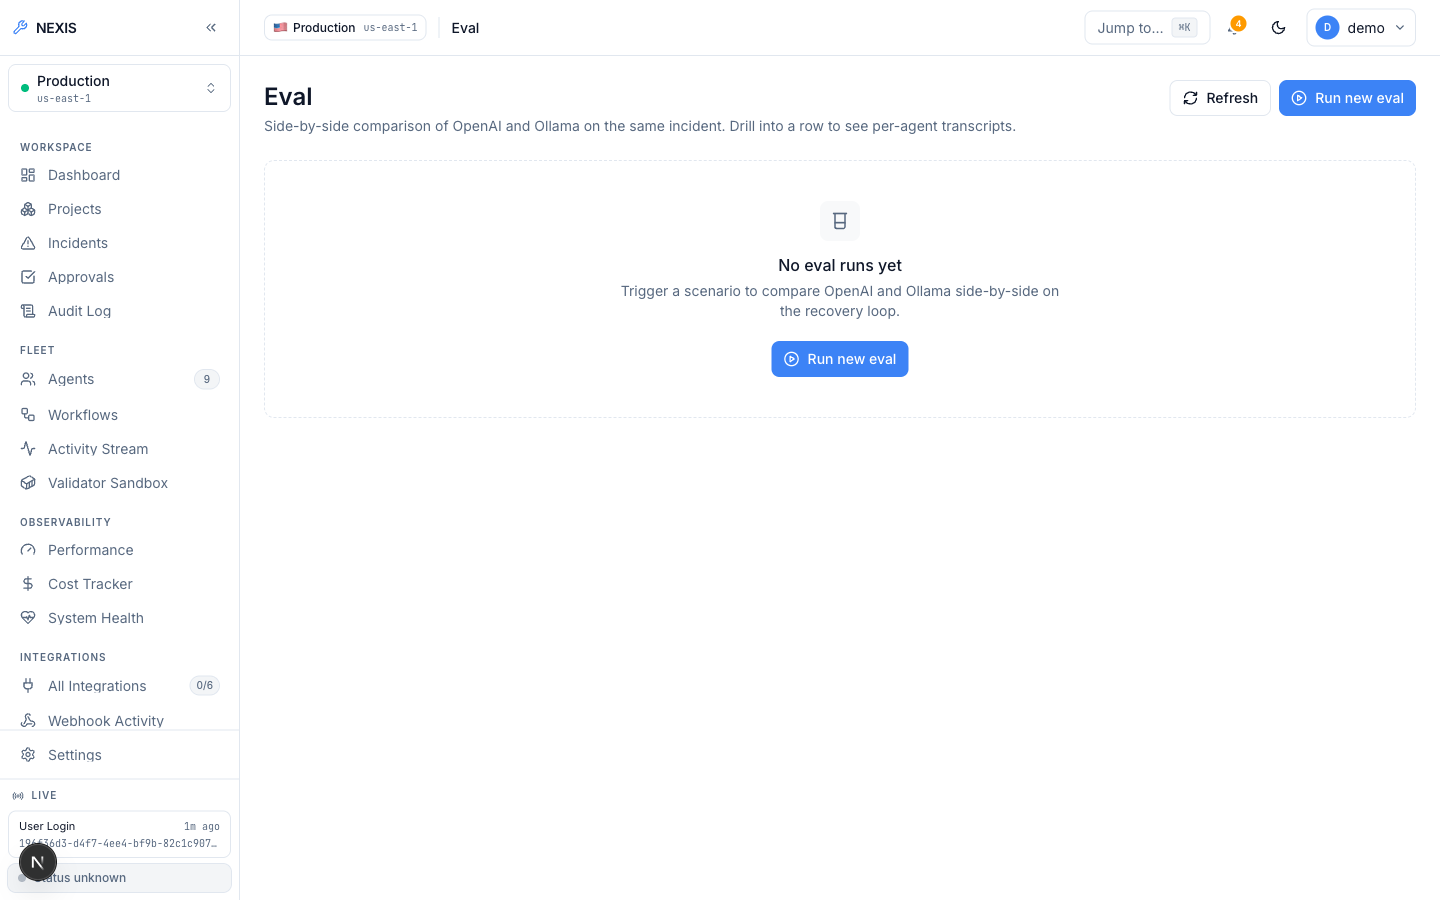
\includegraphics[width=0.85\textwidth]{../assets/screenshots/24-eval-harness.png}
\caption{Eval Harness ( side-by-side OpenAI-versus-Ollama comparison over fixture incidents ).}
\label{fig:eval}
\end{figure}

\begin{figure}[htbp]\centering
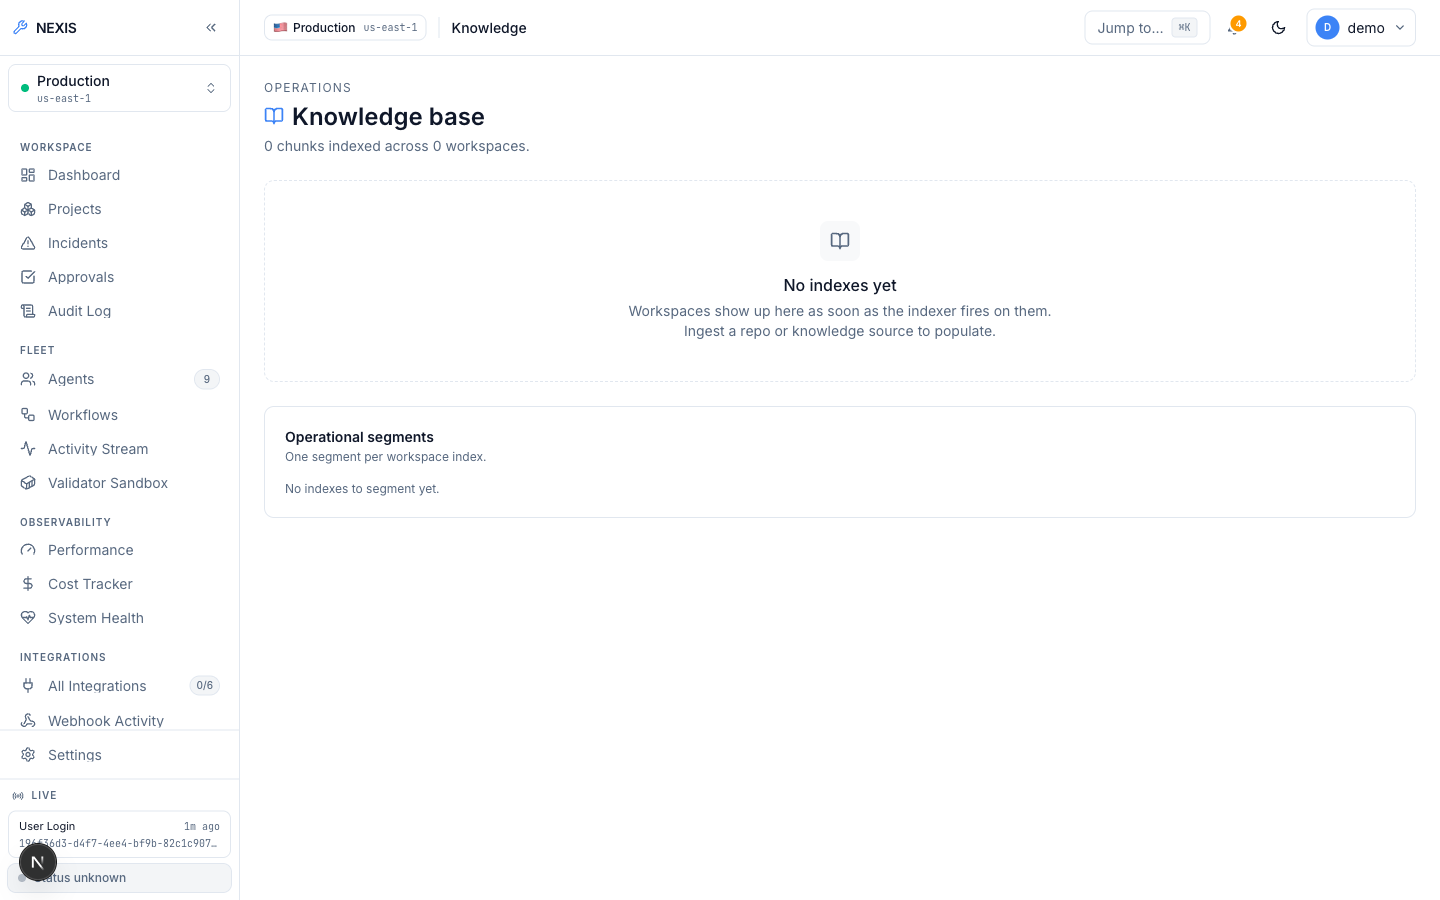
\includegraphics[width=0.85\textwidth]{../assets/screenshots/25-knowledge-base.png}
\caption{Knowledge Base ( pgvector-backed retrieval status ).}
\label{fig:kb}
\end{figure}

\subsection{Integrations}

The Integrations page (Figure~\ref{fig:integrations}) manages the external
providers the platform connects to: the GitHub App (installation, repository
listing, and webhook-driven incident creation on merged pull requests),
Sentry~\cite{sentry}, Datadog~\cite{datadog}, and PagerDuty~\cite{pagerduty}
as webhook-driven incident sources, Slack~\cite{slackapi} with OAuth install
and interactive one-click approve/reject directly from a Slack message,
Argo CD, and Stripe billing. Webhook Activity (Figure~\ref{fig:webhooks})
lists inbound webhook deliveries for debugging, and Connection Health
(Figure~\ref{fig:connhealth}) probes each configured integration and reports
its status.

\begin{figure}[htbp]\centering
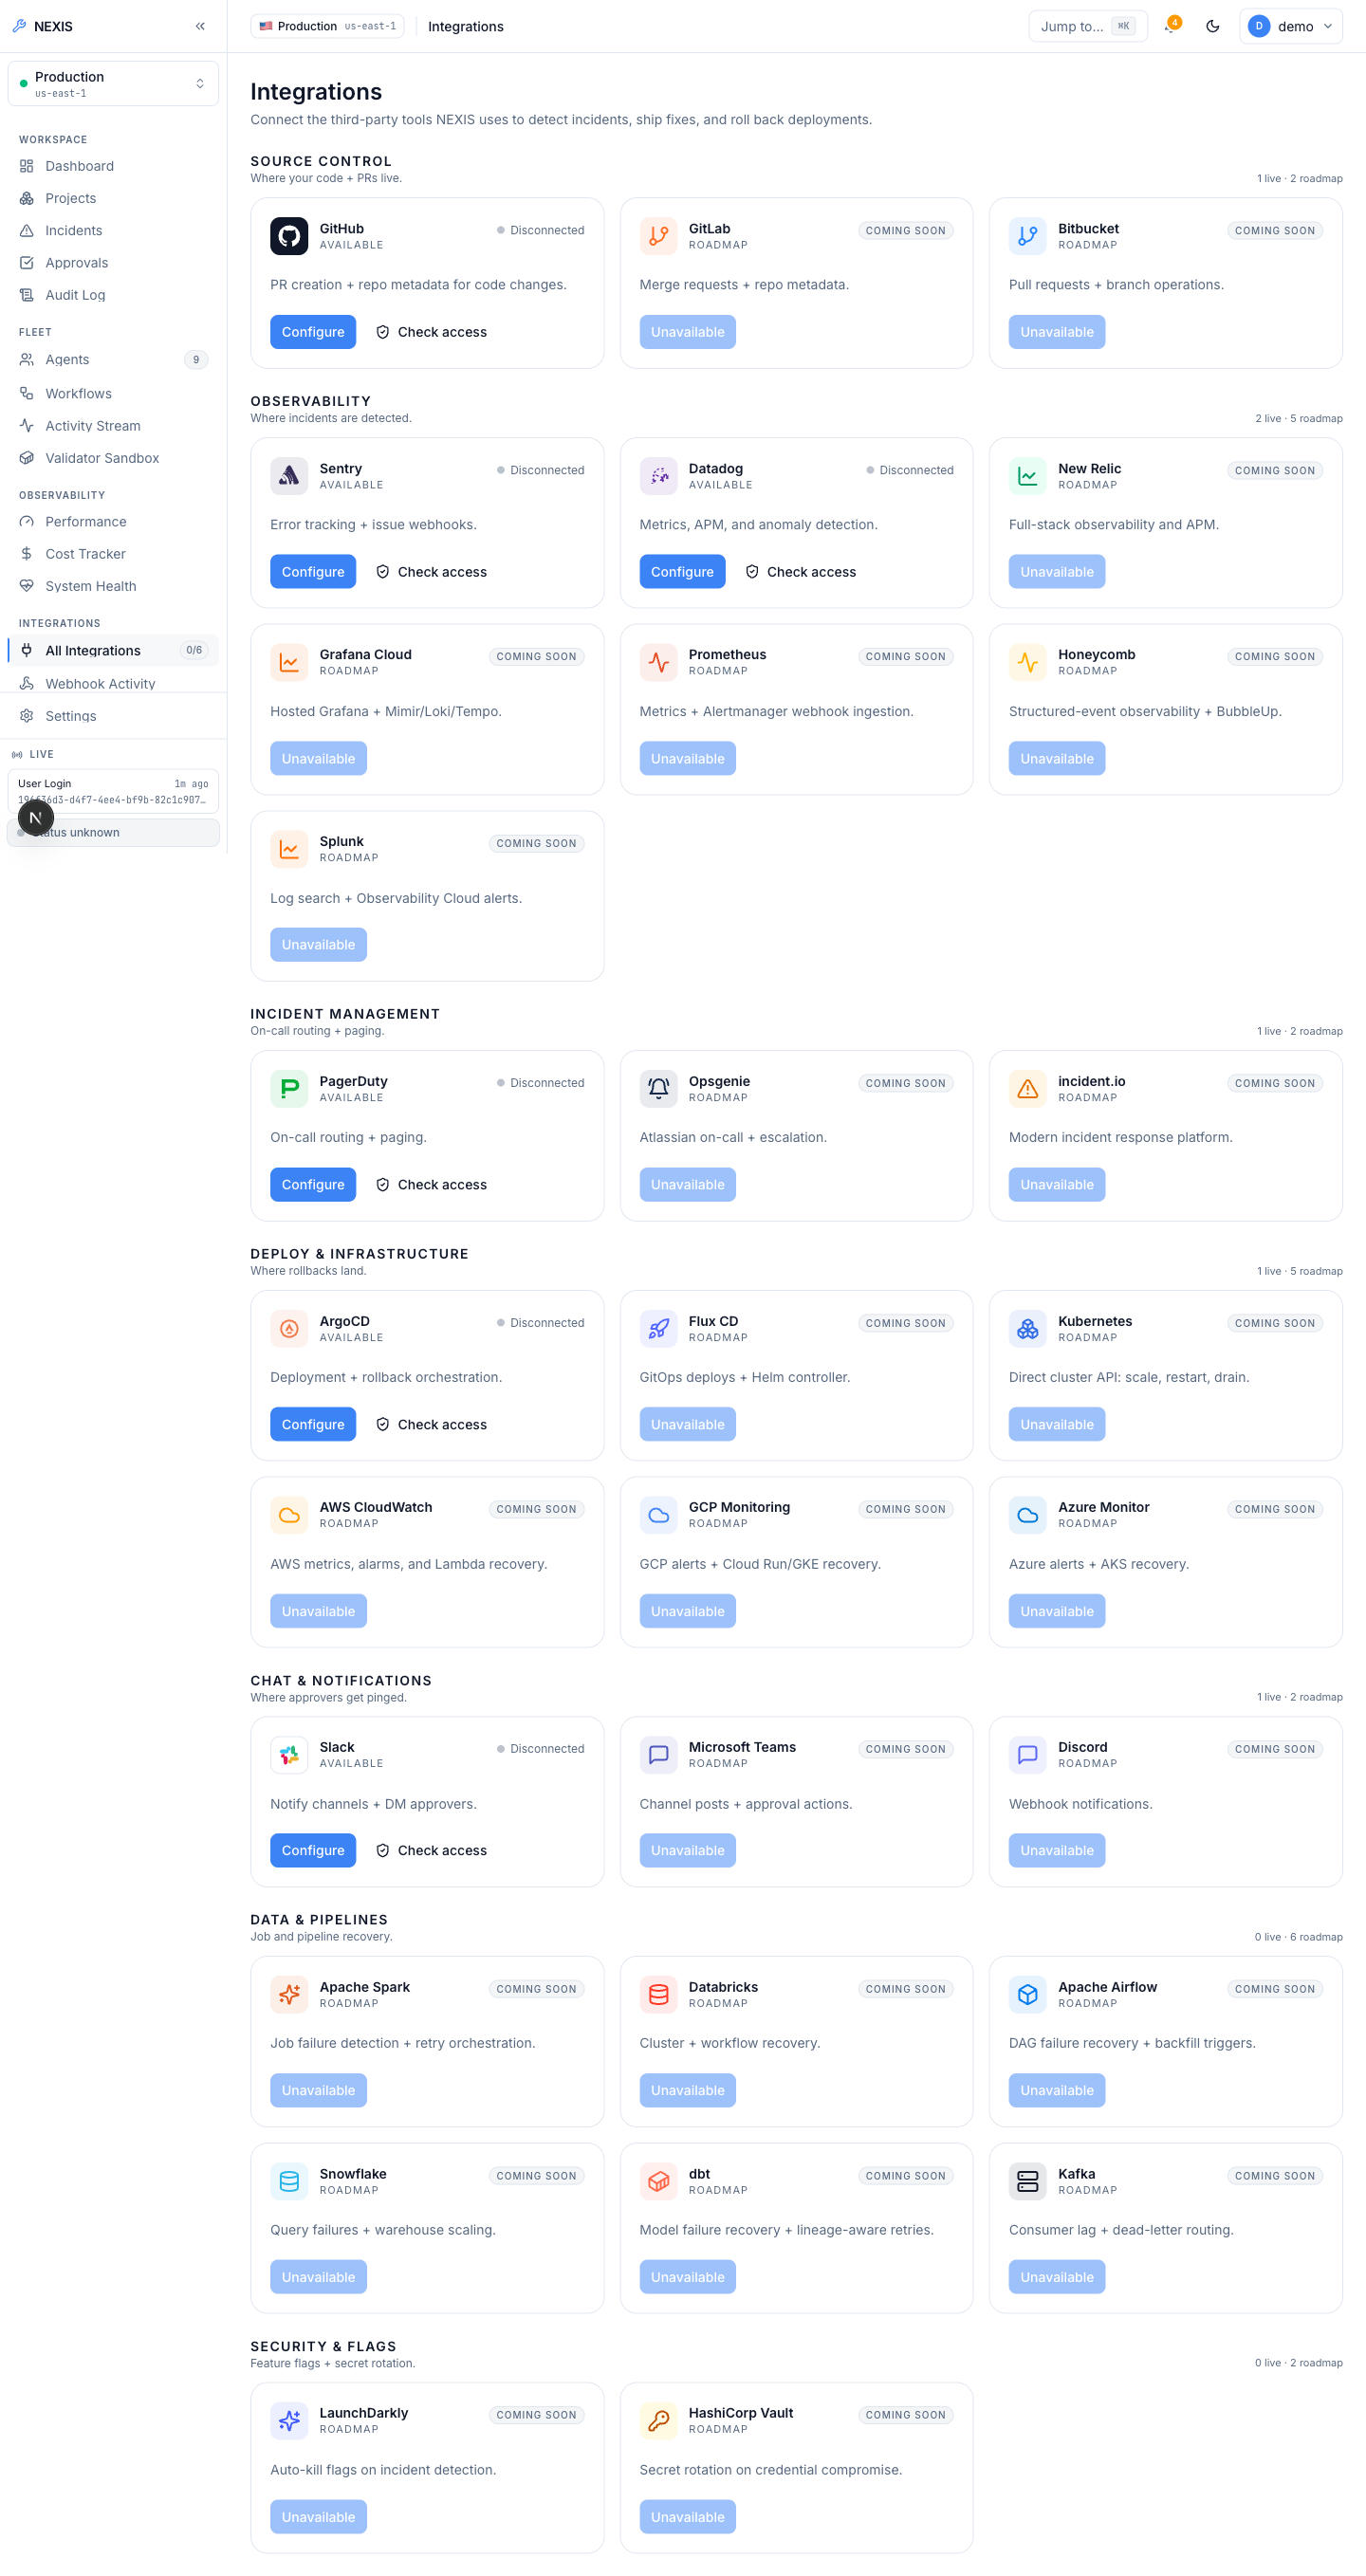
\includegraphics[width=0.85\textwidth]{../assets/screenshots/21-integrations.png}
\caption{Integrations Screen ( provider catalogue: GitHub App, Sentry, Datadog, PagerDuty, Slack, Argo CD, Stripe ).}
\label{fig:integrations}
\end{figure}

\begin{figure}[htbp]\centering
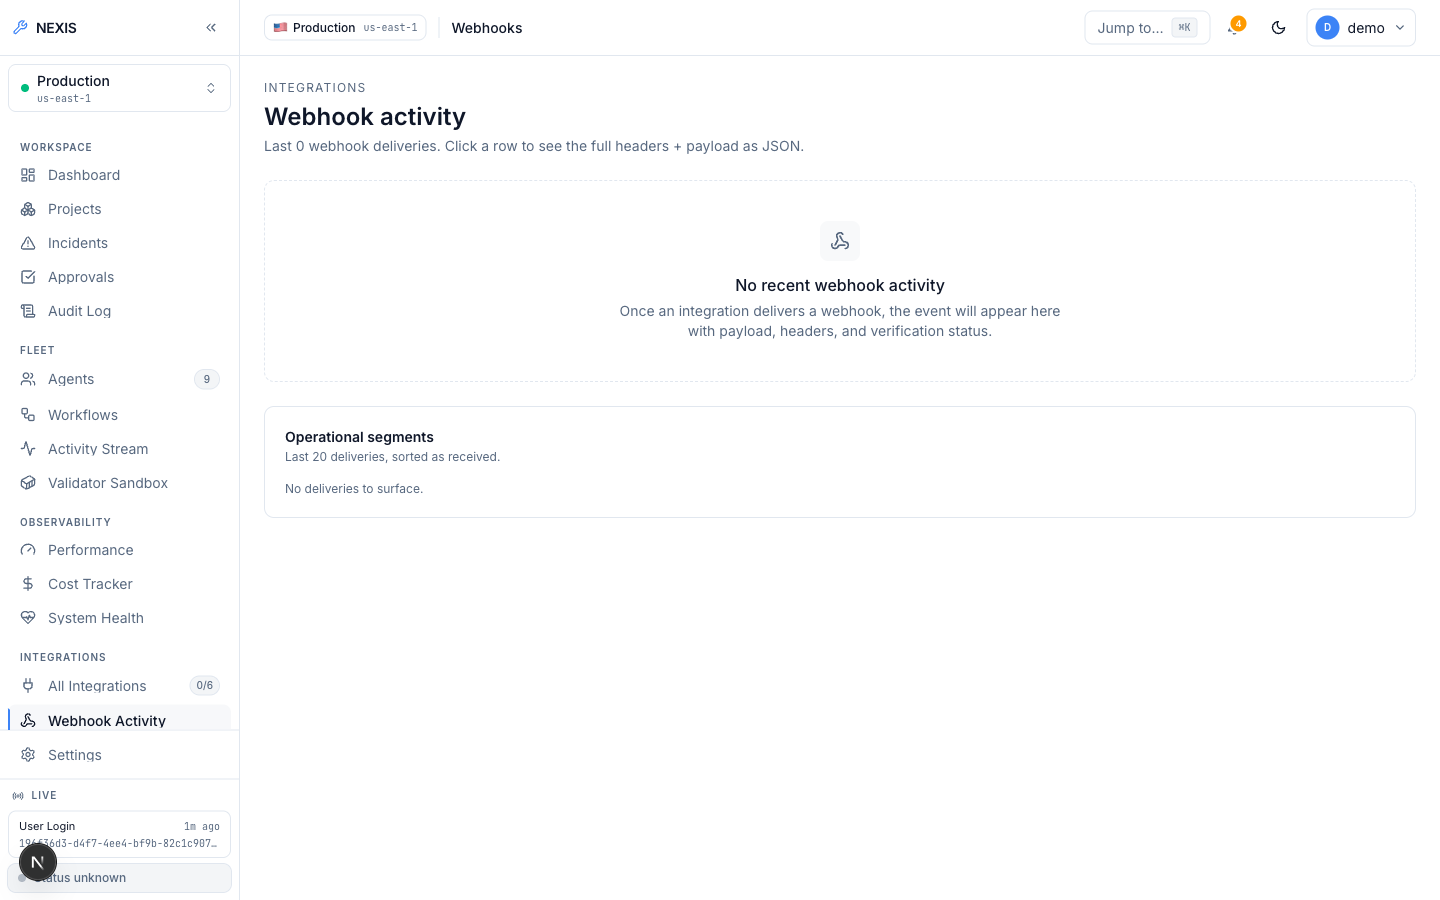
\includegraphics[width=0.85\textwidth]{../assets/screenshots/22-webhook-activity.png}
\caption{Webhook Activity ( inbound webhook delivery log ).}
\label{fig:webhooks}
\end{figure}

\begin{figure}[htbp]\centering
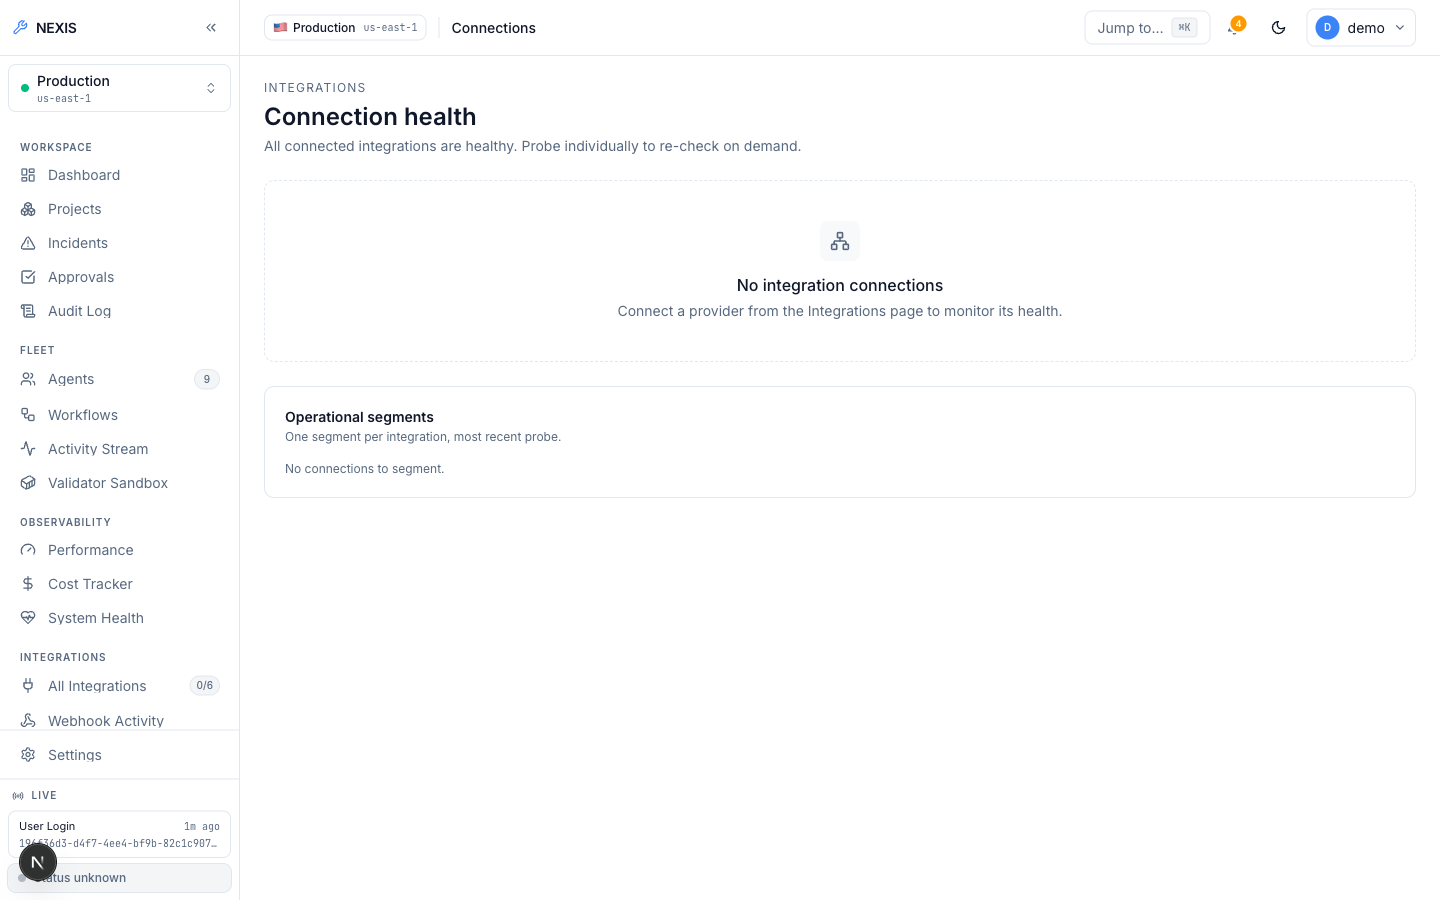
\includegraphics[width=0.85\textwidth]{../assets/screenshots/23-connection-health.png}
\caption{Connection Health ( per-integration health probes ).}
\label{fig:connhealth}
\end{figure}

\section{Database Schema}
\label{sec:schema}

Nexis stores its state in PostgreSQL~17. The schema has grown incrementally
across 33 sequential migrations, each tracked in version control alongside
the code that depends on it. Multi-tenancy is enforced in the database
itself rather than in application code: nearly every table carries an
organisation identifier, and PostgreSQL Row-Level Security
policies~\cite{pgrls} restrict every query to the calling organisation's
rows. A request-scoped transaction binds \code{app.current\_org\_id} for
each API request, so even a query that omits an explicit \code{WHERE}
clause on the organisation cannot read or write another tenant's data.

Table~\ref{tab:schema} summarises the key tables. Two deliberate exceptions
to org-scoping exist: \code{users} is a global identity table (a person may
belong to several organisations, with tenancy applied through
\code{org\_members}), and \code{sessions} is scoped to the owning user
rather than to an organisation, since a login session belongs to a person,
not a tenant.

\begin{table}[htbp]
\caption{Key tenant-scoped tables in the Nexis PostgreSQL schema.}
\label{tab:schema}
\centering
\small
\begin{tabular}{@{}p{3.6cm}p{7.2cm}p{2.9cm}@{}}
\toprule
\textbf{Table} & \textbf{Purpose} & \textbf{RLS scope} \\
\midrule
\code{users} & Global account identity: credentials, MFA enrolment, profile & Global (identity) \\
\code{org\_members} & User--organisation membership and role (owner / admin / member) & Org-scoped \\
\code{projects} & Registered projects, GitHub repository binding, recovery policy & Org-scoped \\
\code{incidents\_raw} & Every ingested fault event, from webhooks, fixtures, and the deploy engine & Org-scoped \\
\code{workflow\_runs} & One row per Temporal RecoveryPipeline execution, with per-step activity events & Org-scoped \\
\code{approval\_decisions} & Terminal approval-gate outcomes: approve, reject, modify, timeout & Org-scoped \\
\code{deployments} & Preview-deploy engine builds/containers and GitOps deployments & Org-scoped \\
\code{lineage\_events} & OpenLineage-compatible RunEvents~\cite{openlineage} for migration propose/apply & Org-scoped \\
\code{audit\_log} & Append-only, hash-chained record of privileged actions & Org-scoped \\
\code{feedback\_examples} & RLHF training rows persisted from every terminal approval decision & Org-scoped \\
\code{role\_recommendations} & Heuristic role-change recommendations with rationale and cool-down state & Org-scoped \\
\code{digest\_reports} & Daily admin digest aggregates (incidents, repairs, approvals, MTTR) & Org-scoped \\
\code{sessions} & Active login sessions: device, IP, user agent, last-seen & User-scoped \\
\code{api\_keys} & Scoped bearer keys (\code{nx\_live\_...}) for programmatic access & Org-scoped \\
\bottomrule
\end{tabular}
\end{table}

Beyond relational state, three specialised stores complete the data layer:
Neo4j holds the code dependency graph traversed by the Pathfinder agent,
MinIO holds encrypted patch blobs referenced from \code{workflow\_runs}, and
pgvector columns inside PostgreSQL back the knowledge-base retrieval
feature. Temporal maintains its own durable persistence for workflow event
histories, which complements --- and in a recovery scenario can reconstruct
--- the per-step records in \code{workflow\_runs}.
